% This template was originally by R. Jacob Vogelstein
% Updated on March 1, 2010 by Noah J. Cowan
% Finally put to use by Andrew Whitbeck 2013

\documentclass[12pt,oneside,final]{thesis}

\usepackage{mathtools}
\usepackage{setspace}
\usepackage{feynmp}
\usepackage{rotating}
\usepackage{cite}
\usepackage{amsmath,amsfonts}
\usepackage{amssymb}
\usepackage{graphicx}
\usepackage{mathrsfs}
\usepackage{color}
\graphicspath{{./figs/}}
\usepackage{fixltx2e}
\usepackage{array}
% wrapfig is fragile: use sparingly
\usepackage{wrapfig} 
%\usepackage{times}  % Use this for ugly fonts


\usepackage{fancyhdr}    % Use nice looking headers along with the required footer page numbers   
%\usepackage[hypertex]{hyperref}

%Define the header/footer style
\pagestyle{fancy}
\fancyhf{}
\setlength{\headheight}{15pt}
\lhead{\leftmark}
\cfoot{\thepage}
\renewcommand{\headrulewidth}{0pt}
\fancypagestyle{plain}{% Redefine ``plain'' style for chapter boundaries
\fancyhf{} % clear all header and footer fields
\fancyfoot[C]{\thepage} % except the center
\renewcommand{\headrulewidth}{0pt}
\renewcommand{\footrulewidth}{0pt}}

%\tolerance=10000

%\makeglossary % enable the glossary

\begin{document}

\title{DISCOVERY AND CHARACTERIZATION OF A HIGGS-LIKE RESONANCE
USING THE MATRIX ELEMENT LIKELIHOOD APPROACH}
\author{Andrew J. Whitbeck}
\degreemonth{September}
\degreeyear{2013} 
\dissertation
\doctorphilosophy
\copyrightnotice

% add your chaptders, best way is to have separate TeX files for each chapter
%% FRONTMATTER
\begin{frontmatter}

% generate title
\maketitle

\begin{abstract}
Understanding the exact mechanism of electroweak symmetry breaking
through the discovery and characterization of the Higgs boson
is one of the primary goals of the Large Hadron Collider (LHC).
Two searches for a Higgs boson decaying to a pair of Z bosons
with subsequent decays to either $2\ell2q$ or $4\ell$ are 
presented using data
recorded with the Compact Muon Solenoid (CMS). 
The discovery and characterization of a Higgs-like resonance
using a new set of tools is reported.  
The foundations of 
such tools are developed and prospects for their use
in other Higgs channels and at future colliders are addressed.
Although the Standard
Model (SM) of electroweak interactions has been extremely
successful in describing a number of phenomena, there are still
questions to be addressed pertaining to its naturalness and its
possible connection to beyond the SM physics.  
Results are interpreted in the context of possible
extensions to the SM and their effect on our understanding of
the universe.
\vspace{.3cm}
\noindent Primary Reader: Andrei Gritsan\\
Secondary Reader:

\end{abstract}

\begin{acknowledgment}

I would like to thank Andrei Gritsan for accepting me as a student.
I am lucky to have been a part of developing the great ideas that
have resulted from his research program and have learned an 
immense amount physics and how to approach research problems.  
I have been fortunate to take on a leading role in
my field and to represent my collaboration on more than one 
occasion as an ambassador to the greater scientific community. 
This would not have been possible with his encouragement and
guidance.

I would also like to thank everyone involved with CMS and the
LHC.  It has been a remarkable experience to be 
a part of the collaboration and see what can be done when
thousands of people put their minds to one big idea.  
I would also like to give special thanks to all the 
CMS research groups: te Higgs PAG, HZZ subgroup, and tracker 
alignment group.  
I am eternally grateful for those who have supported me
in my continue academic career: Chiara, Joe, Andrey, and Yves. 

\end{acknowledgment}

%\begin{dedication} 

%\end{dedication}

% generate table of contents
\tableofcontents

% generate list of tables
\listoftables

% generate list of figures
\listoffigures

\end{frontmatter}

\chapter{Introduction}
\label{sec:intro}
\chaptermark{Theoretical Motivation}
Modern particle physics is described by a theory called the standard model (SM).  
The SM describes a universe in which matter consists of particles of half-integer spin\footnote{Intrinsic angular momentum} called fermions.  
These fermions interact with each other through force mediating integer spin particles called bosons.  
This section will provide a basic outline of this theory as well as the known issues and need for a more basic theory.

\section{Fundamental Particles}
The SM matter in the universe is around 98\% Hydrogen and Helium with the final 2\% being heavier elements.  
To a very good approximation, the known matter in the universe consists of protons, neutrons, and electrons.  
Electrons are categorized in the standard model as leptons and are fundamental.  
Protons and neutrons are composites of three quarks.  
The up quark (u) has +2/3e\footnote{e is the magnitude of the charge of the electron} charge, and the down quark (d) has -1/3e charge, so the proton is an up-up-down combination and the neutron is down-down-up.  
These quark compounds are called hadrons and are categorized into two families: baryons (three quarks), and mesons (two quarks).

Although this is a good approximation of the known universe, through experimental and theoretical advances we know that there are 
more exotic phenomena that can be described by extending the known quarks and leptons to three generations.  
The three lepton generations are defined by the electron, muon, tau and their corresponding neutrinos.
The +2/3e charge quarks are the up, charm, and top; whereas the -1/3e charge quarks are the down, strange, and bottom.  
These quarks and leptons are summarized in Table~\ref{table:SMferm} along with their charge and mass.
    
Quarks and leptons define all known fermionic matter, with bosonic particles being responsible for particle interactions.
    

\begin{table}[h]
\begin{center}
\begin{tabular}{l|c|c}
\hline
\hline
particle & charge (e) & mass (MeV)\\ \hline \hline
e & -1 & 0.5110 \\
$\mu$ & -1 & 105.7\\
$\tau$ & -1 & 1777\\
$\nu_{\mathrm{e}}$, $\nu_{\mu}$, $\nu_{\tau}$ & 0 & $<$ 2 $\times \mathrm{10^{-6}}$ \\
u & +2/3 & 2.3\\
d & -1/3 & 4.8\\
s & -1/3 & 95\\
c & +2/3 & 1.275 $\times \mathrm{10^3}$ \\
b & -1/3 & 4.18 $\times \mathrm{10^3}$\\
t & +2/3 & 173.2 $\times \mathrm{10^3}$\\
\hline
\end{tabular}
\end{center}
\caption{List of SM fermions with their charge and mass.  These particles all have spin 1/2.}
\label{table:SMferm}
\end{table}


\section{Fundamental Interactions}
Interactions in the SM can be described by the four fundamental forces: electromagnetic, weak nuclear, strong nuclear, and gravity.  
These forces manifest by the exchange of a corresponding elementary boson.  
The intrinsic properties of these force carrying particles are responsible for the range and relative strength of the interaction.


The electromagnetic force is responsible for well known phenomena such as molecular bonds.  
This force is mediated be the photon, a massless, charge-less, spin 1 particle.  
The photon interacts with charged particles only.        
The fact that the photon is massless leads to the infinite range of the electromagnetic force.  


The weak nuclear force manifests itself in nuclear decay, and is described by three force carrying bosons; the $\mathrm{W^+}$,$\mathrm{W^-}$, and Z.  
These bosons are massive, which leads to the weak force being short range.  
The $W^{\pm}$ bosons have integer charge whereas the Z boson is charge-less, and all three have spin 1.  
The weak force is responsible for transitions between flavors\footnote{The six quark types} of quarks (see Section~\ref{sec:weaktheory}).
Quarks and leptons alike interact by the weak force.


The strong nuclear force is responsible for binding quarks together to form hadrons.  
The strong force describes the interactions of particles that carry color.  
Color is an intrinsic property of fundamental particles, and has three varieties; red, green and blue.
This force is mediated by gluons, which are massless and interact with quarks.  
The strong force is the strongest and shortest range of the known forces.  
The theory behind the strong force is described in more detail in Section~\ref{sec:qcdtheory}

The known force carrying bosons and their properties are listed in table \ref{table:SMbos}

The fourth known force, gravity, is both the most recognizable and least understood of the forces.  
All attempts at including gravity into the SM have failed, but hypothetically gravity should be mediated by the spin 2 graviton, which interacts with massive particles..
Gravity is by far the weakest of the fundamental forces. 


\begin{table}
\begin{center}
\begin{tabular}{l|c|c|c}
\hline
\hline
particle & charge (e) & spin & mass (GeV)\\ \hline \hline
$\gamma$  & 0 & 1 & 0\\ 
$\mathrm{W^{\pm}}$ & $\pm$1 & 1 & 80.4\\
Z & 0 & 1 & 91.2\\ 
gl & 0 & 1 & 0 \\ 
gr & 0 & 2 & $<$ 6 $\times$ $\mathrm{10^{-38}}$ \\ 
\hline
\end{tabular}
\end{center}
\caption{List of SM force carrying bosons with their charge, mass and spin.  The graviton has not yet been observed.}
\label{table:SMbos}
\end{table}


\section{Feynman Diagrams}
Calculations in theoretical particle physics are facilitated by the use of feynman diagrams.  
Feynman diagrams are pictorial representations.  
These diagrams include the particles that interact (external lines), as well as the particles that mediate the interaction (internal lines), 
and where these external and internal lines intersect (vertices).
An example diagram is shown in Figure~\ref{figs:emuScattering}.  
The electrons interact with a photon ($\gamma$), and a force is observed.
This diagram represents electromagnetic repulsion (coulomb force).  

\begin{figure}
\begin{center}
\unitlength=1mm
\begin{fmffile}{feynman/emuScattering}
\begin{fmfgraph*}(40,30) \fmfpen{thick}
\fmfleft{i1,i2} \fmfright{sp1,sp2}
\fmf{fermion}{i1,v1,sp1}
\fmf{fermion}{sp2,v2,i2}
\fmf{photon,label=$\gamma$}{v1,v2}
\fmflabel{$e^-$}{i1}
\fmflabel{$e^+$}{i2}
\fmflabel{$e^-$}{sp1}
\fmflabel{$e^+$}{sp2}
\end{fmfgraph*}
\end{fmffile}
\end{center}
\caption{Feynman diagram depicting electron-positron scattering via
the electromagnetic interaction.}
\label{figs:emuScattering}
\end{figure}


The rules governing the calculation of physical observables from these diagrams are defined by the theory of Quantum Electrodynamics (QED).
Using these diagrams, the rules of QED let us calculate the matrix element ($\cal{M}$).  
$\cal{M}$ can by related to physical quantities through the square modulus ($|\cal{M}|^{\mathrm{2}}$), which is the probability density for a process to occur.   
From this, relevant quantities such as the cross section (see Section~\ref{sec:LumiXsec}) of the process can be calculated.  

Additionally, in the case that a particle decays we can evaluate the decay width ($\Gamma$).  
When a particle of mass M decays, there is a range of observed values of mass following a Breit-Wigner distribution centered at M.
The decay width represents the width of this distribution at half the maximum.  The average lifetime of the particle is 1/$\Gamma$.

For a given process there can be multiple contributing diagrams, for instance for a calculation involving the Coulomb attraction shown in Figure~\ref{figs:emuScattering}, 
one must also consider the 
diagrams shown in Figure~\ref{figs:emuScattering2}, which have the same incoming and outgoing particles.  
Diagrams such as this interfere with each other constructively or destructively in the calculation of the matrix element, 
which can increase or decrease the cross section of the full process.

\begin{figure}
\begin{center}
\unitlength=1mm
\begin{fmffile}{feynman/emuScattering1}
\begin{fmfgraph*}(40,30) \fmfpen{thick}
\fmfleft{i1,i2} 
\fmfright{sp1,sp2}
\fmf{fermion}{v1,i1}
\fmf{phantom}{v1,sp1}
\fmf{fermion,tension=0}{v2,sp1}

\fmf{phantom}{v2,sp2}
\fmf{fermion,tension=0}{sp2,v1}

\fmf{photon,label=$\gamma$}{v1,v2}

\fmf{fermion}{i2,v2}

\fmflabel{$e^-$}{i1}
\fmflabel{$e^+$}{i2}
\fmflabel{$e^+$}{sp1}
\fmflabel{$e^-$}{sp2}

\end{fmfgraph*}
\end{fmffile}
\end{center}
%\caption{Feynman diagram depicting electron-positron scattering via
%the electromagnetic interaction in the u channel.}
%\label{figs:emuScattering1}
\end{figure}


\begin{figure}
\begin{center}
\unitlength=1mm
\begin{fmffile}{feynman/emuScattering2}
\begin{fmfgraph*}(40,30) \fmfpen{thick}
\fmfleft{i1,i2} \fmfright{sp1,sp2}
\fmf{fermion}{i1,v1,i2}
\fmf{fermion}{sp2,v2,sp1}
\fmf{photon,label=$\gamma$}{v1,v2}

\fmflabel{$e^-$}{i1}
\fmflabel{$e^-$}{i2}
\fmflabel{$e^-$}{sp1}
\fmflabel{$e^-$}{sp2}


\end{fmfgraph*}
\end{fmffile}

\end{center}
\caption{Feynman diagram depicting electron-positron scattering via
the electromagnetic interaction in the u channel (top) and s channel (bottom).}
\label{figs:emuScattering2}
\end{figure}


Vertices in a Feynman diagram are points where energy and momentum are conserved in the calculation.  
Each of the vertices contributes a factor of the coupling constant $\alpha$ to the matrix element computation.  
In the calculation of the full matrix element for the electron positron attraction shown in Figures~\ref{figs:emuScattering} and~\ref{figs:emuScattering2}, 
we must consider diagrams with higher vertex multiplicity such as those seen in Figure~\ref{figs:emuScatteringnlo2}.  
To approximate $\cal{M}$ in QED, we can perform an expansion in the vertex multiplicity n, summing over matrix elements within the same order i ($\cal{M}_{\mathrm{i}}^{\mathrm{n}}$). 
 .  

\begin{figure}
\begin{center}
\unitlength=1mm
\begin{fmffile}{feynman/emuScatteringnlo1}
\begin{fmfgraph*}(40,30) \fmfpen{thick}
\fmfleft{i1,i2} \fmfright{sp1,sp2}
\fmf{fermion,tension=1.5}{i1,m1,v1,m2,i2}
\fmf{fermion}{sp2,v2,sp1}
\fmf{photon,label=$\gamma$}{v1,v2}
\fmf{photon,tension=0.0,left}{m1,m2}
\fmflabel{$e^-$}{i1}
\fmflabel{$e^-$}{i2}
\fmflabel{$e^-$}{sp1}
\fmflabel{$e^-$}{sp2}
\end{fmfgraph*}
\end{fmffile}
\end{center}
%\caption{Feynman diagram depicting NLO electron-positron scattering via
%the electromagnetic interaction.}
%\label{figs:emuScatteringnlo1}
\end{figure}

\begin{figure}
\begin{center}
\unitlength=1mm
\begin{fmffile}{feynman/emuScatteringnlo2}
\begin{fmfgraph*}(40,30) \fmfpen{thick}
\fmfleft{i1,i2} \fmfright{sp1,sp2}
\fmf{fermion}{i1,v1,i2}
\fmf{fermion}{sp2,v4,sp1}
\fmf{photon}{v1,v2}
\fmf{fermion,tension=0.5,left}{v2,v3,v2}
\fmf{photon}{v3,v4}
\fmflabel{$e^-$}{i1}
\fmflabel{$e^-$}{i2}
\fmflabel{$e^-$}{sp1}
\fmflabel{$e^-$}{sp2}
\end{fmfgraph*}
\end{fmffile}
\end{center}
\caption{Feynman diagram depicting NLO electron-positron scattering.}
\label{figs:emuScatteringnlo2}
\end{figure}


\begin{eqnarray}
\cal{M} = \sum\limits_{\mathrm{n=1}}^\infty \sum\limits_{\mathrm{i}}  \cal{M}_{\mathrm{i}}^{\mathrm{n}}
\label{eqn:matrixelement}
\end{eqnarray}  

Due to the fact that the coupling constant in QED is 1/137, this expansion can terminate quickly because high n diagrams contribute much less to $\cal{M}$.  
A calculation involving all diagrams with the least number of vertices is called leading order.  
Calculations involving all diagrams with higher order contributions as well are called next-to leading order (NLO), next-to-next-to leading order (NNLO), etc.    

Once the matrix element has been determined to an acceptable accuracy, we can extract the cross section in a straight forward manner.  
For the example electron-positron scattering process above the differential cross section has the following simplified equation due to the special case of identical mass particles:  

\begin{eqnarray}
\left(\frac{\mathrm{d\sigma}}{\mathrm{d\Omega}}\right)_{\mathrm{CM}} = \mathrm{\frac{|\cal{M}|^{\mathrm{2}}}{64 \pi^{2} E_{cm}^{2}}}
\label{eqn:xsecfromsigma}
\end{eqnarray}  


\section{Quantum Chromodynamics}
\label{sec:qcdtheory}
Quantum chromodynamics (QCD) is the theory describing the strong force, and is of particular importance for this thesis.  
The strong force is mediated by gluons which interact with particles that carry color.  
In QED, the photon is not charged, and thus can not interact with itself, however in QCD the gluon carries color and thus can interact with itself.  
Additionally, whereas the addition of a vertex greatly reduces the cross section in QED, the strong coupling constant $\alpha_s$ is of order 1, so 
higher order diagrams can contribute substantially to the measurement.  This means that QCD processes are much more difficult to calculate than QED 
processes.

However, $\alpha_s$ is not constant, and in fact increases as the distance scale of an interaction increases (see Figure~\ref{figs:alphasrunning}).  
This property of the the strong interaction is called asymptotic freedom.  For high $|q^2|$, $\alpha_s$ has the following form:

\begin{eqnarray}
\mathrm{\alpha_{s}(|q^2|)} =  \frac{\mathrm{\alpha_{s}(\mu^{2})}}{\mathrm{1+(\alpha_{s}(\mu^{2})/12\pi)(11n-2f)ln(|q^2|/\mu^{2})}}
\label{eqn:qcdalphas}
\end{eqnarray}  
%from Griffiths

where n is the number of colors (3), and f is the number of flavors (6), and $\mu^{2}$ is some arbitrary energy where $\alpha_{s}(\mu^{2})$ $<$ 1.
Therefore because 11n $>$ 2f, $\alpha_{s}$ will decrease as energy increases.


Therefore as the distance between two quarks increases, so do the forces holding them together.  
This large force at a characteristic distance ($\sim10^{-15}$ m) is the reason why it is difficult to observe a free quark (quark confinement).  
Although quarks can not be observed alone, there are ways of precisely determining the physical properties of free quarks through reconstruction of their decay products.  




\begin{figure}
\begin{center}
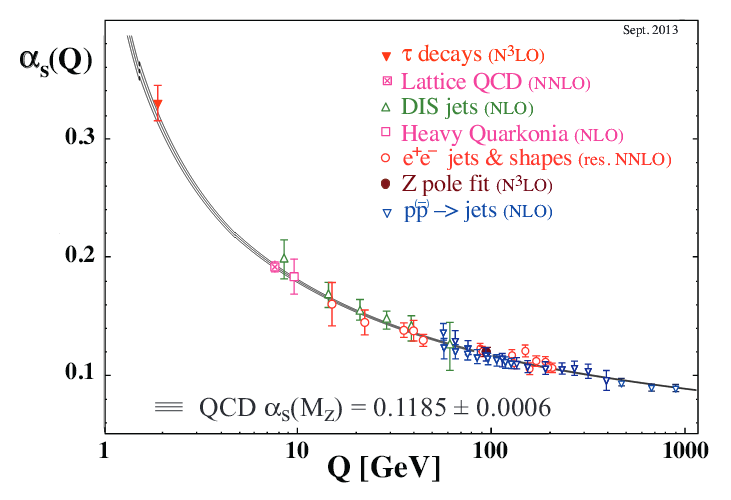
\includegraphics[width=1.0\linewidth]{figs/alphasrunning.png}
\caption{The QCD coupling constant $\alpha_{\mathrm{S}}$ as a function of the energy scale Q.}
\label{figs:alphasrunning}
\end{center}
\end{figure}
%from pdg


When a quark pair is produced with a high momentum, their separation increases quickly.  
As the separation of these quarks increases, the energy of the QCD field between them increases as well.  
If this separation is high enough, the energy between the quarks will reach a threshold where quark pair production is energetically favorable.  
At this threshold, the constituent quarks are then joined by these pair produced quarks.  
Additional quark pairs can be created many times, and the initial quark is detected as many hadrons that are collimated into a stream of particles called a jet.  
This process is called hadronization, 

The $\alpha_s$ parameter is low at short distances (or equivalently high energy); 
just like in QED, the impact of higher order diagrams is low.  
This allows the calculation of QCD diagrams using a finite perturbative expansion, and allows us to only consider only free quarks in high energy QCD calculations. 
The characteristic interaction energy where free quarks can be considered is around 400$\MeV$, which is much lower than energy scales 
considered in this thesis, so we will only be referring to free quark interactions.  


\section{The Weak Force}
\label{sec:weaktheory}
The weak force is felt by quarks and leptons alike.  
It is weaker than both the electromagnetic and the strong force, which leads to longer decay times for weakly decaying particles.  
The weak force is responsible for changing of quark flavor in an interaction.  
A vertex involving a change is quark flavor contributes a factor of $V_{ij}$ to the matrix element, where $V_{ij}$ is an element of the Cabibbo Kobayashi Maskawa (CKM) matrix 
(shown in Figure\ref{figs:CKM}).  
For example, the calculation of the diagram in Figure~\ref{figs:betaDecay} (beta decay) includes a factor of $V_{ud}$ = 0.97427.  
The CKM matrix is roughly diagonal, which means that a process which changes quark generation is rare.  

\begin{figure}
\begin{center}
\unitlength=1mm
\begin{fmffile}{feynman/betaDecay}
\begin{fmfgraph*}(40,30) \fmfpen{thick}
\fmfleft{i1,i2} \fmfright{sp1,sp2,sp3}
\fmf{phantom}{i2,v2,sp3}
\fmf{fermion}{i1,v1,sp1}
\fmf{fermion,tension=0.0}{v2,sp2}
\fmf{fermion,tension=0.0}{sp3,v2}
\fmf{photon,label=$W^{-}$}{v1,v2}
\fmflabel{$d$}{i1}
\fmflabel{$u$}{sp1}
\fmflabel{$e^-$}{sp2}
\fmflabel{$\nu_{e}$}{sp3}
\end{fmfgraph*}
\end{fmffile}
\end{center}
\caption{Feynman diagram depicting beta decay via
the weak interaction.}
\label{figs:betaDecay}
\end{figure}


Weak force interactions are dependent on the chirality of the interacting particle.
Chirality for massless particles is dependent on the relative orientation of the momentum and spin axes.  
Particles with momentum and spin aligned are referred to as right-handed, and particles with the momentum 
axis opposite to spin are left-handed\footnote{This convention is reversed for anti-particles}.
For massive particles this concept is generalized such that right- and left-handed components of a wavefunction 
can be extracted by using the right-handed operator (1+$\gamma^5$)/2 and the left-handed operator (1-$\gamma^5$)/2.  
The W boson only interacts with left-handed fermions whereas the Z boson interacts with right- and left-handed fermions with differing strengths. 

\begin{figure}
\begin{center}
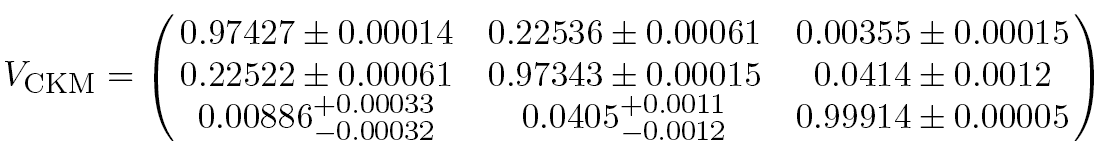
\includegraphics[width=1.0\linewidth]{figs/CKM.png}
\caption{The CKM quark mixing matrix.}
\label{figs:CKM}
\end{center}
\end{figure}



\section{Electroweak Symmetry Breaking}
%From pdg
Through the electroweak symmetry breaking mechanism, the mass of the W and Z bosons, and all fermions can be generated in the SM.  
We consider a scalar potenial of the form:
\begin{eqnarray}
\mathrm{ V(\Phi) = m^{2} \Phi^{\dagger} \Phi + \lambda ( \Phi^{\dagger} \Phi )^{2}  }\\
\mathrm{\Phi = \frac{1}{\sqrt{2}} \left( \frac{\sqrt{2} \phi^{+}}{\phi^{0} + ia^{0}}  \right)}
\end{eqnarray}  
where $\Phi$ is the Higgs field.  A plot of this potential can be seen in Figure~\ref{figs:higgspotential}.  
The minimum of the potential is not at V(0), and this point is unstable.  
The Higgs field has a non-zero vacuum expectation value (VEV).

\begin{figure}
\begin{center}
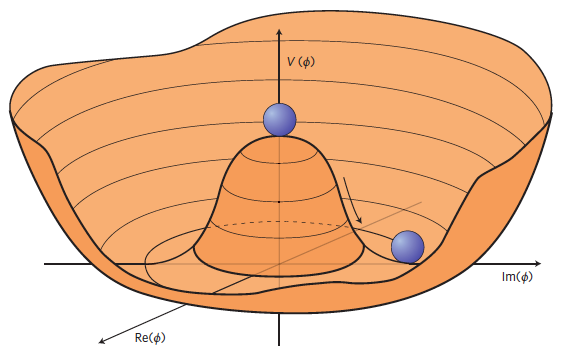
\includegraphics[width=0.7\linewidth]{figs/higgspotential.png}
\caption{The Higgs potential..}
\label{figs:higgspotential}
\end{center}
\end{figure}

Using the Higgs Lagrangian
\begin{eqnarray}
\mathrm{\cal(L) = (D_{\mu} \Phi )^{\dagger}(D_{\mu} \Phi ) -V( \Phi )}\\
(D_{\mu}\Phi) = (\partial_{\mu}+i g \sigma^{\alpha} W_{\mu}^{\alpha}/2 +i g^{'} Y B_{\mu}/2)\Phi
\end{eqnarray}  
we can extract the masses of the W and Z bosons as

\begin{eqnarray}
M_{W}^2 = \frac{g^{2}v^{2}}{4}\\
M_{Z}^2 = \frac{(g^{'2}+g^{2})v^{2}}{4}
\end{eqnarray}  

One new particle is predicted, a massive chargeless spin 0 particle called the Higgs boson.  
A particle consistent with the Higgs boson has been discovered in 2012 at the LHC.  
%https://cds.cern.ch/record/1638469/plots

  
\section{Beyond the Standard Model}
The SM is possibly the most successful theory in physics, but also one that is ultimately incomplete.  
We know that there are physical phenomena that the SM does not predict.  
The presence of dark matter and dark energy in the universe~\cite{Bennett:2003ba} is not currently explained by the SM.  
Given that dark matter and energy account for approximately 95\% of the universe, this is not a small issue.  
The SM does not explain the observation of neutrino oscillations~\cite{An:2012eh}, which implies that neutrinos have mass.  
The SM also does not naturally explain the relative values of fundamental constants such as why the weak force is $10^{33}$ times as strong as gravity.  
This issue is known as the hierarchy problem, and it is assumed that a complete theory would have a natural explanation for the seemingly random values of these constants.  

It is essential for a complete understanding of the universe that we probe beyond the standard model (BSM) theories that provide solutions to these issues.  
Theories involving compact extra dimensions~\cite{PhysRevD.64.035002} for example provide a natural explanation to the hierarchy problem.  
In these theories forces propegate in higher dimensions that are compactified.   
In this theory, the propagation of SM massive fields in higher dimensions leads to discrete modes, which are detectable as new massive particles.  
The propagation of the SM W or Z leads to excited modes that are referred to as the $\wpr$ and $\zpr$.
A novel way to look for BSM physics then is to attempt the creation and detection of massive states such as these bosons. 
In this thesis we discuss one such search for a W' boson.  

The W' boson is a particle predicted by many BSM theories such as Little Higgs~\cite{doi:10.1146/annurev.nucl.55.090704.151502}, 
Composite Higgs models~\cite{Vecchi:2013bja}, and Noncommuting Extended Technicolor~\cite{Chivukula:1995gu}.  





\chapter{Experimental Setup}
\label{sec:ExpSetup}
\chaptermark{Experimental Setup}
One way to search for BSM physics is to produce new particles directly.  
For this, we collide lighter particles at a high energy.  
The energy released in the collision can manifest in more massive particles\footnote{In SUSY there will usually be two} via mass-energy equivalence (E=m$\mathrm{c^2}$).
The collision may create one or more of these new particles, and from it's decay products an experimenter can reconstruct the properties of the new BSM massive state 
and study the properties (mass, decay width, spin, SM couplings etc.).  

For the measurements presented in this thesis, we collide high energy proton beams,  
which are designed to produce a high collision energy in comparison to fixed-target or electron-positron collisions.    
   
\section{Luminosity and Cross Section}
\label{sec:LumiXsec}
To understand how many occurrences of any physical process to expect in a set of collisions, we need to define at a minimum the concepts of luminosity, L, and cross section, $\sigma$.

The cross section of a process is a measure of the probability that a collision will produce the particles of interest.  
The phrase cross section refers to the physical cross section of a classical target and is thus measured in units of area.  
In a high energy collision, the cross section no longer refers to the physical dimensions of the target, and can be calculated directly from Feynman diagrams.  
The areas associated with these cross sections is very small and is measured in barns (b), which is $10^{-28} m^2$.  
BSM physics signatures have cross sections that are generally on the order of picobarns (pb) or femptobarns (fb).  
The process cross section is highly dependent of the energy of the collision and is why it is very important to have large, high energy accelerators for the discovery of new physics.  
The cross section of some SM processes are shown in Figure \ref{figs:SMxsecs}.


\begin{figure}
\begin{center}
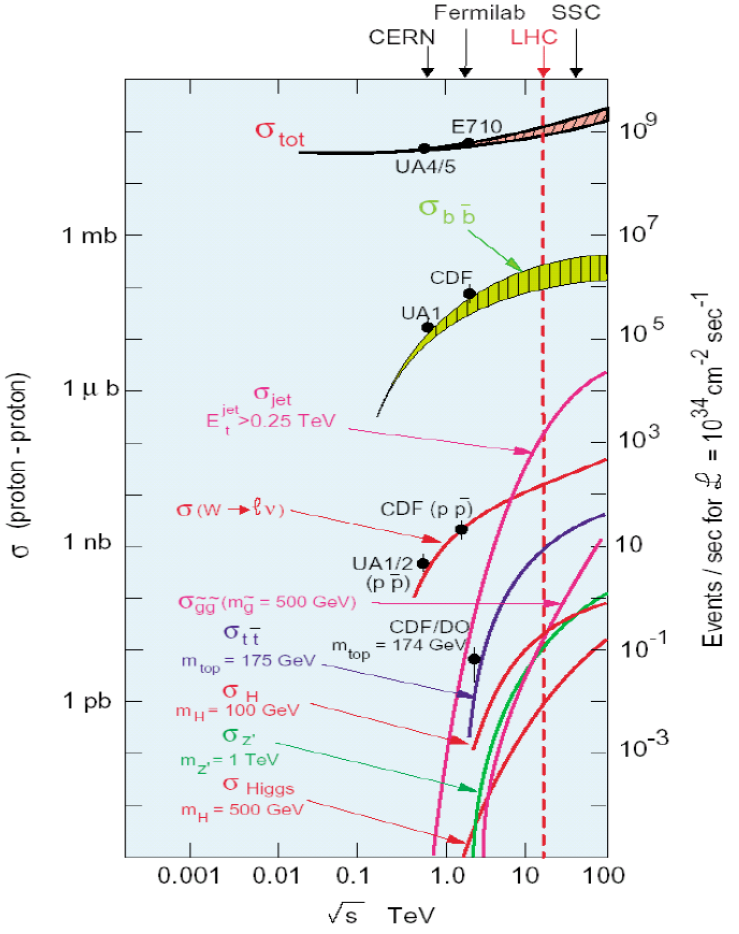
\includegraphics[width=0.7\linewidth]{figs/SMxsecs.png}
\caption{Standard model cross sections as a function of collision energy.}
\label{figs:SMxsecs}
\end{center}
\end{figure}


  
Luminosity is a measure of the intensity of the colliding beams and is the number of collisions expected per unit time per unit area.  
To look for BSM physics, we need to collect an ensemble of useful collisions (events), and thus higher luminosity leads to a larger 
ensemble, and consequently higher statistical precision of the measurement .  
Additionally, collecting data over time leads to a larger ensemble, so the time-integrated luminosity is a more useful variable to describe the total amount of data collected, 
which is reported in $\fbinv$.  Given in relevant collider properties, the luminosity can be defined as~\cite{Bayatian:922757}: 
\begin{eqnarray}
\mathrm{L = \frac{\gamma f k_{B} N_{p}^{2}}{4 \pi \epsilon \beta^{*}} F}
\end{eqnarray}  
where $\gamma$ is the Lorentz factor,  f is the frequency of revolution, $k_{B}$ is the number of bunches in the beam, $N_{p}$ is the number of protons per bunch, 
$\epsilon$ is the transverse emittance, $\beta^{*}$ is the betatron function, and F is a reduction factor based on the crossing angle.  

With these two concepts we can extract the predicted number of events, $N_{\mathrm{i}}$, for a given process i: 
\begin{eqnarray}
N_{\mathrm{i}} = \int L \mathrm{d}t \times \sigma_{\mathrm{i}} 
\label{eqn:Nevents}
\end{eqnarray}  

\section{The LHC}
The Large Hadron Collider (LHC) is a particle accelerator designed to reach collisions energies far surpassing any previous design.  
The LHC is a synchrotron that accelerates protons to 99.999997\% the speed of light.  
These protons beams are then collided at a center-of-mass energy ($\sqrt{s}$) of 8 $\TeV$.  
The accelerator segments and detectors at the LHC are shown in Figure~\ref{figs:lhc}.

% http://home.web.cern.ch/about/accelerators
% http://cds.cern.ch/record/1165534/files/CERN-Brochure-2009-003-Eng.pdf

A proton at the LHC starts out as hydrogen gas within the injector of LINAC 2 linear accelerator.  
The atoms are ionized using an electric field, stripping the electron.  
The resulting proton is accelerated using an oscillating electric field.  
The protons are accelerated in a straight line to an energy of 50~$\MeV$, or 31\% the speed of light.  

At this energy, linear acceleration is not practical, and the protons enter the Proton Synchrotron Booster (PSB).  The PSB is composed of four 157 m 
circumference superimposed synchrotrons that accelerate the protons using electric fields that are synchronized to the revolution frequency of the beams.  
The protons are kept on the circular accelerator with a magnetic field directed into the plane formed by the accelerator ring, which increases in strength as the protons gain energy.  
After the acceleration from the booster, the protons are at en energy of 1.4~$\GeV$, or 92\% the speed of light.

After the PSB, the protons enter the Proton Synchrotron (PS), a 628 m circumference synchrotron, which accelerates the protons to 25~$\GeV$, or 99.93\% the speed of light.  
After the PS, the protons enter the Super Proton Synchrotron (SPS), a 7 km circumference synchrotron, which accelerates the protons to 450~$\GeV$, or 99.9998\% the speed of light.

Finally, the beams enter the LHC.  This is the final synchrotron ring, with a circumference of 27 km.  
After the SPS, the protons are inserted into the LHC in one of two evacuated tunnels depending on which direction around the ring the beam is to travel.  

The LHC uses 1232 dipole magnets to keep the protons in the ring as they accelerate. which provide an 8.3 T field over their length.  
In order to deliver such a field, the magnets use superconducting niobium-titanium cables.  
These cables are cooled by superfluid helium to -271.3 C in order to achieve this superconductivity.  
During each revolution the energy of each proton in the LHC ring increases by 5 MeV.  
After being fully accelerated in the LHC, the protons are at an energy of 4~$\TeV$, or 99.999997 \%the speed of light.

The proton beams are then directed together for collisions in four positions around the ring.  
Each beam in the LHC ring contains 2808 bunches of protons, and each bunch contains 110 billion protons. 
These bunches need to be collimated in order to maximize collision frequency, which is accomplished by the use of 392 focusing quadrupole magnets.   
Each of these collision points houses its own detector, ALICE (A Large Ion Collider Experiment), ATLAS (A Toroidal LHC Apparatus), 
CMS (Compact Muon Solenoid), and LHCb (Large Hadron Collider beauty).  
The ALICE detector is primarily used for experiments involving heavy ion collisions that expand the current 
understanding of concepts such as the quark-gluon plasma and quark confinement   
LHCb is specialized for physics involving b quarks, such as measuring CP violation parameters from b-hadron interactions.  

CMS and ATLAS are large general purpose detectors.  
These detectors are used for many different types of physics searches, and are the two detectors responsible for the Higgs boson discovery.  
For the purposes of this thesis we will be concentrating on the CMS detector
  


\begin{figure}
\begin{center}
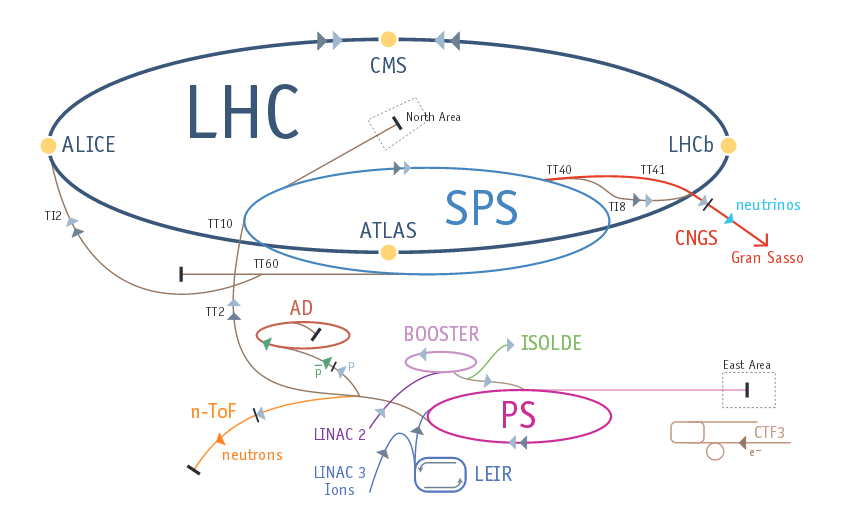
\includegraphics[width=1.0\linewidth]{figs/lhc.png}
\caption{A diagram of the LHC~\cite{lhcbrochure}.}
\label{figs:lhc}
\end{center}
\end{figure}
%http://cds.cern.ch/record/1092437/files/CERN-Brochure-2008-001-Eng.pdf

\section{CMS detector}
Here we will detail the basics of the CMS detector subsystems, for a more complete description, see Reference \cite{Bayatian:922757}.
The purpose of the CMS detector is to measure properties of particles that are created in a collision such as the energy and trajectory. 
The detector needs to collect enough information so that particles can be reconstructed and classified.  
Generally, we can reconstruct most physics signatures by analyzing electrons, muons, photon, charged hadrons, and neutral hadrons. 
The CMS detector has dedicated algorithms and systems that are specifically designed to identify each of these categories.  In order to reconstruct these particles, we impose a uniform axial magnetic field throughout the inner detector with the use of a superconducting magnet. 

The trajectory of charged particles is important for extracting information such as charge and momentum.  
The process of reconstructing the trajectory of these  particles is called tracking.  
Near the interaction point tracks are very dense, and tracking becomes very difficult.  
In this region we use a fine array of silicon pixels that register a charge particles position based on charge deposited in the device.  
Additional measurements are made by a second series of silicon detectors called the Silicon Strip Tracker. 
Using a series of these position measurements, we can fit a charged particle track.  

Energy can be measured by the use of calorimeter systems.  
A calorimeter is a detector designed such that a particle will deposit all of its energy within its volume in the form of photons, 
which can be detected to extract a measure of the total energy. 
These systems are subdivided into the Electromagnetic Calorimeter (ECAL) and Hadronic Calorimeter (HCAL).  
The ECAL uses scintillation crystals to detect particles that interact primarily with the electromagnetic force such as electrons and photons.  
Hadrons pass through the ECAL with minimal loss and deposit energy in the HCAL, which uses layers of absorber and scintillator to first 
create a shower of secondary particles, and then measure the total energy of these secondary particles.  

The detection of muons requires a specially designed system that lies outside of the ECAL, HCAL, and magnet.  
Muons pass through the ECAL and HCAL without losing a substantial fraction of their energy.  
To reconstruct the trajectory of muons, we use several different systems both inside and outside the magnet.

See Figure~\ref{figs:CMSdiagram1} for a diagram of the full detector, and Figure~\ref{figs:CMSdiagram} for a cross-sectional view of the detector subsystems.

\begin{figure}
\begin{center}
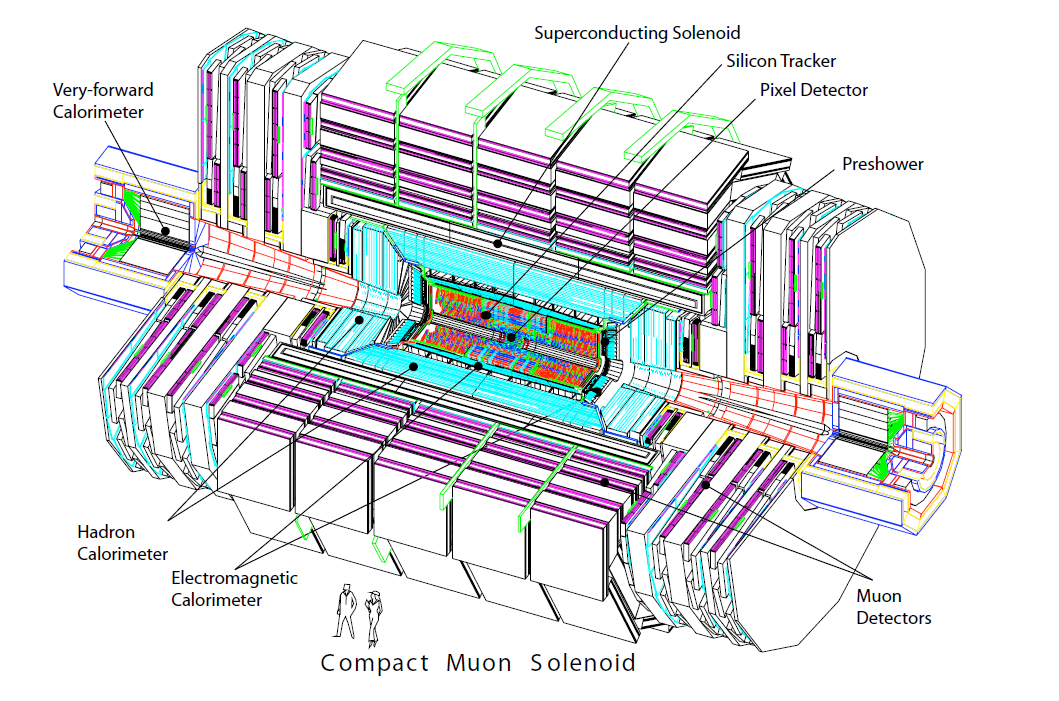
\includegraphics[width=1.0\linewidth]{figs/CMSdiagram1.png}
\caption{A diagram of the full CMS detector.}
\label{figs:CMSdiagram1}
\end{center}
\end{figure}

\begin{figure}
\begin{center}
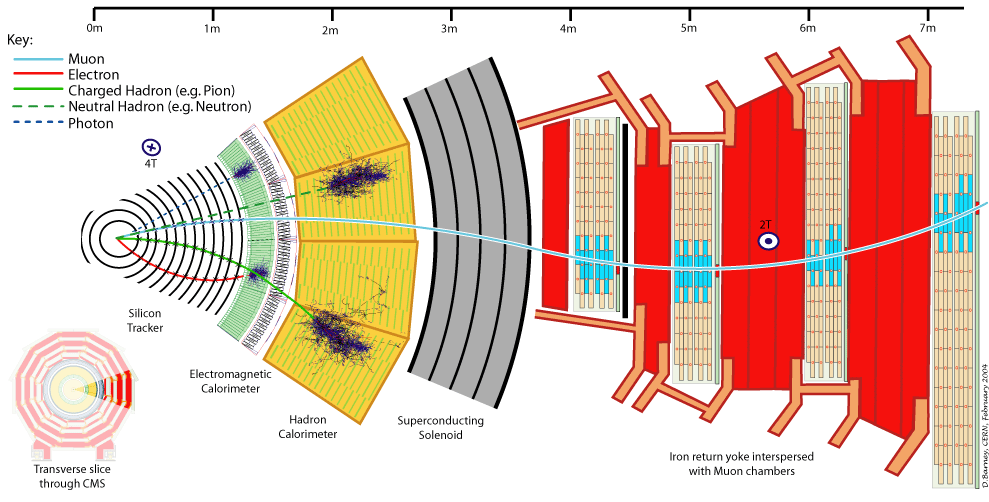
\includegraphics[width=1.0\linewidth]{figs/CMSdiagram.png}
\caption{A cross-sectional view of the CMS detector.}
\label{figs:CMSdiagram}
\end{center}
\end{figure}



\subsection{Pixel Tracker}
The closest detector system to the interaction point is the silicon pixel tracking system (see Figure \ref{figs:CMSpixel}).   .  
This system extends from a radius of 4 cm to 11 cm in the barrel, and is designed to track charged particles in a very dense environment.  
This is achieved with three arrays of two dimensional silicon pixels placed at a radii of 4.4 cm, 7.3 cm, and 10.2 cm, as well as two endcap disks for a total of 65 million pixels.  
When a charged particle traverses one of the 100 $\mum$ $\times$ 150 $\mum$ pixels, it imparts enough energy to the silicon to eject an electron.  
The electrons and their corresponding hole are detected on the pixel surface as a signal.  
This signal allows us to extract a position measurement for the charged particle.  

The entire system exists in a magnetic field, so the trajectory of the electrons and holes are deflected in the r,$\phi$ plane before detection.  
The angle of this Lorentz drift is 23$\textdegrees$, which causes the electron-hole pairs to be detected over a wide region covering multiple pixels.  
This effect improves the spacial resolution to 10 $\mum$ in r-$\phi$ space due to the fact that the charge center can be reconstructed by more measurements, 
whereas the z resolution is 20 $\mum$ due to the fact that there is no magnetic deflection in this direction. 
The pixel detectors in the endcap disks are angled at 20$\textdegrees$ in a turbine-like design to take advantage of this effect.  

  

\begin{figure}
\begin{center}
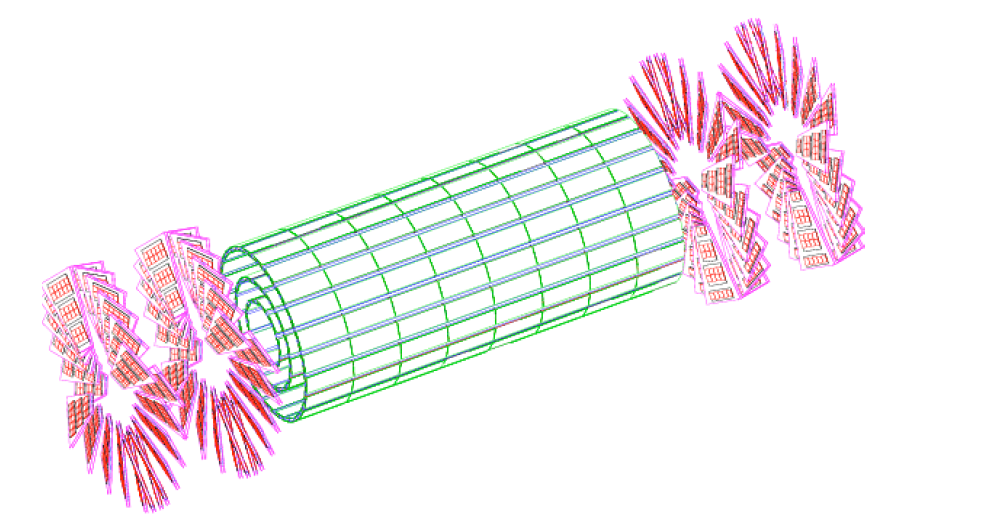
\includegraphics[width=1.0\linewidth]{figs/CMSpixel.png}
\caption{A diagram of the pixel detector.}
\label{figs:CMSpixel}
\end{center}
\end{figure}
  
\subsection{Silicon Strip Tracker}
Outside of the silicon pixel tracker (see Figure \ref{figs:CMStracker}) out to a radius of 130 cm in the barrel lies the silicon strip tracking system.  

The system in segmented into the inner barrel, outer barrel, inner disk, and endcap segments.  
The inner barrel segment (20 cm $<$ r $<$ 55 cm) uses four arrays of 10 cm $\times$ 80 $\mum$ silicon microstrips .  
The outer barrel (55 cm  $<$ r $<$ 130 cm) uses six arrays of large pitch 25 cm $\times$ 180 $\mum$ silicon microstrips.  

The endcap silicon strip detector consists of nine disks from 120 cm  $<$ z $<$ 280 cm.  
The inner disk segment contains three smaller disks that connect the inner barrel and endcap segments.  

\begin{figure}
\begin{center}
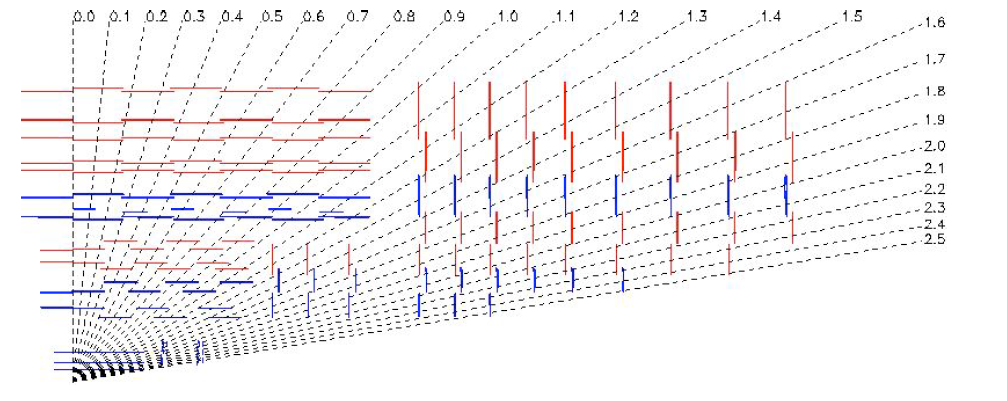
\includegraphics[width=1.0\linewidth]{figs/CMStracker.png}
\caption{A diagram of the silicon tracking system.}
\label{figs:CMStracker}
\end{center}
\end{figure}
  


%\subsection{Preshower Calorimeter}
\subsection{Electromagnetic Calorimeter}
The ECAL (see Figure~\ref{figs:CMSecal}) is designed to provide energy information for electrons and photons.  
These particles will typically deposit all of their energy within the detector, which is detectable as photons. 

To do this, the ECAL uses 61200 lead tungstate ($\mathrm{PbWO_4}$) scintillation crystals in the barrel and 7324 in each endcap.  
Lead tungstate is chosen as a scintillation material because it has a short radiation length (0.89 cm), fast response (25 ns for 80\% of light), and can 
withstand harsh radiation environments (10 Mrad).
The light emitted is around 30 photons per $\MeV$ for the energy of the particle of interest, which is somewhat low.  
Therefore, the ECAL uses avalanche photodiodes in the barrel and voltage phototriodes in the endcap segments to amplify the signal upon readout.  

The endcap regions of the ECAL include a preshower detector that is used to distinguish high energy photons from decaying pions.  
A pion decaying to two closely spaced photons can mimic one high energy photon to the 2.2 cm wide ECAL crystals.  
The preshower is able to distinguish these events with a finer granularity (2 mm) silicon strip detector.   
 
\begin{figure}
\begin{center}
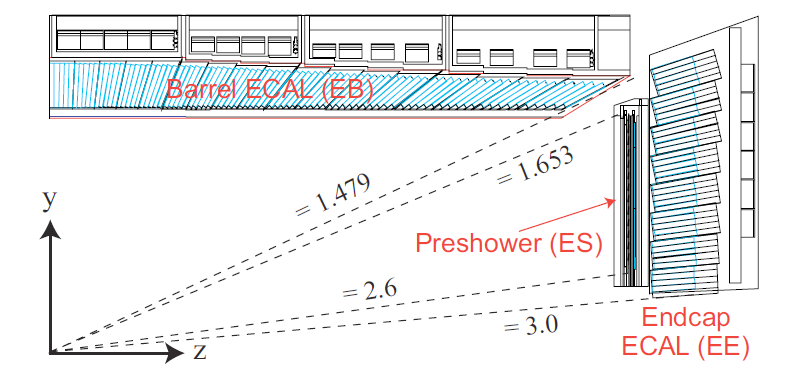
\includegraphics[width=1.0\linewidth]{figs/CMSecal.png}
\caption{A diagram of the ECAL system.}
\label{figs:CMSecal}
\end{center}
\end{figure}
  





\subsection{Hadronic Calorimeter}
The HCAL (see Figure~\ref{figs:CMShcal}) is designed to give the energy of charged and neutral hadrons, which generally lose very little energy in the ECAL.  
The HCAL is segmented into the inner barrel (inside the magnet), outer barrel (outside the magnet), endcap, and forward (close to the beamline).  

The HCAL uses alternating layers of absorber and scintillator to calculate the energy of these hadrons.  
The absorber creates a cascade of secondary particles that emit photons in the scintillator which can then be detected and summed to reconstruct the energy of the initial hadron.  
The photons emitted in the scintillator are carried to the photodetectors by optical waveguides.  
The HCAL uses hybrid photodiodes to detect the scintillation light and provide a signal that can be used to extract the total energy of the hadron.  

\begin{figure}
\begin{center}
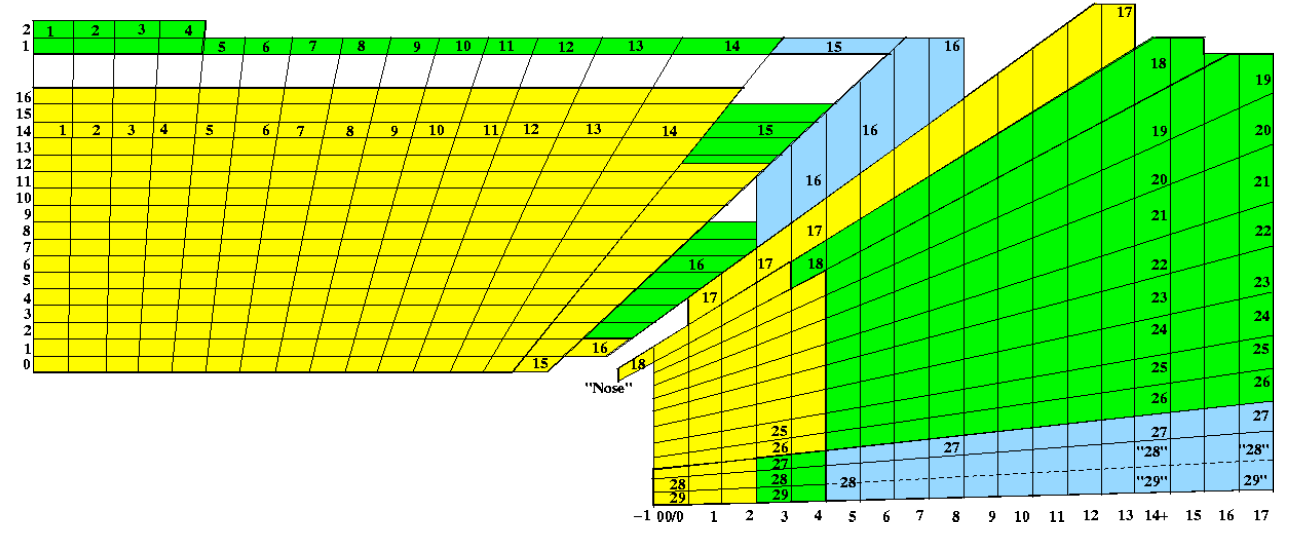
\includegraphics[width=1.0\linewidth]{figs/CMShcal.png}
\caption{A diagram of the HCAL system.}
\label{figs:CMShcal}
\end{center}
\end{figure}
  
\subsection{Magnet}
A charged particle moving perpendicular to a magnetic field follows a helical trajectory.  
The curvature of this helix is dependent on the momentum of the particle, and the handedness is dependent on the charge.  
Therefore, by immersing the tracking volume in an axial magnetic field we can get an accurate measurement of these properties.  
The stronger the magnetic field, the more precise these measurements can be for a high energy particle due to the more distinct curvature.  
To produce this field, CMS employs the largest superconducting magnet ever built.  

The design goal for the magnet is to be able to reproduce high momentum muons.  
The benchmark used for this is to have a momentum resolution of $\Delta$p/p $\leq$ 10\% at a muon momentum of 1 $\TeV$.  
To achieve this, we employ a solenoid with a length of 12.9 m and bore of 5.9 m.  
The coils of this solenoid are superconducting niobium-titanium, which produce a uniform 3.8 T magnetic field in the interior. 
The coils are wound in four layers, for a total of 2168 turns that carry 19.5 kA of current.    

The magnet additionally provides structural support to withstand the weight of the CMS detector as well as the magnetic force exerted from it's own magnetic field.  

\subsection{Muon System}
The reconstruction of muons and electrons starts at the inner silicon tracking system.  
Whereas electrons deposit their energy in the ECAL, a muon will traverse the ECAL and HCAL without significant interaction because a muon is around 200 times as massive.  
Muons are of interest to the Higgs discovery as well as BSM physics, 
and an accurate determination of the muon energy is also required for determination of the total event energy and missing energy.  
Therefore, the CMS detector has a large system purely designed to reconstruct muons, which lies outside all other detector systems at CMS.  

The muon system is comprised of a gaseous detectors interleaved with iron.  
The iron is saturated with the return field of the magnet, which creates a magnetic field at one half of the internal field strength and oriented in the opposite direction.  
The three layers of this ``return yoke" system bends muons to get an accurate measure of the momentum outside of the magnet.  

The trajectory of the muons is reconstructed with three types of gaseous detectors.  
The detectors work on the same basic principle, where an incoming muon ionizes the gas creating an electron-hole pair.  
The electron is detected by the anode, and the hole is detected by a cathode.  
A coincidence of these two measurements gives a measure of the position and time that a muon traversed the detector.  
With a series of these measurements, a trajectory can be fit, and physical quantities of interest can be reconstructed.  

In the barrel region ($|\eta|$ $<$ 1.2), drift tubes are used because the neutron flux and magnetic field are low.  
A drift tube is a detector consisting of a gas filled tube with an anode wire.  
The ionized electron from the gas volume travels to the anode wire, and a measurement of position is made.  
The detection of this electron registers the position along the wire (z coordinate).  
The r-$\phi$ coordinate within the drift tube cross sectional can be calculated by using the drift time of the ionized electrons to the anode.  

In the endcap region, where the magnetic field and neutron flux are high, cathode strip chambers are used.  
Cathode strip chambers are trapezoidal in shape with six gas gaps for ionization.  
These gas gaps each have one plane of cathode strips pointing radially outward and one plane of anode wires oriented perpendicular to the cathode.  

In both the barrel and endcap regions, resistive plate chambers are used.  
These detectors are composed of two parallel resistive plates separated by a gas gap.  
The design goal of the resistive plate chambers is to complement the cathode strip chambers and drift tubes to give two independent measurements of position.  
Additionally, resistive plate chambers offer very quick and accurate time resolution.  This offers a 
quick approximation of the muon momentum which is useful for the trigger system and matching a muon track to a bunch crossing.  

The muon system and inner tracker both contribute to the trajectory measurement of a muon.  
In terms of momentum resolution, the inner tracker offers much better sensitivity up to around 200 $\GeV$.  
After 200 $\GeV$, the muon system starts to significantly improve the momentum measurement.

Figure \ref{figs:CMSmuon} shows a diagram of the muon system.  
\begin{figure}
\begin{center}
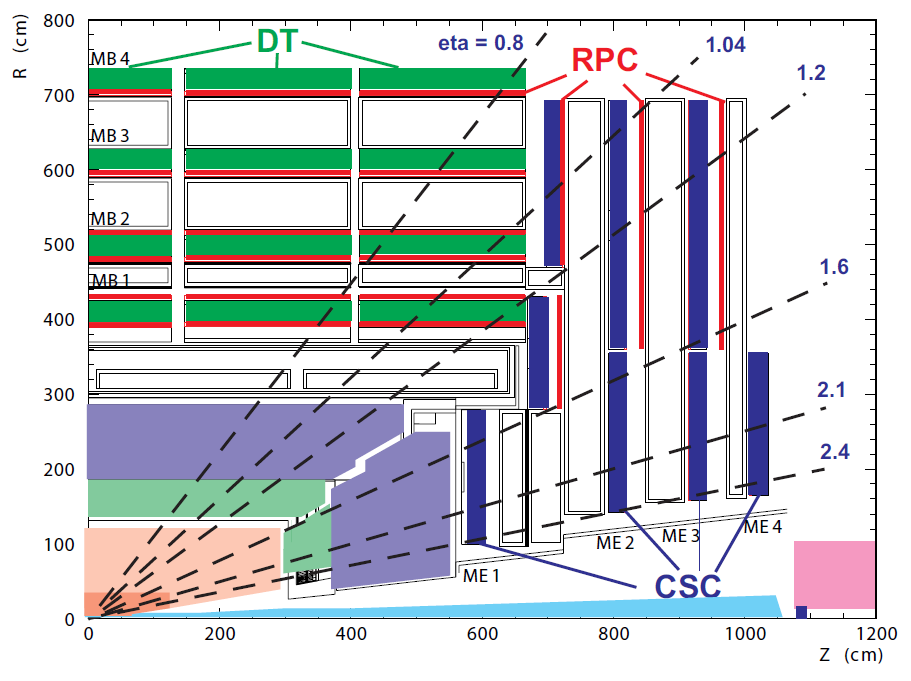
\includegraphics[width=1.0\linewidth]{figs/CMSmuon.png}
\caption{A diagram of the muon system.}
\label{figs:CMSmuon}
\end{center}
\end{figure}

\subsection{Trigger}
The LHC delivers around 1 billion proton-proton collisions per second.  
However, because of the current computing limitations, the CMS detector system can only write around 100 collisions per second as data.  
Therefore, a trigger system is developed to distinguish the most potentially interesting physics signatures.  

The L1 trigger takes information from the calorimeter and muon systems and their correlations.  
When one of these detectors produces a signal, the information takes 3.2 $\mus$ to reach the L1 processing area and return to the detector.  
The L1 processing time for the information for a maximum of 1 $\mus$ where the decision is made to keep the event to search for potential physics signatures.  
The L1 has various algorithms designed to keep ``trigger primitives", which can be objects such as high $\pt$ muons, electrons, jets or full event information like total energy or $\MET$.  
The L1 trigger only saves on average of 1 out of every 1000 events.  

After the L1 trigger, the trigger primitive events are processed by the high level trigger (HLT).  
The HLT again saves only 1 out of 1000 of these events.  
The processing time for the HLT algorithm is longer than the L1 system, and to extract the potentially exciting physics objects the algorithm performs partial event reconstruction.  
An event that enters the HLT algorithm is first analyzed based on the output of the calorimeters and muon system, then pixel tracking is performed, then finally full tracking.  
An event that passes the L1 and HLT is then put into storage for analysis.  

%\subsection{Computing Grid}



\chapter{Higgs Phenomenology at the LHC}
\label{sec:HiggsPhen}
\chaptermark{Higgs Phenomenology at the LHC}

In the simplest incarnation of the Higgs mechanism, the Higgs boson
mass is the only free parameter.  Given the mass of the Higgs 
boson, the production cross section, branching fractions, and 
decay width can be calculated.
Generally, the Higgs boson 
couples most strongly to the most massive particles in the 
SM.  However, the mechanism for which the weak gauge 
bosons acquire mass and the fermions acquire mass in the SM is 
different.  
Thus, the coupling of the Higgs boson to fermions is proportional 
to the mass of the fermion while the coupling of the 
Higgs boson to the weak gauge bosons is proportional to the square 
of the gauge boson's mass. These features and the structure 
functions of the proton combine to produce the predictions shown in 
Figure~\ref{fig:HiggsProdXS} for the production cross-section and 
branching fraction of the Higgs.  

\begin{figure}
\begin{center}
\includegraphics[width=.56\linewidth]{HiggsPhenPlots/Higgs_XS_8TeV.eps}
\includegraphics[width=.42\linewidth]{HiggsPhenPlots/Higgs_BR.eps}
\caption{left: Higgs production cross section vs $m_H$ for 
different processes at $\sqrt{s}=8~TeV$. right: Higgs branching
ratios vs $m_H$.  Both calculations are taken from the LHC Higgs
cross section working group. }
\label{fig:HiggsProdXS}
\end{center}
\end{figure}

In this chapter, the terminology of the different production and 
decay channels are introduced as well as the experimental 
signatures for each.  Kinematics of spin-0, spin-1, 
and spin-2 resonances decaying to two vector bosons are introduced.  
Techniques for using decay kinematics for increasing signal 
sensitivity and performing property measurements are presented.  

\section{Higgs Signatures}

\subsection{Gluon-gluon Fusion}
\label{sec:ggHiggs}

The gluon-gluon fusion production mechanism is responsible for 
$\sim87\%$ of Higgs events produced at 
the LHC, assuming $m_H=125$~GeV and $\sqrt{s}=8$~TeV.  This is due 
to the gluon-gluon cross 
section dominating over other initial states for the relevant range 
of invariant masses, as shown in Figure~\ref{fig:LHCpdfs}.
However, because the Higgs cannot couple to gluons directly, the
interaction must be mediated through a loop, show in 
Figure~\ref{fig:ggFusion}.  The dominant contributions 
come from the heavy quarks, top and bottom quarks, which couple
strongly to both gluons and the Higgs.  The production cross 
section for this process varies from $3\times10^{-2}~pb$ to $40~pb$
for Higgs masses between 80 and 1000 GeV and $\sqrt{s}=8~TeV$.

\begin{figure}
\begin{center}
\includegraphics[trim=0 0 0 420,clip,width=.7\linewidth]{HiggsPhenPlots/pdf_factor.eps}
\caption{Distribution of parton factor, F(s,Y=0), showing the 
relative probability for producing resonances from gluon-gluon, or 
$q\bar{q}$ interaction.}
\label{fig:LHCpdfs}
\end{center}
\end{figure}

\begin{figure}
\begin{center}
\unitlength=1mm
\begin{fmffile}{ggFusion}

\begin{fmfgraph*}(40,40) \fmfpen{thick}
  \fmfleft{i1,i2} \fmfright{o1}
  \fmf{gluon,label=$g$}{i1,v1} \fmf{gluon,label=$g$}{i2,v2}
  \fmf{fermion,label=$t$}{v1,v2}
  \fmf{fermion,label=$~\bar{t}$}{v3,v1}
  \fmf{fermion,label=$~~~t$}{v2,v3}
  \fmf{dashes,label=$H$}{v3,o1}
\end{fmfgraph*}

\end{fmffile}
\end{center}
\caption{Feynman diagram depicting the leading contribution to 
gluon-gluon fusion production of a Higgs boson.}
\label{fig:ggFusion}
\end{figure}

\subsection{Weak Vector Boson Fusion}
\label{sec:VBFHiggs}

The Weak Vector Boson Fusion (VBF) production mechanism has the next to
largest cross section at the LHC, depicted in Figure~\ref{fig:VBF}.  The 
signature of this production mechanism is two energetic jets at high values 
of pseudorapidity.  Because of gluon radiation from next-to-leading
order (NLO) and next-to-NLO (NNLO) QCD effects, gluon-gluon fusion events can
also have this same signature.  As such, event classes which attempt to 
distinguish the VBF production mechanism tend to have a large contamination 
from gluon-gluon fusion.  Usually the kinematics of the spectator jets
can be used to further isolate VBF-like events. 

\begin{figure}
\begin{center}
\unitlength=1mm
\begin{fmffile}{VBF}

\begin{fmfgraph*}(40,30) \fmfpen{thick}
  \fmfleft{i1,i2} \fmfright{sp1,H,sp2}
  \fmf{fermion,label=$q$}{i1,v1,sp1} 
  \fmf{fermion,label=$q$}{i2,v2,sp2}
  \fmf{photon,label=$V$}{v1,v3}
  \fmf{photon,label=$V$}{v2,v3}
  \fmf{dashes,label=$H$}{v3,H}
\end{fmfgraph*}

\end{fmffile}
\end{center}
\caption{Feynman diagram depicting weak vector boson fusion production
of a Higgs boson.}
\label{fig:VBF}
\end{figure}

\subsection{Other Production Mechanisms}
\label{sec:VHiggs}

Other production mechanisms produce Higgs bosons in association with either
a weak gauge boson or top pair, both of which are depicted in 
Figure~\ref{fig:VHttH}.  In these cases either W or Z can be tagged or the 
presence of 
b-jets can be included.  However, for $m_H=125$~GeV, these processes only make up ~5\% of the 
total Higgs boson production cross section at the LHC.  As such, having 
significant 
sensitivity to these production mechanisms requires very high amount of 
integrated 
luminosity, $\mathscr{O}(100~fb^{-1})$. 

\begin{figure}
\begin{center}
\unitlength=1mm
\begin{fmffile}{VH_and_ttH}

\begin{fmfgraph*}(40,30) \fmfpen{thick}
  \fmfleft{i1,i2} \fmfright{V,H}
  \fmf{fermion,label=$\bar{q}$}{v1,i1}
  \fmf{fermion,label=$q$}{i2,v1}
  \fmf{photon,label=$V^{*}$}{v1,v2}
  \fmf{photon,label=$V$}{v2,V}
  \fmf{dashes,label=$H$}{v2,H}
\end{fmfgraph*}
~
\begin{fmfgraph*}(50,30) \fmfpen{thick}
  \fmfleft{i1,i2} \fmfright{sp1,H,sp2}
  \fmf{photon,label=$g$}{i1,v1}
  \fmf{photon,label=$g$}{i2,v2}
  \fmf{fermion,label=$t$}{v1,sp1}
  \fmf{fermion,label=$\bar{t}$}{v3,v1}
  \fmf{fermion,label=$\bar{t}$}{sp2,v2}
  \fmf{fermion,label=$t$}{v2,v3}
  \fmf{dashes,label=$H$}{v3,H}
\end{fmfgraph*}

\end{fmffile}
\end{center}
\caption{Feynman diagram depicting associated production (left) and $t\bar{t}$ 
fusion production of a Higgs boson.}
\label{fig:VHttH}
\end{figure}

\subsection{Decay Channels}
\label{sec:HiggsDecays}

The partial decay widths of the Higgs boson, just as with productions, are typically related to the mass of the decay products.  As such, at low 
mass, where the production of weak gauge bosons is suppressed from 
phase-space effects, b-quarks are the dominant decay, making up $\sim80\%$ of 
the events.  At high mass, the leading decays are to W and Z pairs.  
The SM has the particular feature that the $H\to\gamma\gamma$ and 
$H\to Z\gamma$ branching ratios are much smaller than the $H\to ZZ$ or 
$H\to WW$ branching ratios
because the Higgs does not couple directly to massless particles.  Thus, these
processes are required to proceed through loops which would contain massive
particles, usually either top quarks or W bosons.  This is one of the 
most distinguishing features which results in a large suppression of 
the $\gamma\gamma$ and $Z\gamma$ channels with respect to the ZZ and WW
channels.  The branching ratios versus $m_H$ are shown in 
Figure~\ref{fig:HiggsProdXS} for different decay channels. 

Because of the distinct signature of ZZ,
WW, and $\gamma\gamma$ decays, these channels are the most sensitive for 
discovering a Higgs-like resonance.  The $4\ell$ final state of the ZZ 
channel is especially promising because it is a high resolution, fully 
reconstructable channel with very small SM backgrounds.


\section{Kinematics of Scalar Resonances}
\label{sec:Kinematics of scalar resonances}

The simplest incarnation of the Higgs mechanism predicts one scalar 
boson with the simplest coupling to the SM fields.  However, there 
are models which go beyond the minimal Higgs mechanism and predict 
other scalars which would couple differently to the SM fields.  
The most generic amplitude for a scalar which couples to two 
bosons is
\begin{equation}
\begin{split}
  \mathscr{A}(X\to VV) = v^{-1}(g_1m_v^2\epsilon_1^*\epsilon_2^*+g_2f_{\mu\nu}^{*(1)}f^{*(2),\mu\nu}+ \\
g_3f^{*(1),\mu\nu}f_{\mu\alpha}^{*(2)}\frac{q_\nu q^\alpha}{\Lambda^2}+g_4f_{\mu\nu}^{*(1)}\tilde{f^{*(2),\mu\nu}}),
\label{eq:scalarAmp}
\end{split}
\end{equation}
where $f$ and $\tilde{f}$ are the field strength tensor and the 
conjugate field strength tensor, $g_i$ are dimensionless couplings,
$\epsilon_i$ are the polarization vectors of the vector bosons, 
$\Lambda$ denotes the scale where new physics could appear, $m_V$ 
is the mass of the vector boson, and q is the momentum of the 
VV-system.  This amplitude corresponds to three independent
Lorentz structures and can be rewritten as,
\begin{equation}
\mathscr{A}(X\to VV) = v^{-1}\epsilon_1^{*\mu}\epsilon_2^{*\nu}(a_1g_{\mu\nu}m_X^2+a_2q_\mu q_\nu+a_3\epsilon_{\mu\nu\alpha\beta}q_1^{\alpha}q_2^{\beta}). 
\label{eq:masterEq}
\end{equation}
The translation between the couplings used in Equation~\ref{eq:scalarAmp} and those used in Equation~\ref{eq:masterEq} can be found in Equation 12 of Reference~\cite{Bolognesi:2012mm}.  The SM Higgs boson couples to the weak vector boson only through the $a_1$ term and
couples to photons through an effective coupling which is a 
combination of the $a_1$ and $a_2$ terms.  A CP-odd scalar, 
commonly referred to as a pseudoscalar, couples to the gauge 
bosons through the $a_3$ term.

The amplitude can be broken into several more specific amplitudes, 
known as helicity amplitudes, corresponding to the helicity states 
of the vector bosons, where the quantization axis is taken to be 
the direction of the VV decay in the resonance's rest frame.  For 
a scalar resonance, there are only three non-zero helicity 
amplitudes out of the nine permutations,
\begin{center}
\begin{subequations}
  \begin{equation}
    A_{00} = -\frac{m_X^2}{v}\left(a_1\sqrt{1+x}+a_2\frac{m_1m_2}{m_X^2}x\right),    \end{equation}
  \begin{equation}
    A_{++} = \frac{m_X^2}{v}\left(a_1+ia_3\frac{m_1m_2}{m_X^2}\sqrt{x}\right),
    \end{equation}
  \begin{equation}
    A_{--} = \frac{m_X^2}{v}\left(a_1-ia_3\frac{m_1m_2}{m_X^2}\sqrt{x}\right),
    \end{equation}
\end{subequations}
\end{center}
where $x$ is defined as
\begin{equation}
x=(\frac{m_X^2-m_1^2-m_2^2}{2m_1m_2})^2-1.
\end{equation}

While the above formulas apply to all bosonic decays of 
scalar resonances, $ZZ\to4\ell$ decays are particularly well 
suited for performing property measurements.  This final 
state has very good momentum and angular resolution, low
SM backgrounds, and sufficient complexity for all features
of the most generic amplitude to be manifested.

A convenient basis of variables which can be
used to fully describe $ZZ\to4\ell$ decays in the ZZ rest frame 
consists of the three invariant masses ($m_{ZZ}$, $m_Z$, and 
$m_Z^*$) and 5 angles, depicted in Figure~\ref{fig:HZZdiagram}.
Each helicity amplitude has a distinct angular distribution while
the magnitude of each helicity amplitude depends on the invariant
masses of the two Z bosons and the resonance.  Together these 
combine into the differential cross section according to
\begin{equation}
\begin{split}
\mathscr{P}(m_1,m_2,\vec{\Omega})\propto|P_V(m_1,m_2)|  \\
\times\frac{m_1^3}{(m_1^2-m_V^2)^2+m_V^2\Gamma_V^2}\times\frac{m_2^3}{(m_2^2-m_V^2)+m_V^2\Gamma_V^2} \\
\times\frac{d\Gamma_J(m_1,m_2,\vec{\Omega})}{d\vec{\Omega}},
\end{split}
\end{equation}
where q is the magnitude of the vector boson momentum in the resonance's rest-frame.
For a spin-0 resonance, the angular distributions are given 
by
\begin{equation}
\begin{split}
\frac{d\Gamma_{J=0}}{\Gamma d\vec{\Omega}} = 4|A_{00}|^2\sin^2\theta_1\sin^2\theta_2 \\
+|A_{++}|^2(1-2A_{f1}\cos\theta_1+\cos^2\theta_1)(1+2A_{f2}\cos\theta_2+\cos^2\theta_2)\\
+|A_{--}|^2(1+2A_{f1}\cos\theta_1+\cos^2\theta_1)(1-2A_{f2}\cos\theta_2+\cos^2\theta_2)  \\
+4|A_{00}||A_{++}|(A_{f1}+\cos\theta_1)\sin\theta_1(A_{f2}+\cos\theta_2)\sin\theta_2\cos(\Phi+\phi_{++}) \\
+4|A_{00}||A_{--}|(A_{f1}-\cos\theta_1)\sin\theta_1(A_{f2}-\cos\theta_2)\sin\theta_2\cos(\Phi-\phi_{--}) \\
+2|A_{++}||A_{--}|\sin^2\theta_1\sin^2\theta_2\cos(2\Phi-\phi_{--}+\phi_{++})
\end{split}
\label{eq:angularDist}
\end{equation}
where $A_{fi}$ are the $Z\to f\bar{f}$ amplitudes which can be
found in Reference~\cite{Bolognesi:2012mm}.
The resulting differential cross section is parameterized in terms of 
the underlying couplings. 
The angular and mass distributions for several types of scalar 
models are shown in Figures~\ref{fig:ScalarMasses} 
and~\ref{fig:ScalarHelicityAngles}.  The red and blue distributions
correspond to a SM Higgs and pseudoscalar resonances.  The green 
distributions correspond to a scalar model in which the resonance couples
to the vector boson only through the $g_2$ term of 
Equation~\ref{eq:scalarAmp}, referred to here as
the $0_{h}^+$ model.  Thus, these three models 
represent the three independent Lorentz structures of the most generic
scalar-vector-vector amplitude.  

\begin{figure}
\begin{center}
\includegraphics[width=.49\linewidth]{FutureMeasurementsPlots/angles-HZZ4l_snowmass.eps}
\caption{Diagram depicting $H\to ZZ\to4\ell$ decays and definition
of angles which describe the kinematics of these decays.}
\label{fig:HZZdiagram}
\end{center}
\end{figure}

\begin{figure}
\begin{center}
\includegraphics[width=.32\linewidth]{HiggsPhenPlots/spinParityPaper/plots/z1mass_125GeV_spin0_3in1.eps}
\includegraphics[width=.32\linewidth]{HiggsPhenPlots/spinParityPaper/plots/z2mass_125GeV_spin0_3in1.eps}
\caption{Distributions of the Z boson masses.  The smaller of the two masses is
plotted on the right, while the larger of the two masses is plotted on the
left. Markers show simulation of events using JHUGen; lines are projections
of the analytical distribution described above.  Red lines/circles correspond
to a SM Higgs, blue lines/diamonds, a pseudoscalar, and green lines/square, 
a CP-even scalar produced from higher dimension operators.}
\label{fig:ScalarMasses}
\end{center}
\end{figure}

\begin{figure}
\begin{center}
\includegraphics[width=.32\linewidth]{HiggsPhenPlots/spinParityPaper/plots/costheta1_125GeV_spin0_3in1.eps}
\includegraphics[width=.32\linewidth]{HiggsPhenPlots/spinParityPaper/plots/costheta2_125GeV_spin0_3in1.eps}
\includegraphics[width=.32\linewidth]{HiggsPhenPlots/spinParityPaper/plots/phi_125GeV_spin0_3in1.eps}
\caption{Distributions of helicity angles, $\cos\theta_1$ (left), 
$\cos\theta_2$ (middle), and $\Phi$ (right). Markers show simulation of 
events using JHUGen; lines are projections
of the analytical distribution described above.  Red lines/circles correspond
to a SM Higgs, blue lines/diamonds, a pseudoscalar, and green lines/square, 
a CP-even scalar produced from higher dimension operators.}
\label{fig:ScalarHelicityAngles}
\end{center}
\end{figure}

In principle,
a mixture of these terms can occur.  In fact, there is a small but 
negligible contribution from the $g_2$ term in the SM from 
higher order electroweak corrections.  In various extensions to the SM, e.g. 
2 Higgs doublet models, multiple scalars exist with different CP 
properties.  It is even possible that CP-violating interactions 
could exist.  
%The distributions in Figures~\ref{fig:ScalarMasses} 
%and~\ref{fig:ScalarHelicityAngles} clearly demonstrate that with 
%enough events, the angular and mass distributions are sufficient to 
%determine the couplings of an observed scalar resonance.  
Constraining the contribution
from either the $g_2$ or $g_4$ term of the amplitude can be more 
aptly 
formulated through a reparametrization of the HZZ amplitude.  
Starting from the three complex couplings, $g_1$, $g_2$, and $g_4$,
four real parameters can be defined
\begin{center}
\begin{subequations}
  \begin{equation}
    f_i = \frac{|g_i|^2\sigma_i }{|g_1|^2\sigma_1+|g_2|^2\sigma_2+|g_4|\sigma_4}
    \end{equation}
  \begin{equation}
    \phi_{gi} = arg(\frac{g_i}{g_1}),
    \end{equation}
\label{eq:HZZmodelParams}
\end{subequations}
\end{center}
for $i=2,~4$. 
In the above formula, $\sigma_i$ is the cross section of the 
process corresponding to $g_i=1$ and $g_{\neq i}=0$.  The $f_{gi}$
parameters represent an effective fraction of events
resulting from the corresponding term of the amplitude.  In the 
case where there is no interference, this interpretation is exact.
This parametrization factorizes out the total cross section,
assuming that it will be measured separately. These variables are 
also straight forward measurables for experiments where rates are 
directly measured, as will be discussed in later sections.  In 
Chapters~\ref{sec:HZZsearches}, a slightly different notation will
be used for the fractions and the translation, $f_{a3}=f_{g4}$ and 
$f_{a2}=f_{g2}$ should be applied.

Similar differential cross sections can be calculated for a generic spin-1 or spin-2 
resonance decaying to two Z bosons~\cite{Bolognesi:2012mm}.  
Figures~\ref{fig:VectorMasses},~\ref{fig:VectorProdAngles}, 
and~\ref{fig:VectorHelicityAngles} show two choice vector 
resonance models.  
Figures~\ref{fig:TensorMasses},~\ref{fig:TensorProdAngles}, 
and~\ref{fig:TensorHelicityAngles}
show three choice tensor 
resonance models.  The couplings used to define each of these 
models are shown in Table~\ref{table:alternativeModels}.  
%Similar 
%to the case of a scalar resonance, sufficient information is 
%contained in the angular and mass distributions to 
%constrain all the parameters of the vector-vector-vector amplitude. 

\begin{figure}
\begin{center}
\includegraphics[width=.32\linewidth]{HiggsPhenPlots/spinParityPaper/plots/z1mass_125GeV_spin1_2in1.eps}
\includegraphics[width=.32\linewidth]{HiggsPhenPlots/spinParityPaper/plots/z2mass_125GeV_spin1_2in1.eps}
\caption{Distributions of the Z boson masses.  The smaller of the two masses is
plotted on the right, while the larger of the two masses is plotted on the
left. Markers show simulation of events using JHUGen; lines are projections
of the analytical distribution described above.  Red lines/circles correspond
to a CP-even vector, blue lines/diamonds to a CP-odd vector.}
\label{fig:VectorMasses}
\end{center}
\end{figure}

\begin{figure}
\begin{center}
\includegraphics[width=.32\linewidth]{HiggsPhenPlots/spinParityPaper/plots/costhetastar_125GeV_spin1_2in1.eps}
\includegraphics[width=.32\linewidth]{HiggsPhenPlots/spinParityPaper/plots/phistar1_125GeV_spin1_2in1.eps}
\caption{Distributions of the production angles, $\cos\theta^*$ (left) and 
$\Phi_1$ (right).  Markers show simulation of events using JHUGen; lines 
are projections
of the analytical distribution described above.   Red lines/circles correspond
to CP-even vector, blue lines/diamonds to a CP-odd vector.}
\label{fig:VectorProdAngles}
\end{center}
\end{figure}

\begin{figure}
\begin{center}
\includegraphics[width=.32\linewidth]{HiggsPhenPlots/spinParityPaper/plots/costheta1_125GeV_spin1_2in1.eps}
\includegraphics[width=.32\linewidth]{HiggsPhenPlots/spinParityPaper/plots/costheta2_125GeV_spin1_2in1.eps}
\includegraphics[width=.32\linewidth]{HiggsPhenPlots/spinParityPaper/plots/phi_125GeV_spin1_2in1.eps}
\caption{Distributions of the helicity angles, $\cos\theta_1$ (left), 
$\cos\theta_2$ (middle), and $\Phi$ (right). Markers show simulation of 
events using JHUGen; lines are projections
of the analytical distribution described above.  Red lines/circles correspond
to CP-even vector, blue lines/diamonds to a CP-odd vector.}
\label{fig:VectorHelicityAngles}
\end{center}
\end{figure}

\begin{figure}
\begin{center}
\includegraphics[width=.32\linewidth]{HiggsPhenPlots/spinParityPaper/plots/z1mass_125GeV_spin2_3in1.eps}
\includegraphics[width=.32\linewidth]{HiggsPhenPlots/spinParityPaper/plots/z2mass_125GeV_spin2_3in1.eps}
\caption{Distributions of the Z boson masses.  The smaller of the two masses is
plotted on the right, while the larger of the two masses is plotted on the
left. Markers show simulation of events using JHUGen; lines are projections
of the analytical distribution described above.  Red lines/circles correspond
to a minimal coupling graviton, blue lines/diamonds to a CP-odd tensor, 
and green lines/square to
a CP-even tensor produced from higher dimension operators.}
\label{fig:TensorMasses}
\end{center}
\end{figure}

\begin{figure}
\begin{center}
\includegraphics[width=.32\linewidth]{HiggsPhenPlots/spinParityPaper/plots/costhetastar_125GeV_spin2_3in1.eps}
\includegraphics[width=.32\linewidth]{HiggsPhenPlots/spinParityPaper/plots/phistar1_125GeV_spin2_3in1.eps}
\caption{Distributions of the production angles, $\cos\theta^*$ (left) and
$\Phi_1$ (right). Markers show simulation of events using JHUGen; lines
are projections
of the analytical distribution described above.  Red lines/circles correspond
to a minimal coupling graviton, blue lines/diamonds to a CP-odd tensor, 
and green lines/square to a CP-even tensor produced from higher dimension operators.}
\label{fig:TensorProdAngles}
\end{center}
\end{figure}

\begin{figure}
\begin{center}
\includegraphics[width=.32\linewidth]{HiggsPhenPlots/spinParityPaper/plots/costheta1_125GeV_spin2_3in1.eps}
\includegraphics[width=.32\linewidth]{HiggsPhenPlots/spinParityPaper/plots/costheta2_125GeV_spin2_3in1.eps}
\includegraphics[width=.32\linewidth]{HiggsPhenPlots/spinParityPaper/plots/phi_125GeV_spin2_3in1.eps}
\caption{Distributions of the helicity angles, $\cos\theta_1$ (left), 
$\cos\theta_2$ (middle), and $\Phi$ (right). Markers show simulation of 
events using JHUGen; lines are projections
of the analytical distribution described above.  Red lines/circles correspond
to a minimal coupling graviton, blue lines/diamonds to a CP-odd tensor, 
and green lines/square to a CP-even tensor produced from higher dimension operators.}
\label{fig:TensorHelicityAngles}
\end{center}
\end{figure}

\begin{table}
\begin{center}
\begin{tabular}{cccc}
\hline 
\hline
scenario & X prod & $X\to VV$ decay & comments \\
\hline
$0_m^+$ & $gg\to X$ & $g_1\neq 0$ & SM Higgs boson \\ 
$0_h^+$ & $gg\to X$ & $g_2\neq 0$ & scalar with higher-dim operators \\ 
$0^-$ & $gg\to X$ & $g_4\neq 0$ & pseudoscalar \\ 
$1^+$ & $q\bar{q}\to X$ & $b_2\neq 0$ & exotic pseudovector\\
$1^-$ & $q\bar{q}\to X$ & $b_1\neq 0$ & exotic vector \\ 
$2_m^+$ & $g_1^{(2)}=g_5^{(2)}\neq 0$ & $g_1^{(2)}=g_5^{(2)}\neq 0$ & tensor with min couplings\\
$2_b^+$ & $g_1^{(2)}=\neq 0$ & $g_5^{(2)}\neq 0$ & bulk tensor with min couplings \\
$2_h^+$ & $g_4^{(2)}\neq 0$ & $g_4^{(2)}\neq 0$ & tensor with higher-dim operators\\
$2_h^-$ & $g_8^{(2)}\neq 0$ & $g_8^{(2)}\neq 0$ & ``pseudotensor''\\ 
\hline
\hline
\end{tabular}
\end{center}
\caption{List of alternative signal models to be tested against the SM Higgs 
hypothesis along with a description of the their couplings to ZZ.  Amplitude
parametrization for spin-0 resonances is given in Equation~\ref{eq:scalarAmp};
parametrizations for spin-1 and spin-2 resonances are given in Equations 16 and 18 elsewhere~\cite{Bolognesi:2012mm}.}
\label{table:alternativeModels}
\end{table}

\subsection{Variables for Property Measurements}
\label{sec:Spin-parity}

Several extensions
to the SM discussed previously in Chapter~\ref{sec:intro}, can result 
in ZZ resonances.  
Consequently, understanding the spin and CP of any new resonance discovered 
at the LHC will be critical to understanding its role in nature.  
%Since measuring model parameters requires a description of all 
%backgrounds, acceptance effects, and resolution in 8 dimensions, 
An efficient way of constraining resonance properties is to use 
compact variables to isolate specific properties.  Such a variable 
can be built from either the square of the matrix element for two 
processes, or equivalently, the differential cross section defined 
above, according to 
\begin{equation}
\mathscr{D}_{J^P} = \left(1+\frac{\mathscr{P}_{J^{P}}(m_1,m_2,\vec{\Omega}|m_{4\ell})}{\mathscr{P}_{0^+}(m_1,m_2,\vec{\Omega}|m_{4\ell})}\right)^{-1}
\label{eq:KD}
\end{equation}
where $\mathscr{P}_{J^P}$ and $\mathscr{P}0^+$ are evaluated using
the corresponding matrix elements.  These types of variables use
ideal distributions to isolate the relevant kinematic differences
between two choice models.  For $ZZ\to4\ell$ events these variables
will be close to optimal since acceptance effects will cancel when
calculating ratios and resolution effects are relatively small (see Section~\ref{sec:alignment}).  
In other channels, steps can be taken to mitigate the effects of 
resolution (see Section~\ref{sec:HZZ2l2q}).

An accurate description of the detector level distribution of 
$\mathscr{D}_{J^P}$ must be modeled.  Simulated Monte Carlo (MC)
events can be used, including all detector simulations, 
reconstruction algorithms, and analysis selections, to model the 
shape of these discriminants. Thus, MC simulations can effectively 
be used to model the appropriate 
transfer function for a given analysis.  The discriminant 
$\mathscr{D}_{J^P}$ can be used either as an additional selection 
variable, or for constructing likelihoods.
This process of building discriminants from kinematic distributions
using a matrix element calculation paired with MC simulations is 
known as the Matrix Element Likelihood Analysis (MELA).

Even with a relatively small number of signal events, the MELA 
technique can be used to perform hypothesis separation to rule 
out definite non-SM signals.  For example, the variable 
$\mathscr{D}_{0-}$ can be used to isolate the relevant properties 
that distinguish a SM Higgs from a purely CP-odd scalar.  The SM 
Higgs and pseudoscalar distribution of $\mathscr{D}_{0-}$ for ideal 
MC is shown in Figure~\ref{fig:fa3Comparison}.  The separation 
between these two models can be quantified using Neyman-Pearson 
hypothesis testing. 
In this way, the compatibility of data with respect to either the 
null hypothesis (always the SM Higgs hypothesis) or the alternative
hypothesis can be quantified.  Other models, such as spin-1 or 
spin-2 models, can be tested using variables analogous to 
$\mathscr{D}_{0-}$.
A list of models which will be used in Section~\ref{sec:HZZ4l} 
to perform such tests are listed in 
Table~\ref{table:alternativeModels} along with a description.  

\begin{figure}
\begin{center}
\includegraphics[width=.49\linewidth]{HiggsPhenPlots/D0minusComparison.eps}
\includegraphics[width=.49\linewidth]{HiggsPhenPlots/D0hplusProj.eps}
\caption{Distributions of $D_{0-}$ (left) and $D_{0_h^+}$ (right) for 
various scalar models.  Expected shape for a $0^+$ scalar is
shown in solid black.  Dashed black line represent two alternative
scalar models, $0^-$ and $0^+_h$ for the left and right plots,
respectively.  
Red lines represent a mixture of the SM Higgs and the alternative
models.  Blue lines represent the weighted average
of $0^+$ and either of the two alternative model shapes.}
\label{fig:fa3Comparison}
\end{center}
\end{figure}

Certain discriminants have properties which allow them to be efficiently
used to measure model parameters.  Assuming $f_{g2}=0$,
$f_{g4}$ can be measured directly using $\mathscr{D}_{0-}$.  
Figure~\ref{fig:fa3Comparison} shows this discriminant for
both the SM Higgs (solid black line), a pseudoscalar 
(dashed black line), and a mixed parity 
model corresponding to $f_{g4}=0.5$ (red line).  All of the mixed
parity samples can be described by a weighted sum of the SM Higgs
distribution and the 
pseudoscalar distribution (blue line), 
\begin{equation}
\begin{split}
\mathscr{P}(D_{0-}|f_{g4}) = |\mathscr{A}_{0^+}|^2 + |\mathscr{A}_{0-}|^2 + 2Re(\mathscr{A}_{0^+}^*\mathscr{A}_{0-}) \\ 
\simeq (1-f_{g4})\mathscr{P}_{0^+}(\mathscr{D}_{0-})+f_{g4}\mathscr{P}_{0-}(\mathscr{D}_{0-}).
\label{eq:fa3}
\end{split}
\end{equation}
$\mathscr{P}_{0^+}$ and $\mathscr{P}_{0-}$ represent the differential cross section of
the SM Higgs model and the pseudoscalar, respectively.
Thus, Equation~\ref{eq:fa3} explicitly neglects interference, but
Figure~\ref{fig:fa3Comparison} demonstrates that $\mathscr{D}_{0-}$ is insensitive to
the interference and the relative phase between $\mathscr{A}_{0^+}$ and
$\mathscr{A}_{0-}$.  
%A more explicit justification of this procedure can be
%realized by drawing toys from the simulation of the full matrix
%element and fitting for $f_{g4}$ with Equation~\ref{eq:fa3}.  
%Figure~\ref{fig:???} shows the result of fitting $f_{g4}$ for 
%several mixed parity models, corresponding 
%$f_{g4}=.05,.1,.5$; no bias is found in any of these toys studies.

In contrast, the $\mathscr{D}_{0h+}$ discriminant cannot be used 
measure $f_{g2}$.  Figure~\ref{fig:fa3Comparison} shows that the 
interference between the $g_1$ and $g_2$ terms cannot be neglected 
and depends strongly on the $\phi_{g2}$.  This implies that more 
advanced techniques which can fit for both the fraction and the 
phase simultaneously will be needed to constrain this parameter.

Similar variables can be constructed to help discriminate signal 
effects from SM background events,
\begin{equation}
\mathscr{D}^{kin}_{bkg} = \left(1+\frac{\mathscr{P}_{bkg}(m_1,m_2,\vec{\Omega}|m_{4\ell})}{\mathscr{P}_{sig}(m_1,m_2,\vec{\Omega}|m_{4\ell})}\right)^{-1}.
\label{eq:Dbkg}
\end{equation}
Analytical calculations for the continuum ZZ process are taken
from Reference~\cite{Gainer:2011xz,Chen:2012jy}.
Typically, invariant mass distributions are used in resonances 
searches.  As will be shown in Chapter~\ref{sec:HZZsearches}, 
variables similar to $D_{bkg}$ have proven to provide a significant 
increase in sensitivity to  Higgs-like events if used in 
conjunction with the relevant invariant mass distributions.  It 
should be noted that these variables are important
for properties as well; understanding properties of signal events 
first requires good sensitivity to signal events.

\section{Summary}

Understanding the role in electroweak symmetry breaking of any 
Higgs-like resonance can be divided into two classes of
measurements: measuring relative cross sections in various 
production and decay channels, and measuring kinematic distributions
within a given channel.  These sets of measurements provide
complementary information.  Kinematic distributions can be used
to build kinematic distributions to either perform hypothesis 
testing to constrain properties or to measure certain model
parameters.  Kinematic distributions will eventually
allow for measurements of the effective couplings between a 
resonance and the Z bosons. In addition, the tools presented above
can be used to maximize sensitivity to signal-like events.
Two implementations of these ideas will be presented in the 
following chapter. However, these tools are quite general and 
apply to other production and decay processes as well as other 
colliders, e.g. $e^+e^-\to Z*\to ZH$.  Chapter 5 will address 
the prospects of applying these tools to other processes.  

\chapter{Higgs Searches with ZZ decays}
\label{sec:HZZsearches}
\chaptermark{Higgs searches with ZZ decays}

The ZZ channel is particularly well suited for Higgs search, 
especially at high mass ($m_H>200~GeV$)
where the branching ratios to WW and ZZ are dominant.  The ZZ 
channel has the advantage that there are several fully 
reconstructable final states: the $4\ell$ final state and the 
$2\ell 2q$ final state.  While the $4\ell$ channels has very good 
mass resolution and low background, it suffers from low branching 
ratios.  In complement, the 
$2\ell2q$ channel has considerably larger background and mass 
resolution, but the hadronic branching ratio for the Z is large, 
$\mathscr{B}(ZZ\to 2\ell2q)/\mathscr{B}(ZZ\to 4\ell)\sim20$.  The $4\ell$ channel is 
expected to provide high sensitivity to a broad range of Higgs 
mass hypotheses, while the dominant sensitivity for $2\ell 2q$ 
will occur at high mass and only moderate sensitivity can be 
acheived below the ZZ kinematic threshold.

In this chapter, two analyses will be presented in which Higgs 
searches are performed over the entire range of Higgs masses.  
The first section will concentrate on the semileptonic final state.
Novel analysis techniques to reduce and control for the background
are presented.  The sensitivity is found to be competative with 
that expected from the $4\ell$ channel.  The second section will 
discuss Higgs searches in the context of the $4\ell$ final state in
which a significant excess of events has been observed consistent 
with a narrow width neural bosonic resonance.  The corresponding 
cross section of the excess is compared to that of SM Higgs 
expectation and property measurements are performed using event 
kinematics to constrain both the spin and parity of the observed 
resonance. 



\section{Semi-leptonic decay channel}
\label{sec:HZZ2l2q}

The semileptonic final state of the ZZ channel is studied in two 
different kinematic regions, the low mass region 
($125 < m_{2\ell2q} < 170$~GeV) and the high mass region 
($183 < m_{2\ell2q} < 800$~GeV).  Because of the small ZZ branching ratio
expected from the SM Higgs, the intermediate range 
($170 < m_{2\ell2q} < 183$~GeV) is not considered in this analysis.

\subsection{Event Simulation}
\label{sec:HZZ2l2qSimulation}

The analysis strategy, including selections and data-driven
background estimations, were optimized and validated on MC
simulations.  Signal samples are generated with
{\verb+POWHEG+}~\cite{Nason:2004rx,Frixione:2007vw,Alioli:2008gx} and {\verb+JHUGen+}~\cite{Gao:2010qx}.  
Inclusive Z production is generated with either {\verb+MADGRAPH+}
4.4.12~\cite{Alwall:2007st} or {\verb+ALPGEN+} 2.13~\cite{Mangano:2002ea}.  Continuum
diboson production, ZZ, WW, and ZW, samples are generated with
{\verb+PYTHIA+} 6.4.22~\cite{Sjostrand:2006za}.  Top backgrounds are generated
with either {\verb+MADGRAPH+} 4.4.12 or {\verb+POWHEG+}.  Parton
distribution functions are modeled using {\verb+CTEQ6+}~\cite{Kretzer:2003it}
at leading order and {\verb+CT10+}~\cite{Lai:2010vv} at next-to-leading
order (NLO).  Parton showering and hadronization is modeled with
{\verb+PYTHIA+} while detector response is simulated with a CMS
specific implementation of {\verb+GEANT4+}~\cite{Agostinelli:2002hh}.  A full
list of the MC samples used is shown in
table~\ref{table:HZZ2l2qMCsamples} along with the cross section
for each process.  MC simulations are corrected for mismodelling
of pileup and any relative efficiencies found between data and
MC through tag and probe measurements

\begin{table}
\begin{center}
\begin{tabular}{l|c|c|c}
\hline 
\hline
Name & Generator & $\Gamma$ [GeV] & $\sigma\times\mathscr{B}_{ZZ}\times\mathscr{B}_{2l2q}$ [fb] \\
\hline
SM Higgs  & \verb+POWHEG+ & & \\
$m_H=130-600$ & \verb+JHUGen+ & 0.0081-123 & 125.129-14.7312 \\ 
\hline \hline
Name & Generator &  & $\sigma_{LO}~(\sigma_{NLO})$ [pb] \\ \hline \hline
Z+jets    & \verb+MADGRAPH+ & -- & 2289 (3084) \\
Z+jets    & \verb+SHERPA+  & -- & 2943        \\
$t\bar{t}$& \verb+PYTHIA+   & -- & 94 (157.5)  \\
$t\bar{t}$& \verb+POWHEG+   & -- & 15.86 (16.7)\\
$ZZ\to$anything & \verb+PYTHIA+ & -- & 4.30 (5.9) \\ 
$WW\to$anything & \verb+PYTHIA+ & -- & 10.4 (18.3) \\ 
$ZW\to$anything & \verb+PYTHIA+ & -- & 27.8 (42.9) \\ 
\hline\hline
\end{tabular}
\caption{Table summarizing MC simulations used to model signal
  and each of the different SM background along with their 
cross sections.}
\label{table:HZZ2l2qMCsamples}
\end{center}
\end{table}

\subsection{Event Reconstruction, Selection, and Categorisation}
\label{sec:HZZ2l2qselection}

Reconstruction of electron, muons, and jets is done using
standard CMS algorithms.  More details can be found elsewhere~\cite{Chatrchyan:2012sn} and references therein.  Only events which contain
two oppositely charge leptons, either electrons or
muons, and two jets are considered in this analysis.  Both leptons
flavors are required to have tranverse momentum, $p_T$, greater
than 20~GeV
and 10~GeV for the leading and subleading $p_T$, respectively.  For events 
which are used in the high mass analysis, this constraint is tightened to 
$p_T>40, 20$~GeV.  Only muons (electrons) in the pseudorapidity range 
$|\eta|<2.4 (2.5)$.  Electrons are also excluded the gap between the barrel and endcap region, 
are considered.  These selections not only serve as a rudimentary method for
rejecting background but are consistent with the double electron and 
double muon triggers that are used.  Muons are required to be well 
isolated from hadronic activity in the detector by restricting the sum of
transverse momentum from the tracker or transverse energy in the ECAL and
HCAL within a cone of $\Delta R  = \sqrt{(\Delta\eta)^2+(\Delta\phi)^2}<0.3$
to be less than 15\% of the measured $p_T$.  Similar requirements are placed
on electrons although the details depend also on the electron shower shape.

%Jets are reconstructed with the particle-flow (PF)
%algorithm~\cite{}.
Reconstructed particle candidates are clustered with the
anti-$k_T$ algorithm~\cite{Cacciari:2008gp,Cacciari:2011ma} with a clustering parameter $R=0.5$.
Jets are required to be in the tracker acceptance, $|\eta|<2.4$,
to maximize the effectiveness of the PF algorithm.  Energy
corrections  are applied to jets to account for systematic
instrumental effects including the non-linear energy response
of the calorimeters.  These corrections are derived from in-situ
measurements~\cite{Chatrchyan:2011ds}.  Effects of pileup
are mitigated by applying corrections according to the Fastjet
algorithm~\cite{Cacciari:2008gn}.  Some requirement is also applied to the
energy balance between the charged and neutral hadronic 
content in each jet.  In some cases, jet substructure variables are used
to distinguish on a statistical bases differences between gluon jets and
quark jets. Quark jets are removed from consideration.  Finally, all jets are required to have $p_T>30$~GeV.

\begin{figure}
\begin{center}
\includegraphics[trim=0 0 70 200,clip,width=.4\linewidth]{HZZ2l2qPlots/data_loose_mjj.eps}
\includegraphics[trim=0 0 70 200,clip,width=.4\linewidth]{HZZ2l2qPlots/data_loose_tche.eps}\\
\includegraphics[trim=0 0 70 200,clip,width=.4\linewidth]{HZZ2l2qPlots/data_loose_tag.eps}
\includegraphics[trim=0 0 70 200,clip,width=.4\linewidth]{HZZ2l2qPlots/data_loose_met.eps}
\caption{Distribution of $m_{jj}$ (top left), TCHE b-tagging
discriminant (top right), and MET significance, $2\ln\lambda(E^{miss}_{T}$, (bottom left).  Event category populations are shown 
in the bottom right plot.  Filled histograms represent expectation
of background events.  Open, red histograms representation the 
expectation of a 400~GeV Higgs boson whose cross section has been
enhanced by $100\times$.  All events satisfy the preselection
requirements. }
\label{fig:HZZ2l2qPreselectiOnly}
\end{center}
\end{figure}

With the basic objects in hand, the $2\ell2q$ system is
constructed under the assumption that all pairs of leptons
and quarks are the duaghters of Z bosons.  Each di-lepton
pair must have a combined invariant mass of 
$70 < m_{\ell\ell} < 110$~GeV, thus reducing backgrounds which
don't have an intermediate Z, like $t\bar{t}$ and QCD backgrounds.
In order to reduce the overwhelming Z+jets background, the dijet
invariant mass of the event is required to satisfy
$75 < m_{jj} < 105$~GeV.  
Figure~\ref{fig:HZZ2l2qPreselectiOnly} shows the $m_{jj}$ for
signal and background. 

Categorizing events based on jet flavor provides a significant 
increase in sensitivity to signal events since b-jets are 
more likely to result from a Z decay than from QCD radiation
in the Z+jets process.  Furthermore, QCD radiation contains a 
large amount of gluon-jets, while the Z boson cannot decay into
a pair of qluons. 
To isolate jets which are likely to originate from b-quarks,
the CMS track 
counting high-efficiency (TCHE) b-tagging algorithm~\cite{CMS:2010hua,CMS:2012vta} 
is used.  This algorithm relies on tracks within the jet cone
having large impact parameters, indicating a displaced vertex.
This information
is encompassed in a discriminant which is used
to determine how b-like jets and is shown in
figure~\ref{fig:HZZ2l2qPreselectiOnly}.
Using this discriminant, the events are divided into three
categories: those which have at least one jet passing the median 
working point ($\sim65\%$ efficient\footnote{More information 
on b-tagging efficiencies and mistagging rates can be found 
elsewhere~\cite{CMS:2010hua,CMS:2012vta}}) and another jet passing the
loose working point ($\sim80\%$ efficient); those which have at 
least one jet passing the loose working point; those which 
have zero jets passing the loose working point.  Although there 
is a non-negligible mistag rate for each of these working points, 
the categories are referred to as 2 b-tag, 1 b-tag, and 
0 b-tag, respectively. The categories are defined such that 
they are mutually exclusive by putting events in the category 
with the most stringent requirements.  Gluon-like jets are 
removed from the 0 b-tag category.  The division of events
in each of the three categories is shown if 
figure~\ref{fig:HZZ2l2qPreselectiOnly}.

Since there is a significant amount of $t\bar{t}$ and $tW$ 
events in the 2 b-tag category, events in which the PF candidate
collection has a significant inbalance of transverse energy, 
also known as missing transverse energy, $E_T^{miss}$, are removed.
To quantify this, a likelihood ratio, $\lambda(E_T^{miss})$,
is built comparing two hypothesis, $E_T^{miss}=0$ and 
$E_T^{miss}\neq 0$~\cite{Chatrchyan:2011tn}.  Events in the 2 b-tag category are then 
required to satisfy $2\ln\lambda(E_T^{miss})<10$.  In the 
low mass analysis, we instead require $E_T^{miss}<50$~GeV in
the 2 b-tag category.    

\begin{center}
{\bf MELA Discriminant}
\end{center}
In order to further reduce the overwhelming background, Z+jets,
in the high mass analysis, the MELA technique is employed.  
The five angular variables described in 
chapter~\ref{sec:HiggsPhen} are used.  Above threshold, the 
Z masses provide little discrimination power and are dropped 
for simplicity.  The discrimant makes use of the 
5D probability distributions, 
$\mathscr{P}(\cos\theta^*,\cos\theta_1,\cos\theta_2,\Phi,\Phi_1|m_{ZZ})$,
according to
\begin{equation}
D = \frac{\mathscr{P}_{Higgs}}{\mathscr{P}_{Higgs}+\mathscr{P}_{Zjets}}.
\label{eq:KD}
\end{equation}
The expected and observed
distributions for these 5 angles for both signal and background
are shown in figure~\ref{fig:HZZ2l2qAngularLD}.

Since the ideal distributions for the dominant background 
cannot be described analytically in terms of the angular variables, 
the distributions are found 
emperically from MC, including all detector effects, 
 asssuming no correlations between 
the 5 angular variables.  The $\cos\theta_1$, $\cos\theta_2$, 
and $\cos\theta^*$ projections are modelled with even polynomials
in the corresponding variable.  This makes use of prior knowledge
that the distributions should be symmetric.  In addition, 
the $\cos\theta_2$ projection includes a fermi-dirac distribution
to model the sharp acceptance effect found with the hadronic
Z near $\cos\theta_2=1$.  In general, acceptance effects arrise
near $\cos\theta_{1,2}=1$ from pseudorapidity cuts.  In this, 
case, $\cos\theta_2$ describes the angular distributions of the
jets in the rest frame of its parent Z and the finite extent of
the jet enhances the acceptance effect.  The $\Phi$ and $\Phi_1$
projections are modelled with a finite fourier series.
Fits to Z+jets MC are performed in slices of $m_{ZZ}$.  The 
parameters of these fits are then interpolated slices so
that $\mathscr{P}_{Zjets}$ is continuous in $m_{ZZ}$.  
Some examples of these fits are shown in
figure~\ref{fig:HZZ2l2qBackgroundPDF}.  

The signal parameterization must also include detector effects.
The ideal distributions from section~\ref{sec:HiggsPhen} are 
modified with 5D uncorrelated function which is then fit to 
MC to account for any detector effects.  The parameterization 
of detector effects is the same as those used for describing
background. Also as with background, these fits are performed
in slices of $m_{ZZ}$ and extrapolated to arbitrary values.
Examples of the signal parameterizations are shown in
figure~\ref{fig:HZZ2l2qSignalPDF}.  

Combining these two density
functions together, the discriminant, D, is shown in
figure~\ref{fig:HZZ2l2qAngularLD}.  The signal events tend to
peak more towards 1 while the background events tend to peak
more towards zero.  This variable is then used to select 
signal-like events.
Because the shape of D changes with $m_{ZZ}$, the optimal cut will 
be $m_{ZZ}$ dependent. An optimization was run using
$\kappa=N_{sig}/\sqrt{N_{bkg}}$ as a figure of merit.  This variable
represents an approximation of the expected upper limit, UL.  For
a simple counting experiment in which the 
expected number of background events is large, $\kappa$ is a good
approximation of the true UL.  The optimization was performed 
separately for each of the three b-tagging categories and the
proposed D cuts along with the cuts used for other variables
are shown in table~\ref{table:HZZ2l2qCuts}.

The angular variables which are used as input to the angular D represent 
a set of variables which are only loosely correlated with the final discriminating 
variable, $m_{ZZ}$.  As a result, cutting on this variables does not significantly
alter the shape of the $m_{ZZ}$ distribution.  In constrast, an optimized set of 
cuts on more traditional variables
($p_{T,lepton}$, $p_{T,jet}$, $p_{T,\ell\ell}$, 
$\Delta R_{jets}$), which are highly correlated with $m_{ZZ}$, 
would produce a peaked for background as well as signal.  This
is demonstrated in figure~\ref{fig:HZZ2l2qShapeBias}, where an
optimized cut on both sets of variables is applied and the 
resulting $m_{ZZ}$ is shown.  The preservation of the $m_{ZZ}$ 
shape allows for the expected background distribution to be
easily described through simple analytical functions which 
can then be used for and used for statistical interpretation
of the final observed distributions.  

\begin{figure}
\begin{center}
\includegraphics[width=.32\linewidth]{HZZ2l2qPlots/CosThetaSproj_475_550.eps}  
\includegraphics[width=.32\linewidth]{HZZ2l2qPlots/CosTheta1proj_475_550.eps}  
\includegraphics[width=.32\linewidth]{HZZ2l2qPlots/CosTheta2proj_475_550.eps}\\
\includegraphics[width=.32\linewidth]{HZZ2l2qPlots/Phiproj_475_550.eps}        
\includegraphics[width=.32\linewidth]{HZZ2l2qPlots/PhiStar1proj_475_550.eps}   
\caption{ Emperical derivation of 5D PDF for Z+jets events.  Points
represent expected distributions of events between $475<m_{ZZ}<550$~GeV from MC simulation, lines represent the final model at the 
median $m_{ZZ}$ value.}
\label{fig:HZZ2l2qBackgroundPDF}
\end{center}
\end{figure}

\begin{figure}
\begin{center}
\includegraphics[width=.32\linewidth]{HZZ2l2qPlots/sigPDF_CosThetaSproj_500.eps}  
\includegraphics[width=.32\linewidth]{HZZ2l2qPlots/sigPDF_CosTheta1proj_500.eps}  
\includegraphics[width=.32\linewidth]{HZZ2l2qPlots/sigPDF_CosTheta2proj_500.eps}\\
\includegraphics[width=.32\linewidth]{HZZ2l2qPlots/sigPDF_Phiproj_500.eps}        
\includegraphics[width=.32\linewidth]{HZZ2l2qPlots/sigPDF_PhiStar1proj_500.eps}   
\caption{ Emperical derivation of 5D PDF for signal events.  Points
represent expected distributions of events for $m_H=500$~GeV from MC
simulations, lines represent the final model at the 
median $m_{ZZ}$ value. }
\label{fig:HZZ2l2qSignalPDF}
\end{center}
\end{figure}

\begin{figure}
\begin{center}
\includegraphics[width=.9\linewidth]{HZZ2l2qPlots/2l2q_OptimalCutShape.eps}
\caption{ Distribution of $m_{ZZ}$ after optimal cut on angular D (right) and traditional
variables, (left). Maroon histogram represents expected distribution of a 400 GeV SM Higgs,
blue and green histograms represent different SM backgrounds from MC simulations.}
\label{fig:HZZ2l2qShapeBias}
\end{center}
\end{figure}

\begin{table}
\begin{center}
\begin{tabular}{c|c|c|c}
\hline 
\hline

\multicolumn{4}{c}{preselection} \\ \hline
$p_T(\ell^\pm)$    & \multicolumn{3}{c}{leading $p_T>40(20)$~GeV, subleading $p_T>20(10)$~GeV} \\ 
$p_T(jets)$       & \multicolumn{3}{c}{$>30$~GeV} \\ 
$|\eta|(\ell^\pm)$ & \multicolumn{3}{c}{$<2.5(e^\pm), <2.4(\mu^\pm)$} \\ 
$|\eta|(jets)$    &  \multicolumn{3}{c}{$<2.4$} \\ \hline \hline
\multicolumn{4}{c}{final selection} \\ \hline \hline
           & 0 b-tag & 1 b-tag & 2 b-tag \\ \hline
b-tag      & none    & 1 loose & 1 loose \& 1 medium \\ 
D          & $>0.55+0.00025m_{ZZ}$ & $>0.302+0.000656m_{ZZ}$ & $>0.5$ \\
$E_T^{miss}$ & none   & none    & $2\ln\lambda(E_T^{miss})<10$ \\
&&& ($E_T^{miss}<50$~GeV) \\ \hline
$m_{jj}$    & \multicolumn{3}{c}{$\in [75,105]$~GeV} \\
$m_{\ell\ell}$& \multicolumn{3}{c}{$\in [70,110](<80)$~GeV}\\
$m_{ZZ}$    & \multicolumn{3}{c}{$\in [183,800] (\in [125,170])$~GeV} \\ \hline \hline
\end{tabular}
\caption{Table listing analysis selections.  The top portion details 
preselection cuts applied to all objects to be consistent with trigger 
requirements and detector acceptance.  The bottom portion details all 
cuts applied in each of the different b-tag categories to optimize the 
sensitivity to signal events.}
\label{table:HZZ2l2qCuts}
\end{center}
\end{table}

\begin{figure}
\begin{center}
\includegraphics[trim=0 0 0 100,clip,width=.32\linewidth]{HZZ2l2qPlots/angle_cosThetaStar.eps}
\includegraphics[trim=0 0 0 0,clip,width=.32\linewidth]{HZZ2l2qPlots/angle_cosTheta1.eps}
\includegraphics[trim=0 0 0 0,clip,width=.32\linewidth]{HZZ2l2qPlots/angle_cosTheta2.eps}
\includegraphics[trim=0 0 0 0,clip,width=.32\linewidth]{HZZ2l2qPlots/angle_phi.eps}
\includegraphics[trim=0 0 0 0,clip,width=.32\linewidth]{HZZ2l2qPlots/angle_phi1.eps}
\includegraphics[trim=0 0 25 200,clip,width=.32\linewidth]{HZZ2l2qPlots/data_loose_ld.eps}
\caption{Distribution of 5 angles used to build the angular 
likelihood distriminant, shown in the bottom right plot. Filled
histograms represent expectation
of background events.  Open, red histograms representation the 
expectation of a 400~GeV Higgs boson whose cross section has been
enhanced by $100\times$.  All events satisfy the preselection
requirements.  }
\label{fig:HZZ2l2qAngularLD}
\end{center}
\end{figure}

\subsection{Yields and Kinematics Distributions}
\label{sec:HZZ2l2qyields}

From figures~\ref{fig:HZZ2l2qPreselectiOnly} and~\ref{fig:HZZ2l2qAngularLD}
it is clear that the agreement between data and MC is fairly good.  
Although there are some disagreements in some of the distributions,
these disagreements reflect the complexity that exists in modeling
inclusive Z production.  To ensure that background estimations are
reliable in the more restricted phase space of the final selections,
it is important to have a methodology for measuring background 
shapes and normalizations directly from data.

Data control regions are defined using events passing all
of the final selctions in table~\ref{table:HZZ2l2qCuts} but instead
lie in the regions $60 < m_{jj} < 75$~GeV or $105 < m_{jj} < 130$~GeV. 
These regions are mutually exclusive from the signal region, 
$75<m_{jj}<105$~GeV, and include
only a small contribution from signal events, as evident from 
figure~\ref{fig:HZZ2l2qPreselectiOnly}.  Since the kinematics of
this control region are not expected to be exactly the same as 
the signal 
region, events are reweighted to account for the 
differences between the signal region and the control region. 
The expected number
of background events in a given $m_{ZZ}$ range can be estimated by
\begin{equation}
N_{bkg}(m_{ZZ}) = N_{CR}(m_{ZZ})\times\frac{N_{bkg}^{sim}(m_{ZZ})}{N_{CR}^{sim}(m_{ZZ})}=N_{CR}(m_{ZZ})\times\alpha(m_{ZZ}),
\label{eq:HZZ2l2qAlpha}
\end{equation}
where $N_{bkg}$ is the number of events expected in data in the 
signal region, $N_{CR}$ is the number of events observed in the
data control region, and $N_{CR}^{sim}$, $N_{bkg}^{sim}$ are the 
events measured in the MC control region and signal region, 
respectively.  Thus, $\alpha$ represents the weight for
extrapolating
between the signal and control region and is calculated using
MC simulation.
These weights range between 0.75 and 1.2 and have been calculated
with two different MC generators, 
{\verb+MADGRAPH+} and {\verb+SHERPA+}, 
both give statistically compatible results.  Both the expected 
shape and normalization of the SM background are calculated with
this method for each o the three b-tag categories separately.  

Once the expected distributions are calculated, the shape of the
background is fit using an empirical
function.  A crystal ball function multiplied by a fermi-dirac
distribution was found to provide a good description of the 
background in the three different b-tag categories in MC.
The uncertainties of the fit parameters and the statistical 
uncertainties on $\alpha$ are taken as systematic
uncertainties in the background estimation for the 
final statistical analysis.  
Figure~\ref{fig:HZZ2l2qMassDistributions} shows the expected 
shape and normalization of the $m_{ZZ}$ distribution
taken directly from MC (filled histograms), 
the data-driven estimation of the background shape and normalization
(blue line), and the observed distribution from data (points with 
error bars). Although
the MC generally does a reasonably good job of describing the 
observed distribution, there are some minor systematic effects which 
are corrected for by the data-driven estimation.  The SM Higgs
expectation enhanced by a factor 2 (5) or a Higgs mass of 400 (150)~GeV 
is also shown in yellow.  

\begin{figure}
\begin{center}
\includegraphics[trim=0 0 70 250,clip,width=.32\linewidth]{HZZ2l2qPlots/lowmass_mzz0btag.eps}
\includegraphics[trim=0 0 70 250,clip,width=.32\linewidth]{HZZ2l2qPlots/lowmass_mzz1btag.eps}
\includegraphics[trim=0 0 70 250,clip,width=.32\linewidth]{HZZ2l2qPlots/lowmass_mzz2btag.eps}\\
\includegraphics[trim=0 0 70 250,clip,width=.32\linewidth]{HZZ2l2qPlots/mzz_0btag.eps}
\includegraphics[trim=0 0 70 250,clip,width=.32\linewidth]{HZZ2l2qPlots/mzz_1btag.eps}
\includegraphics[trim=0 0 70 250,clip,width=.32\linewidth]{HZZ2l2qPlots/mzz_2btag.eps}
\caption{The $m_{ZZ}$ invariant mass distribution after final selection in
three categories: 0 b-tag (top), 1 b-tag (middle), and 2 b-tag (bottom). 
The low-mass range, $120<m_{ZZ}<170$~GeV is shown on the left and the
high-mass range, $183<m_{ZZ}<800$~GeV is shown on the right.  Points with
error bars show distributions of data and solid curved lines show the 
prediction of background from the control region extrapolation procedure.
In the low-mass range, the background is estimated from the $m_{ZZ}$ for
each Higgs mass hypothesis and the average expectation is shown.  Solid
histograms depicting the background expectation from simulated events
for the different components are shown.  Also shown is the SM Higgs boson
signal with the mass of 150 (400) GeV and cross section 5 (2) times that 
of the SM Higgs boson, which roughly corrsponds to the expected exclusion 
limits in each category.}
\label{fig:HZZ2l2qMassDistributions}
\end{center}
\end{figure}

While the background shapes and event yields are derived from data, the signal
model is derived from MC simulations.  Signal production cross sections
and branching ratios are taken from the LHC Higgs Cross Sections Working
Group and 
others~\cite{Anastasiou:2008tj,deFlorian:2009hc,Baglio:2010ae,Dittmaier:2011ti,Djouadi:1991tka,Dawson:1990zj,Spira:1995rr,Harlander:2002wh,Anastasiou:2002yz,Ravindran:2003um,Catani:2003zt,Actis:2008ug,Aglietti:2004nj,Anastasiou:2008tj,Ciccolini:2007jr,Ciccolini:2007ec,Figy:2003nv,Arnold:2008rz,Bolzoni:2010xr,Figy:2010ct,Djouadi:1997yw,Bredenstein:2006rh,Bredenstein:2006ha}
production cross sections are calculated at NNLO.  Signal
efficiencies are taken from CMS simulations and are
corrected for known differences between data and MC using tag and
probe measurements.  The efficiencies are also interpolated to 
intermediate values of $m_H$ using a polynomial fit.  
Figures~\ref{fig:efficiencyHighMass}
and~\ref{fig:efficiencyLowMass}
shows the efficiency curves for each of the 6 categories.  The 
efficiencies together with the production cross section and
branching ratio are used to derive the expected event yields.

Signal shapes are modeled using both
{\verb+POWHEG+} to model the production of Higgs bosons at
NLO in $\alpha_s$ and {\verb+PYTHIA+} to model the decay
kinematics.  In order to get a good description of the signal
shape, events are fit in two separate categories.  Those in which 
both the jets used to build the Z are matched to generator level 
quarks from the Higgs decay, and those in which the jets are not 
matched.  The latter category represents event in which the Higgs 
was mis-reconstructed and thus is expected to have a much broader 
distribution.  Matched events are fit with a double crystal ball
function (i.e. a gaussian distribution whose tails are described
by two independent power law distributions).  Unmatched events
are fit with a triangle function convoluted with a crystal ball 
function.  Signal samples corresponding to different mass
hypotheses, $m_H$, are fit separately and the shape parameters
are then interpolated for intermediate mass hypotheses. This 
procedure is performed separately for each b-tag category.
Examples of the signal shape model are shown for a 130~GeV and
400~GeV Higgs boson for each of the three b-tag categories
separately in figure~\ref{fig:signalShapeModels}.

\begin{figure}
\begin{center}
\includegraphics[width=.32\linewidth]{HZZ2l2qPlots/Parameterizations_SIG_400GeVHiggs_0btag.eps}
\includegraphics[width=.32\linewidth]{HZZ2l2qPlots/Parameterizations_SIG_400GeVHiggs_1btag.eps}
\includegraphics[width=.32\linewidth]{HZZ2l2qPlots/Parameterizations_SIG_400GeVHiggs_2btag.eps}
\includegraphics[width=.32\linewidth]{HZZ2l2qPlots/mZZExtrapolation_130GeV_0btag.eps}
\includegraphics[width=.32\linewidth]{HZZ2l2qPlots/mZZExtrapolation_130GeV_1btag.eps}
\includegraphics[width=.32\linewidth]{HZZ2l2qPlots/mZZExtrapolation_130GeV_2btag.eps}

\caption{Signal shapes models for 400 GeV (top row) and 130 GeV (bottom row) signals for each of the three b-tag categories, 0 b-tag (left), 1 b-tag (middle), and 2 b-tag (right).}
\label{fig:signalShapeModels}
\end{center}
\end{figure}

\begin{figure}
\begin{center}
\includegraphics[width=.32\linewidth]{HZZ2l2qPlots/effFit_ELE_0btag.eps}
\includegraphics[width=.32\linewidth]{HZZ2l2qPlots/effFit_ELE_1btag.eps}
\includegraphics[width=.32\linewidth]{HZZ2l2qPlots/effFit_ELE_2btag.eps}\\
\includegraphics[width=.32\linewidth]{HZZ2l2qPlots/effFit_MU_0btag.eps}
\includegraphics[width=.32\linewidth]{HZZ2l2qPlots/effFit_MU_1btag.eps}
\includegraphics[width=.32\linewidth]{HZZ2l2qPlots/effFit_MU_2btag.eps}
\caption{Signal efficieny parameterizations in each of the 6
different categories of the high mass signal samples.}
\label{fig:efficiencyHighMass}
\end{center}
\end{figure}

\begin{figure}
\begin{center}
\includegraphics[width=.32\linewidth]{HZZ2l2qPlots/effParam_ee0b.eps}
\includegraphics[width=.32\linewidth]{HZZ2l2qPlots/effParam_ee1b.eps}
\includegraphics[width=.32\linewidth]{HZZ2l2qPlots/effParam_ee2b.eps}\\
\includegraphics[width=.32\linewidth]{HZZ2l2qPlots/effParam_mm0b.eps}
\includegraphics[width=.32\linewidth]{HZZ2l2qPlots/effParam_mm1b.eps}
\includegraphics[width=.32\linewidth]{HZZ2l2qPlots/effParam_mm2b.eps}

\caption{Signal efficieny parameterizations in each of the 6
different categories of the low mass signal samples.}
\label{fig:efficiencyLowMass}
\end{center}
\end{figure}

A number of systematic uncertainties are associated with the calculation
of the number of expected event yields.  Many of these result from
limited understanding of reconstruction efficiencies.  The 
muon and electron reconstruction effiencies have been assigned 
uncertainties of 2.7\%, 4.5\%, respectively.  Jet effiency
uncertainties due to JES range from 1-8\% depending on the Higgs
mass hypothesis.  The efficiency uncertainty of $E_T^{miss}$ cuts
range from 3-4\%.  The b-tagging efficiency uncertainties depend
both on the category as well as the Higgs mass hypothesis and
range between 2-11\%. 
The additional jet identification requirements applied in the 0~b-tag
category, including gluon-tagging, is assigned an uncertainty of 4.6\%.
Uncertainties from Higgs production, either through parton distribution
functions, missing higher order corrections, or VBF modeling are
assigned to both the overall cross section calculation or the
effect on acceptance due to shape differences.  Theoretical
uncertainties on signal shapes introduce some additional
systematic to the effective amount of event near the signal peak.
Since the width depends strong on the mass hypthosis, $m_H$,
the uncertainties also depends on $m_H$ according to
$1.5\times10^{-7}\%\times m_H^3$ [GeV].  Finally, uncertainties from
luminosity measurements are accounted for in the signal
systematics.  All systematic uncertainties on the signal yields
are summarized in table~\ref{table:HZZ2l2qSystematics}.

\begin{table}
\begin{center}
\begin{tabular}{l|c|c|c}
\hline 
\hline

source & 0 b-tag & 1 b-tag & 2 b-tag \\ \hline \hline

muon reconstruction & \multicolumn{3}{c}{2.7\%} \\ \hline
electron reconstruction & \multicolumn{3}{c}{4.5\%} \\ \hline
jet reconstruction & \multicolumn{3}{c}{1-8\%} \\ \hline
pile-up & \multicolumn{3}{c}{3-4\%} \\ \hline
$E_T^{miss}$ & -- & -- & 3-4\% \\ \hline
b-tagging & 2-7\% & 3-5\% & 10-11\% \\ \hline
gluon-tagging & 4.6\% & -- & -- \\ \hline
acceptance(HqT) & 2\% & 5\% & 3\% \\ \hline
acceptance(PDF) & \multicolumn{3}{c}{3\%} \\ \hline
acceptance(VBF) & \multicolumn{3}{c}{1\%} \\ \hline
signal cross section (PDF) & \multicolumn{3}{c}{8-10\%} \\ \hline
signal cross section (scale) & \multicolumn{3}{c}{8-11\%} \\ \hline
signal shape    & \multicolumn{3}{c}{$1.5\times10^{-7}\%\times m_{H}^{3}$ [GeV]} \\ \hline
luminosity      & \multicolumn{3}{c}{4.5\%} \\ \hline \hline

\end{tabular}
\caption{Summary of systematic uncertainties on signal normalization.
Most sources give multiplicative uncertainties on the cross section
measurement, except for the expected Higgs boson production cross 
section, which is relevant for the measurement of the ratio to the 
SM expectation.  The ranges indicate dependence on $m_{H}$.}
\label{table:HZZ2l2qSystematics}
\end{center}
\end{table}

\subsection{Results of Semilepton Analysis}
\label{sec:HZZ2l2qxsec}

The expected background event yields, both from MC simulation and
from the data-driven estimations, and expected signal event yields
are compared against the observed event yields in each of the
three b-tag categories in table~\ref{table:HZZ2l2qYields}.
Since there are no significant excesses found in any of the
observed invariant mass spectra, limits on the Higgs cross section
are calculated.

\begin{table}
\begin{center}
\begin{tabular}{l|c|c|c}
\hline \hline
 & 0 b-tag & 1 b-tag & 2 b-tag \\ \hline \hline
\multicolumn{4}{c}{$m_{ZZ} \in [125,170]$} \\ \hline
observed yield & 1087 & 360  & 30 \\
expected background (data-driven) & 1050$\pm$54 & 324$\pm$28 & 19$\pm$5 \\ 
expected background (MC)& 1089$\pm$39 & 313$\pm$20 & 24$\pm$4 \\ \hline \hline
\multicolumn{4}{c}{$m_{ZZ} \in [183,800]$} \\ \hline
observed yield & 3036 & 3454  & 285 \\
expected background (data-driven) & 3041$\pm$54 & 3470$\pm$59 & 258$\pm$17 \\ 
expected background (MC)& 3105$\pm$39 & 3420$\pm$41 & 255$\pm$11 \\ \hline \hline
\multicolumn{4}{c}{signal expectation (MC)} \\  \hline
$m_H=150$~GeV & 10.1$\pm$1.5 & 4.1$\pm$0.6 & 1.6$\pm$0.3 \\ \hline
$m_H=250$~GeV & 24.5$\pm$3.5 & 21.7$\pm$3.0 & 8.1$\pm$1.7 \\ \hline
$m_H=350$~GeV & 29.6$\pm$4.3 & 26.0$\pm$3.7 & 11.8$\pm$2.5 \\ \hline
$m_H=450$~GeV & 16.5$\pm$2.4 & 15.8$\pm$2.2 & 7.9$\pm$1.7 \\ \hline
$m_H=550$~GeV & 6.5$\pm$1.0 & 6.5$\pm$0.9 & 3.6$\pm$0.8 \\ \hline
\hline \hline
\end{tabular}
\caption{Observed and expected event yields for $4.6~fb^{-1}$ of
data.  The yields are quoted  in the ranges $125<m_{ZZ}<170$~GeV
or $183<m_{ZZ}<800$~GeV, depending on the Higgs boson hypothesis.
The expected  background is quoted from both the data-driven 
estimations and from MC simulations directly. In the low-mass
range, the background  is estimated from the $m_{ZZ}$ sideband
for each  Higgs mass hypothesis and is not quoted in the table.
The errors on the expected  background  from simulation include
only statistical uncertainties.}
\label{table:HZZ2l2qYields}
\end{center}
\end{table}

A simultaneous fit of the $m_{ZZ}$ distributions for the signal 
cross section in the six different channels is perform using a 
dedicated statistical software package discussed in 
ref.~\cite{Chatrchyan:2012tx}.  Using the distribution of the $CL_S$ test 
statistic~\cite{Read:2002hq}, 95\% confidence level (CL) limits are
calculated.  Expected limits are derived from pseudoexperiments
which are generated based on expected distributions.  Nuisance
parameters associated with the different systematic uncertainties
are randomized when generating toys and profiled in fits.  

The expected and observed  distributions of the 
95\% CL upper limit on the ratio of the observed cross section
with respect to the Higgs cross section,
$\sigma_{95\%}/\sigma_{SM}$, is shown 
figure~\ref{fig:HZZ2l2qLimits}.  While the low mass region
limits are at best around several times SM Higgs cross sections, 
the high mass region has an expected exclusion for Higgs masses 
in the range [310,460]~GeV. The observed data excludes Higgs boson 
masses in the range [340,390]~GeV.

\begin{figure}
\begin{center}
\includegraphics[trim=0 0 70 100,clip,width=.48\linewidth]{HZZ2l2qPlots/plot_low_ul.eps}
\includegraphics[trim=0 0 0 0,clip,height=.46\linewidth]{HZZ2l2qPlots/ZZ2l2qLimit_gimp.eps}
\caption{Observed (solid) and expected (dashed) 95\% CL upper limit on
the ration f the production cross section o the SM expectation for the 
HIggs boson obtained using the $CL_s$ technique.  The 68\% ($1\sigma$) 
and 95\% ($1\sigma$) ranges of expectation for the background-only model
are shown with green and yellow bands, respectively.  The solid line at 
1 indicates the SM expectation.  Left: low-mass range, right: high-mass
range. }
\label{fig:HZZ2l2qLimits}
\end{center}
\end{figure}

%\begin{figure}
%\begin{center}
%\includegraphics[width=.49\linewidth]{HZZ2l2qPlots/plot_low_sigma.eps}
%\includegraphics[width=.49\linewidth]{HZZ2l2qPlots/plot_sigma.eps}
%\caption{Observed (dashed) and expected (solid) 95\% CL upper limit on
%the product of the production cross section and branching fraction for 
%$H\to ZZ$ obtained with the $CL_s$ technique.  The 68\% ($1\sigma$) 
%and 95\% ($2\sigma$) ranges of expectation for the background-only model
%are also shown with green and yellow bands, respectively.  The expected
%product of the SM Higgs production cross section and the branching
%fraction is shown as a solid red curve with a band indicating theoretical
%uncertainties at 68\% CL.  The same expectation in the fourth-generation
%model is shown with a red dashed curve with a band indicating theoretical
%uncertainties.  Left: low-mass range, right: high-mass range.  }
%\label{fig:HZZ2l2qLimitsSM4}
%\end{center}
%\end{figure}


\def\cm{\hbox{$\;\hbox{\rm cm}$}}
\def\eV{\hbox{$\;\hbox{\rm eV}$}}
\def\GeV{\hbox{$\;\hbox{\rm GeV}$}}
\def\MeV{\hbox{$\;\hbox{\rm MeV}$}}
\def\TeV{\hbox{$\;\hbox{\rm TeV}$}}
\def\ifb{\hbox{$fb^{-1}\rm$}}

\def\POWHEG{{\it POWHEG}}
\def\JHUGen{{\it JHUGen}}
\def\MCFM{{\it MCFM}}
\def\PYTHIA{{\it PYTHIA}}
\def\MADGRAPH{{\it MADGRAPH}}
\def\GEANTfour{{\it GEANT4}}

\newcommand{\KD}{$\mathscr{D}^{\rm kin}_{\rm bkg}$}
\newcommand{\superKD}{$\mathscr{D}_{\rm bkg}$}
\newcommand{\spinKD}{$\mathscr{D}_{J^P}$}
\newcommand{\Djet}{$\mathscr{D}_{\rm jet}$}
\newcommand{\pt}{$p_{T}$}
\newcommand{\sip}{$SIP_{3D}$}
\newcommand{\isocomb}{$ISO_{comb}$}

%\newcommand{\Lumi2011}{5.1~\ifb}
%\newcommand{\Lumi2012}{19.6~\ifb}

\section{Golden Decay Channel}
\label{sec:HZZ4l}
The $ZZ\to 4\ell$ channel, often refered to as the golden decay 
channel, is one of the most promising channels for discovering a 
Higgs like resonance over a broad range of masses because of 
the high mass resolution and low SM background rates.
Using the tools developed in Chapter~\ref{sec:HiggsPhen}, it will 
be shown that this channel is also very condusive for property
measurements of resonances.

\subsection{Datasets}
\label{sec:HZZ4ldatasets}

Events used are selected either via the
double electron, double muon, or triple electron triggers.  The
double electron and muon triggers require that the transverse
momentum, $p_T$, of the leading and sub-leading leptons be 
greater than 17 and 8~GeV, respectively; the triple electron 
triggers thresholds are 15, 8, and 5~GeV, respectively.  
The efficiencies for these triggers are found to be at least 98\% 
for a SM Higgs boson with $m_H>$120~GeV.  

Monte Carlo (MC) simulations have been used to develop, optimize, 
and validate analysis strategies.  Signal samples
are generated using either \verb+POWHEG+~\cite{Frixione:2007vw} at next-to-leading 
order (NLO) in $\alpha_s$ for SM Higgs samples via gluon-gluon 
fusion or VBF.  For SM Higgs and non-SM signals samples at leading
order,
\verb+JHUGen+~\cite{Gao:2010qx,Bolognesi:2012mm}.  
For simulation of Higgs bosons produced in association
with either weak vector bosons, VH, or $t\bar{t}$ pairs, ttH, 
the event generator \verb+PYTHIA+~\cite{Sjostrand:2006za} is used.  

Since the \verb+PYTHIA+ samples do not model the interference
of final leptons for the $4\mu$ and $4e$ channels.  These samples
are reweighted using the \verb+JHUGen+ matrix element calculation where
appropriate.  However, the branching fractions 
$\mathscr{B}(H\to 4\ell)$ are taken from \verb+PROPHECY4F+ which 
includes both interference effects and NLO QCD/EW corrections. 
The narrow-width approximation for the $m_{4\ell}$
line shape is employed at low mass resulting in a Breit-Wigner
distribution.  At larger masses were the Higgs width become large,
the $m_{4\ell}$ line shape is reweighted to match the complex-pole
scheme described in~\cite{Passarino:2010qk,Goria:2011wa,Kauer:2013cga}.  Effects from the intereference
bewteen signal and the continuum $gg\to ZZ$ production is also 
accounted for following the prescription of~\cite{Passarino:2012ri}.
The total production cross section of the Higgs boson is taken from
References~\cite{Anastasiou:2008tj,deFlorian:2009hc,Baglio:2010ae,Dittmaier:2011ti,Djouadi:1991tka,Dawson:1990zj,Spira:1995rr,Harlander:2002wh,Anastasiou:2002yz,Ravindran:2003um,Catani:2003zt,Actis:2008ug} 
for gluon-gluon fusion process and according to 
References~\cite{Dittmaier:2011ti,Ciccolini:2007jr,Ciccolini:2007ec,Figy:2003nv,Arnold:2008rz,Bolzoni:2010xr} 
for VBF process.

The SM continuum production of ZZ events via $q\bar{q}$
annihilation is simulated at NLO using \verb+POWHEG+ while
other diboson processes were simulated with 
\verb+MADGRAPH+\cite{Alwall:2007st}.
The gluon-gluon
fusion production of continuum ZZ events is simulated using
\verb+GG2ZZ+~\cite{Binoth:2008pr}. Drell-Yan events  are 
simulated at LO using \verb+MADGRAPH+.  
Di-boson samples produced at leading order are rescaled to match
cross sections predicted by NLO calculations while Drell-Yan 
samples are rescaled to match cross sections predicted by NNLO
calculations.  Finally $t\bar{t}$ events are simulated at NLO
with \verb+POWHEG+.

All initial-state and final-state radiation is modelled using 
\verb+PYTHIA+. Parton density function are taken from 
\verb+CTEQ6L+~\cite{Lai:2010nw} (\verb+CT10+~\cite{Lai:2010vv}) 
for LO (NLO) 
generators.  Detector effects and event reconstruction is 
simulated using \verb+GEANT4+~\cite{Allison:2006ve}.  The number 
of reconstructed vertices per collision is reweighted to match 
the distribution seen in data.  Additional energy deposited into
calorimeter from pileup interactions and from the underlying
event is subtracted using the \verb+FASTJET+ algorithm~\cite{Cacciari:2007fd,Cacciari:2008gn,Cacciari:2011ma}. 

The generators and cross sections for each of these event types 
is shown in Table~\ref{table:MCsamples}

\begin{table}
\begin{center}
\begin{tabular}{c|c|c}
\hline 
\hline
Sample Name & Generator & $\sigma$  \\ 
\hline
$pp\to H\to ZZ^{(*)}\to 4\ell$ & \verb+POWHEG+ & --- \\
$gg\to H\to ZZ^{(*)}\to 4\ell$ & \verb+JHUGen+ & --- \\
$X\to ZZ^{(*)}\to 4\ell$ & \verb+JHUGen+ & --- \\
Z+X & \verb+MADGRAPH+ & --- \\
$t\bar{t}$ & \verb+POWHEG+ & --- \\
WW\&ZW & \verb+MADGRAPH+ & --- \\
$q\bar{q}\to ZZ$ & \verb+POWHEG+ & --- \\
$gg\to ZZ$ & \verb+GG2ZZ+ & --- \\
\hline
\hline
\end{tabular}
\end{center}
\caption{List of MC samples used for the $ZZ^{(*)}\to 4\ell$ analysis.
along with the event generator used to simulate them and their
respective cross sections.  Note, the meaning of cross sections
for non-SM samples is highly model-dependent.  As a results, 
cross sections are ommitted for these samples.}
\label{table:HZZ4lMCsamples}
\end{table}

\subsection{Event Selection and Categorization}
\label{sec:HZZ4lselection}

Selections based isolation and identification
requirements are used to reduce background in which the physical
process does not produce four leptons, e.g. $Z+jet$ events, 
generally referred to as reducible backgrounds.  All 
reconstructed leptons are also required to have in impact
parameter which is sufficiently compatible with the primary 
vertex~\cite{CMS:xwa}.

Events are then classified into a number of categories as 
outlined in Table~\ref{table:HZZ4lCategories}.  Categories 
which make up the 
signal region always consist of events with two oppositely 
charged lepton pairs. The signal regions are then further 
subdivided into categories based on the number of jets 
which provides sensitivity to various
production mechanisms, especially VBF where at least two 
additional jets are always produced.  Events are either 
in the dijet tag category if there are at least two jets
or in the non-dijet category if there are less than two jets.  
Events are also classified according to final state lepton
flavors. Since each flavor will have a different $m_{4\ell}$
resolution, this categorization increases the overall
sensitivity to signal events. 
Control regions in which either looser ID requirements or 
same-sign leptons pairs are used.  These control regions
are used to estimate the amount of 
instrumental background from data. 

%\begin{table}
%\begin{center}
%\begin{tabular}{c|c|c|c}
%\hline 
%\hline
%category & notes & resolution & $N_{exp}$ per \ifb \\
%\hline 
%\hline
%$H\to 4\mu$ & -- && \\ \hline
%$H\to 2e2\mu$& -- && \\ \hline
%$H\to 4e$   & -- &&\\ \hline \hline
%$Hjj\to 4\mu$& -- && \\ \hline 
%$Hjj\to 2e2\mu$& -- && \\ \hline 
%$Hjj\to 4e$& -- && \\ \hline
%\hline
%\hline
%\end{tabular}
%\caption{...}
%\label{table:HZZ4lCategories}
%\end{center}
%\end{table}

Minimal kinematic selections are applied to 
further reduce the continuum ZZ backgrounds.  In order to 
reduce the contamination of low-mass
resonances, such as $J/\psi$'s, all dilepton pairings are 
required to have a 
minimum invariant mass, $m_{\ell\ell}>4$\GeV.  Dilepton 
pairings whose invariant mass is closest to the Z pole-mass
is referred to as $Z_{1}$, while the other pairing is referred
to as $Z_{2}$.  The invariant mass of these dilepton pairs is 
denoted by $m_1$ and $m_2$, respectively, and are required
to satisfy $12<m_2<120$~\GeV~and $40<m_1<120$~\GeV.  The 
leading and subleading leptons are required to have
\pt$>20$ and \pt$>10$~\GeV, respectively.

\subsection{Yields and Kinematics Distributions}
\label{sec:HZZ4lyields}

The expected shape and event yields for continuum ZZ backgrounds
are taken from MC simulation.  Cross sections
for $q\bar{q}$ annihilation and gg initiated events are 
calculated at NLO using \verb+MCFM+.  Systematic variations due to 
QCD renormalization scale, factorization scale, and parton 
distribution functions are calculated as a function of $m_{4\ell}$
following the \verb+PDF4LHC+ prescription~\cite{Botje:2011sn,Alekhin:2011sk}. 
The total uncertainties from QCD and PDFs are typically 8\%.  

Expected event yields for the reducible background is estimated
by deriving an extrapolation between loose and tight identification
requirements.  Event in the signal region are then extrapolated
from a separate control region~\cite{CMS:xwa}.  

Systematic uncertainties are evaluated from data for trigger 
and combined lepton reconstruction, identification, and
isolation efficiencies using the tag \& probe method.  
Samples of $Z\to\ell\ell$, 
$\Upsilon\to\ell\ell$, and $J/\psi\to\ell\ell$ events are used
to set and validate the abolute momentum scale and momentum
resolution.  
%More details on the measurement and validation of momentum 
%scale and resolution can be found in Appendix A of~\cite{}.
Additional systematics arrise from limited statistics in 
background control regions as well as systematic differences 
between the control regions.  
%All systematics for background
%are tabulated in Table~\ref{HZZ4lSystematics}.

%\begin{table}
%\begin{center}
%\begin{tabular}{l|c}
%\hline 
%\hline
%name & size \\
%\hline 
%\hline
%& --  \\ \hline
%& -- \\ \hline
%& -- \\ \hline \hline
%& -- \\ \hline 
%& -- \\ \hline 
%& --  \\ \hline
%\hline
%\hline
%\end{tabular}
%\end{center}
%\caption{Table listing all styematics for ...}
%\label{table:HZZ4lSystematics}
%\end{table}

Starting from Higgs boson production cross sections decsribed in 
Section~\ref{sec:HZZ4ldatasets}, signal event yields are calculated
using MC simulations to calculate efficiencies.   Shapes of 
signal distributions are also taken from MC simulations.  
%All systematic 
%uncertainties for signal events are tabulated in 
%Table~\ref{HZZ4lSystematics}.

There are a number of different measurables with which event 
likelihoods will be evaluated.  For cross section measurements,
$m_{4\ell}$, \KD, and either $\mathscr{D}_jet$ or $p_{T,4\ell}$ 
are used.  The first two
variables provide discrimination between signal and background,
while the latter two distinguish different production modes.
\KD~is a discrimimant built within the MELA framework presented 
in Chapter~\ref{sec:HiggsPhen} and is described in 
Equation~\ref{eq:Dbkg}.
\Djet~is used for events in the dijet category and is a linear 
combination of the difference in pseudorapidity,
$\Delta\eta$, and the invariant mass of the event's two leading 
jets, $m_{jj}$.  The coefficients which are used in \Djet~were 
optimized 
for maximal separation between VBF events and gluon-gluon fusion
events.  For events in the non-dijet category, $p_{T,4\ell}$ is used
to distinguish different production mechanisms.  

The signal and background 
$m_{4\ell}$ distributions are described using empirical functions, 
$\mathscr{P}_{bkg}(m_{4\ell})$ and $\mathscr{P}_{sig}(m_{4\ell};m_{H})$.  
The signal modeling is derived by interpolating function parameter
from fit to individual Higgs mass hypotheses to intermediate masses,
similar to the semi-leptonic analysis. 
To account for the correlation between $m_{4\ell}$ and other
variables, conditional probability distributions are built, 
$\mathscr{P}($\KD$|m_{4\ell})$, $\mathscr{P}($\Djet$|m_{4\ell})$,
and $\mathscr{P}(p_{T,4\ell}|m_{4\ell})$.  
In this way,
three separate likelihoods can be constructed to describe 
each event class: using a single measureable, $m_{4\ell}$;
a 2D likelihood described by
\begin{equation}
\mathscr{L}_{2D}\sim\mathscr{P}_{bkg}(m_{4\ell})\mathscr{P}_{bkg}(\mathscr{D}_{bkg}^{kin}|m_{4\ell})+\mu\times\mathscr{P}_{sig}(m_{4\ell};m_H)\mathscr{P}_{sig}(\mathscr{D}_{bkg}^{kin}|m_{4\ell});
\end{equation}
or using all three measureables according to
\begin{equation}
\begin{split}
\mathscr{L}_{3D}(m_{4\ell},\mathscr{D}^{kin}_{bkg},\mathscr{D}_{jet})\sim\mathscr{P}_{bkg}(m_{4\ell})\mathscr{P}_{bkg}(\mathscr{D}^{kin}_{bkg}|m_{4\ell})\mathscr{P}_{bkg}(\mathscr{D}_{VBF}|m_{4\ell})+ \\
\mu\times\mathscr{P}_{sig}(m_{4\ell};m_H)\mathscr{P}_{sig}(\mathscr{D}^{kin}_{bkg}|m_{4\ell})\mathscr{P}_{sig}(\mathscr{D}_{VBF}|m_{4\ell}),
\end{split}
\end{equation}
where $\mathscr{D}_{VBF}$ is used as short hand for either $p_{T,4\ell}$ or \Djet, 
depending on which category the event belongs to. 

For certain property measurements, distributions of \spinKD~
and \superKD~are used.  The \superKD~variable is an extension
of \KD~which also includes $m_{4\ell}$ information for optimal 
separation of signal and background,
\begin{equation}
\mathscr{D}_{bkg}=\left(1+\frac{\mathscr{P}^{kin}_{bkg}(m_{Z_1},m_{Z_2},\vec{\Omega}|m_{4\ell})\times\mathscr{P}^{mass}_{bkg}(m_{4\ell})}{\mathscr{P}^{kin}_{0^+}(m_{Z_1},m_{Z_2},\vec{\Omega}|m_{4\ell})\times\mathscr{P}^{mass}_{sig}(m_{4\ell})}\right)^{-1}.
\end{equation}

Although spin-0 models are
inherently production independent, spin-1 and spin-2 models
can have information of the production mechanism reflected in 
distributions of the production angles through spin correlations.
In order to be more model independent when testing alternative
signal models, discriminants can be designed such that production
angles are integrated out making the discriminant independent 
of the production mechanism.  A third set of variables which 
are production independent, $D_{bkg}^{dec}$ and $D_{J^P}^{dec}$,
will also be used to test spin-1, and spin-2 models.
In these cases, the likelihood used for spin-parity measurements 
is constructed 
from two observables, $\mathscr{L}$(\superKD,\spinKD), or 
their production independent forms. 

The input matrix element calculations used for signal events
are the analytical descriptions discussed in 
Section~\ref{sec:HiggsPhen}
and the \verb+JHUGen+ squared matrix element.  These calculations
were checked against each other and were found to perform the 
same in the $2e2\mu$ channel. \verb+JHUGen+ is used
since it has more processes implemented.  Background matrix
element calculations are taken from \verb+MCFM+.

The expected distributions that are used to build likelihoods
are taken from MC simulation for both the signal and continuum
backgrounds.  The \KD~and \spinKD~distributions for the reducible
background control regions are found to be similar to those of the continuum ZZ
backgrounds.  Because of the lack of statistics in the control
regions, the continuum background distributions are used and then
corrected to match the average shape in the opposite sign control 
regions.  The difference between the control region shapes and the
continuum ZZ shapes are taken as a systematic uncertainty on the
reducible background.   

\subsection{Observation}
\label{sec:HZZ4lxsec}

The expected and observed event yields for the different event 
classes is shown in tables~\ref{table:HZZ4lYieldsLowMass},~\ref{table:HZZ4lYields}.  
The expected and observed $m_{4\ell}$ distribution is show in 
Figure~\ref{fig:HZZ4lMassDistribution}.
%where the reducible and irreducible backrounds are shown in green
%and blue respectively.  The expected shape of a 126~GeV SM Higgs
%boson is shown in red.  
The expected and observed distribution of 
events in the 
$m_{4\ell}-K_D$ plane are shown in Figure~\ref{fig:HZZ4lMassKDdist}.
Finally, expected and observed distributions of events in the 
$m_{4\ell}-p_{T,4\ell}$ and $m_{4\ell}-$\Djet~plane are 
shown in Figure~\ref{fig:HZZ4lVBFvars}. 
The data show a clear excess of events around $m_{4\ell}=126$~GeV. 
Elsewhere, no significant deviations from the background only expectation are found.  
Events near the signal peak also tend to be distributed closer to 
\KD=1, consistent with that of a Higgs-like signal, as demonstrated
in Figure~\ref{fig:HZZ4lMassKDdist}. 
%Since \KD~efficiently separates signal events from background,
%selecting events at higher values of \KD~provides a subsample
%of data which has a higher expected signal purity.

\begin{figure}
\begin{center}
\includegraphics[trim=50 0 20 00,clip,width=.57\linewidth]{HZZ4lPlots/ZZMass_7Plus8TeV_70-1000_3GeV.eps}
\includegraphics[trim=50 0 00 00,clip,width=.40\linewidth]{HZZ4lPlots/ZZMass_7Plus8TeV_70-180_3GeV.eps}
\caption{Invariant mass distribution of the $4\ell$ system for
events between $70<m_{4\ell}<1000$~GeV (left) and between
$100<m_{4\ell}<180$~GeV (right).  All final states have been included.  
Points with error bars represent a sum of the $\sqrt{s}=7~TeV$
and $\sqrt{s}=8~TeV$ datasets.  Solid histograms represent
background estimations.  The open red histogram represents
simulation of a SM Higgs, $m_H=126~GeV$.}
\label{fig:HZZ4lMassDistribution}
\end{center}
\end{figure}

\begin{figure}
\begin{center}
\includegraphics[trim=270 0 0 0,clip,width=.32\linewidth]{HZZ4lPlots/KD_vs_m4l_lowMass_Back.eps}
\includegraphics[trim=270 0 0 0,clip,width=.32\linewidth]{HZZ4lPlots/KD_vs_m4l_lowMass_Signal.eps}
\includegraphics[trim=270 0 0 0,clip,width=.32\linewidth]{HZZ4lPlots/KD_vs_m4l_highMass_Back.eps}
\caption{
Distribution of $m_{4\ell}$ and $K_D$ in various regions.  
Contours in the left and right plot represent the background 
expectation of continuum ZZ events.  Contours in the middle
plot represent signal plus background expectation, where signal
is a SM Higgs, $m_H=126~GeV$.  Points with error bars represent
the individual events observed in the four different final states.
Horizontal error bars represent the reconstructed mass
uncertainties.
}
\label{fig:HZZ4lMassKDdist}
\end{center}
\end{figure}


\begin{figure}
\begin{center}
\includegraphics[trim=250 30 0 0,clip,width=.49\linewidth]{HZZ4lPlots/M4l_vs_pT_VBF.eps}
\includegraphics[trim=250 30 0 0,clip,width=.49\linewidth]{HZZ4lPlots/M4l_vs_pT_ggH.eps}\\
\includegraphics[trim=250 30 0 0,clip,width=.49\linewidth]{HZZ4lPlots/M4l_vs_Fisher_VBF.eps}
\includegraphics[trim=250 30 0 0,clip,width=.49\linewidth]{HZZ4lPlots/M4l_vs_Fisher_ggH.eps}
\caption{Distribution of $p_{T,4\ell}$ in the non-dijet category (top row) and 
\Djet~in the dijet category (bottom row) for expectation of a VBF produced (left column) 
or a gluon-gluon fusion produced Higgs boson with $m_H=126$~GeV.
Points with error bar show the distribution of observed $4\mu$ (circles), $4e$ (triangles), 
and $2e2\mu$ (squares) events.}
\label{fig:HZZ4lVBFvars}
\end{center}
\end{figure}

%Thus, 
%a convenient visualization is provided by plots of the 
%$m_{4\ell}$ distribution after cutting on \KD.  
%Three examples are shown in Figure~\ref{fig:HZZ4lMassKDdistWithCut}.
%The left plot is with no cut, the middle with a cut of \KD$>0.3$, 
%and the right with a cut of \KD$>0.5$.  The observed distributions 
%of $p_{T,4\ell}$ and \Djet~are also consistent with expectation from
%a Higgs boson.  

%\begin{figure}
%\begin{center}
%\includegraphics[width=.32\linewidth]{HZZ4lPlots/ZZMass_7Plus8TeV_100-180_3GeV.eps}
%\includegraphics[width=.32\linewidth]{HZZ4lPlots/ZZMass_7Plus8TeV_100-180_3GeV_KD03.eps}
%\includegraphics[width=.32\linewidth]{HZZ4lPlots/ZZMass_7Plus8TeV_100-180_3GeV_KD05.eps}
%\caption{Distribution of $m_{4\ell}$ applying different cuts on
%$K_D$, $K_D>$0.0 (left), 0.3 (middle), 0.5 (right). All final 
%states have been included.  
%Points with error bars represent a sum of the $\sqrt{s}=7~TeV$
%and $\sqrt{s}=8~TeV$ datasets.  Solid histograms represent
%background estimations.  The open red histogram represents
%simulation of a SM Higgs, $m_H=126~GeV$.}
%\label{fig:HZZ4lMassKDdistWithCuts}
%\end{center}
%\end{figure}

To quantify the statistical significance of the observed data
with respect to signal and background expectation, 
fits are done using either the 1D, 2D, or 3D likelihood as 
described in the previous section.  
Compatibility of data with respect to the background only
hyothesis can also be quantified in terms of 95\% confidence
level upper limits of $\mu$.  
%Figure~\ref{fig:HZZ4lUpperLimits} shows these upper limits as
%a function of $m_H$.  The median expected limits are represented
%by the dashed blue lines, while the 68\% and 95\% countours are 
%represented by green and yellow bands, respectively.  
%The observed upper limits are represented by the solid black line. 
Aside from the significant deviation
from expectation near 126~\GeV, the observed upper limits are 
always consistent with expectation to within $2\sigma$.  The
current data is sufficient to rule out SM Higgs mass hypotheses
between $130<m_{H}<827$~\GeV~and between $114.5<m_{H}<119$~at 
95\% confidence level.
The large deviation from the expected limit around 126~GeV is 
a reflection of the excess of events in this region.  
The p-value scan as a function of the hypothetical Higgs mass
is shown in Figure~\ref{fig:HZZ4lPvalues}.  The maximum local 
p-value 
occurs at 125.7~\GeV~and has a value of $6.8\sigma$.  This 
significant deviation from the background-only hypothesis has 
a cross section which is compatible 
with that expected from the SM Higgs.  The ratio of the best-fit
cross section with respected to the expected SM Higgs cross
section if found to be $\mu=\sigma_{obs}/\sigma_{SM}=0.93^{+0.30}_{-0.24}$.  Figure~\ref{fig:HZZ4lfittedMu} shows the best-fit value
in both the dijet ($\mu=1.46^{+0.89}_{-0.63}$) and the untagged ($\mu=0.83^{+0.31}_{-0.25}$) categories, as well as the combined.
%The width of the particle is found to be 
%constistent with be much smaller than the experimental resolution
%of $m_{4\ell}$, consistent with the expectation of a 126~\GeV~SM 
%Higgs boson.

\begin{figure}
\begin{center}
\includegraphics[width=.49\linewidth]{HZZ4lPlots/UpperLimit_ASCLS_7p8TeV_wholeMass_Final2_2l2tau.eps}
\caption{Expected and Observed 95\% confidence level upper limit on
$\sigma/\sigma_{SM}$ as a function of the hypothetical 
Higgs mass, $m_H$, in the range [110-1000].
The green and yellow bands represent
the one and two sigma bands of the expected distribution, 
respectively.}
\label{fig:HZZ4lUpperLimits}
\end{center}
\end{figure}

\begin{figure}
\begin{center}
\includegraphics[width=.49\linewidth]{HZZ4lPlots/Pvals_PLP_lowMass_1D2D3D_Final3_no2l2tau_7p8sep.eps}
\includegraphics[width=.49\linewidth]{HZZ4lPlots/Pvals_PLP_wholeMass_Final3_2l2tau_7p8sep.eps}
\caption{Expected and Observed p-value with respect to the
background only hypothesis as a function of the hypothetical 
Higgs mass, $m_H$, in the range [110-180] (left) and 
[110-1000] (right).  Solid lines show the observed p-values
while dashed lines show the expected p-values, assuming a 
SM Higgs.  Green lines show p-values obtained using only
the information about $m_{4\ell}$ distributions. Red
lines show p-values obtained using $m_{4\ell}$ vs $K_D$
distributions. }
\label{fig:HZZ4lPvalues}
\end{center}
\end{figure}

\begin{figure}
\begin{center}
\includegraphics[trim=270 0 0 0,clip,width=.49\linewidth]{HZZ4lPlots/mu_bestfit_bycategory.eps}
\caption{Best fit signal strength modifier, $\mu$, is both the 
dijet and untagged categories as well the combination of all 
channels (black line).  Red bar represent the 68\% confidence 
intervals for each of the indivual measurements.  The 
green band represents the 68\% confidence interval for the
combined measurement.}
\label{fig:HZZ4lfittedMu}
\end{center}
\end{figure}



%============
\begin{table}[!hb]
\begin{center}
\begin{tabular}{lcccc}
\hline \textbf{Channel} & $4e$ & $4mu$ & $2e2\mu$ & $4\ell$ \\ 
\hline
$ZZ$ background &  1.1  $\pm$  0.1  &  2.5  $\pm$  0.2  &  3.2  $\pm$  0.2 & 6.8  $\pm$ 0.3  \\
$Z$ + X background &  0.8  $\pm$  0.2  &  0.4  $\pm$  0.2  &  1.3  $\pm$  0.3 &  2.5 $\pm$ 0.4 \\
\hline
All backgrounds            &  1.9  $\pm$  0.2   & 2.9  $\pm$ 0.2    &  4.6  $\pm$ 0.4  & 9.4  $\pm$ 0.5\\
\hline
$m_H$ =  125 \GeV &  3.0  $\pm$  0.4  &  6.4  $\pm$  0.7  &  7.7  $\pm$  0.9  & 17.1  $\pm$ 1.2 \\
$m_H$ =  126 \GeV &  3.4  $\pm$  0.5  &  7.1  $\pm$  0.8  &  8.8  $\pm$  1.0  & 19.3  $\pm$ 1.4 \\
\hline
Observed  & 4 & 8 & 13 & 25 \\ 
\hline
\end{tabular}
\caption{Expected and observed yields in the mass range $121.5<m_{4\ell}<130.5$ for different event classes.}
\label{table:HZZ4lYieldsLowMass}
\end{center}
\end{table}
%============

%============
\begin{table}[!hb]
\begin{center}

\begin{tabular}{lcccc}
\hline \textbf{Channel} & $4e$ & $4\mu$ & $2e2\mu$ & $4\ell$  \\ 
\hline
$ZZ$ background &  77.4  $\pm$ 10.7  &  119.8  $\pm$  15.6  &  191.2  $\pm$  24.6  & 388.4 $\pm$ 31.0\\
$Z$ + X  background & 7.4    $\pm$ 1.5    &  3.6      $\pm$ 1.5     &   11.5    $\pm$ 2.9     & 22.5  $\pm$ 3.6  \\
\hline
All backgrounds              & 84.8 $\pm$ 10.8   &  123.5   $\pm$ 15.6  &   202.7  $\pm$ 24.8   & 411.0 $\pm$ 31.2 \\
\hline
$m_H$ =  125 \GeV &  3.6  $\pm$  0.5  &  6.9  $\pm$  0.8  &  8.9  $\pm$  1.0  & 19.4 $\pm$ 1.4  \\
$m_H$ =  126 \GeV &  4.0  $\pm$  0.6  &  7.5  $\pm$  0.9  &  9.8  $\pm$  1.1  & 21.3 $\pm$ 1.5 \\
$m_H$ =  500 \GeV &  5.2  $\pm$  0.6  &  7.0  $\pm$  0.8  &  12.2  $\pm$  1.4 & 24.3 $\pm$ 1.7  \\
$m_H$ =  800 \GeV &  0.7  $\pm$  0.1  &  0.9  $\pm$  0.1  &  1.6  $\pm$  0.2   & 3.1  $\pm$ 0.2 \\
\hline
Observed  & 89 & 134 & 247 & 470\\ 
\hline
\end{tabular}
\caption{Expected and observed yields in the mass range $100<m_{4\ell}<1000$ for difference class of events.}
\label{table:HZZ4lYields}
\end{center}
\end{table}
%============

\subsection{Spin and Parity Measurements}
\label{sec:HZZ4lspinParity}

Assuming two basic conservation laws, electric charge and angular
momentum, one can infer that the excess of events presented 
above corresponds to a 
new chargeless, bosonic resonance.  However, little else can be
concluded from the above data alone since beyond the SM
resonances could mimis the above signatures.
Understanding whether or not this new boson is the SM Higgs, 
one of several Higgses, or even something more exotic, like 
a graviton, is one of the most promising routes to searching
for physics beyond the SM.  As demonstrated in 
Chapter~\ref{sec:HiggsPhen}, the MELA techniques can be employed
to perform property measurements and infer more information 
about the observed resonance. 

Hypothesis testing can be used to evaluate the compatibility 
of data with respect to either the null hypothesis, the SM
background plus a SM Higgs boson, or some alternative signal
hypothesis.  The list of alternative signal hypotheses include:
$J^P=0^-$, $0^+_h$, $q\bar{q}\to1^-$, $q\bar{q}\to1^+$, 
$gg\to2_m^+$, $gg\to2_h^+$, $gg\to2_h-$, $q\bar{q}\to2_m^+$, 
and $gg\to2_b^+$ and are described in Chapter~\ref{sec:HiggsPhen}.  
%The list of hypotheses that are tested, a breif description of 
%them, and the discriminants used for measurements is shown in 
%Table~\ref{???}.  
In each case, a dedicated discriminant is built, 
\spinKD, and used to distinguish kinematics of a SM Higgs boson 
from the alternative signal hypothesis.  

%\begin{table}
%\begin{center}
%\begin{tabular}{|c|c|c|}
%\hline 
% $J^{P}$ & production & comment \\
%\hline 
%\hline
%$0^-$            & $gg\to X$ & pseudoscalar \\ \hline
%$0_h^+$          & $gg\to X$ & high dim operator \\ \hline
%$2_{m,gg}^+$      & $gg\to X$ & minimal couplings \\ \hline
%$2_{m,q\bar{q}}^+$ & $q\bar{q}\to X$ & minimal couplings \\ \hline
%$1_{-}$          & $q\bar{q}\to X$ & exotic vector \\ \hline
%$1_{+}$          & $q\bar{q}\to X$ & exotic axialvector \\ \hline
%$2_{h}^+$        & $gg\to X$ & high dim operator \\ \hline
%$2_{h}^+$        & $gg\to X$ & high dim operator \\ \hline
%$2_{b}^+$        & $gg\to X$ & tensor w/ couples to bulk SM fields \\ \hline
%\end{tabular}
%\caption{List of alternative signal models considered for spin and 
%parity measurements.}
%\label{table:HZZ4lAltSig}
%\end{center}
%\end{table}

The expected and observed $\mathscr{D}_{bkg}$ and 
$\mathscr{D}_{bkg}^{dec}$ distributions are shown in 
Figure~\ref{fig:HZZ4lsuperMELA}.  
Although the $\mathscr{D}_{bkg}$ distributions of some 
alternative signals are more background 
like compared to the SM Higgs, these variations are typically 
small compared to the difference between each signal and 
background.  Thus, this variable serves as a sufficient, model 
independent way of isolating signal events.  
The distribution of each of the $D_{J^P}$ variables is shown in 
Figure~\ref{fig:HZZ4ldjp} for events which satisfy
$D_{bkg}>0.5$.  Each plot shows that the SM 
Higgs tends
to be distributed more towards $D_{J^P}=1$ while the corresponding
alternative signal is distributed more towards $D_{J^P}=0$. 

\begin{figure}
\begin{center}
\includegraphics[trim=270 0 0 0,clip,width=.49\linewidth]{HZZ4lPlots/0minus_SuperKD.eps}
\includegraphics[trim=270 0 0 0,clip,width=.49\linewidth]{HZZ4lPlots/1minusProdIndep_SuperKD.eps}
\caption{Distributions of $\mathscr{D}_{bkg}$
(left) and $\mathscr{D}_{bkg}$ (right).  Expected distribution
for a 126~GeV SM Higgs boson is shown in red, the continuum ZZ
background in blue, and the reducible background in green.}
\label{fig:HZZ4lsuperMELA}
\end{center}
\end{figure}

\begin{figure}
\begin{center}
\includegraphics[trim=270 0 0 0,clip,width=.32\linewidth]{HZZ4lPlots/0minus_KD_superKDcut.eps}
\includegraphics[trim=270 0 0 0,clip,width=.32\linewidth]{HZZ4lPlots/0hplus_KD_superKDcut.eps}
\includegraphics[trim=270 0 0 0,clip,width=.32\linewidth]{HZZ4lPlots/1minus_KD_superKDcut.eps}\\
\includegraphics[trim=270 0 0 0,clip,width=.32\linewidth]{HZZ4lPlots/1plus_KD_superKDcut.eps}
\includegraphics[trim=270 0 0 0,clip,width=.32\linewidth]{HZZ4lPlots/2mplus_gg_KD_superKDcut.eps}
\includegraphics[trim=270 0 0 0,clip,width=.32\linewidth]{HZZ4lPlots/2mplus_qqbar_KD_superKDcut.eps}\\
\includegraphics[trim=270 0 0 0,clip,width=.32\linewidth]{HZZ4lPlots/2hplus_KD_superKDcut.eps}
\includegraphics[trim=270 0 0 0,clip,width=.32\linewidth]{HZZ4lPlots/2hminus_KD_superKDcut.eps}
\includegraphics[trim=270 0 0 0,clip,width=.32\linewidth]{HZZ4lPlots/2bplus_KD_superKDcut.eps}\\
\includegraphics[trim=270 0 0 0,clip,width=.32\linewidth]{HZZ4lPlots/2mplusProdIndep_KD_superKDcut.eps}
\includegraphics[trim=270 0 0 0,clip,width=.32\linewidth]{HZZ4lPlots/1plusProdIndep_KD_superKDcut.eps}
\includegraphics[trim=270 0 0 0,clip,width=.32\linewidth]{HZZ4lPlots/1minusProdIndep_KD_superKDcut.eps}
\caption{Distributions of $\mathscr{D}_{J^P}$ for $J^P=0^-$, 
$0_h^+$, and $1^-$ (first row), $J^P=1^+$, $2_m^+(gg)$, and 
$2_m^+(q\bar{q})$ (second row), $J^P=2_h^+$, $2_h^-$, and $2_b^+$ 
(third row), and production independent tests of $J^P=1^-$, $1^+$,
and $2_m^+$ (fourth row).  Expected shapes for a 126~GeV SM Higgs
boson is shown in red, the continuum background in blue, the
reducible background in green, and observed data in the point
with error bars.}
\label{fig:HZZ4ldjp}
\end{center}
\end{figure}

The effect of different couplings on the ZZ branching 
ratios as well as different relative efficiencies is accounted
for by calculating correction factors for each of the six different 
channels comparing SM Higgs against alternative $J^P$ samples 
with \verb+JHUGen+.  Tables~\ref{table:HZZ4lyieldcorr_spin0},
\ref{table:HZZ4lyieldcorr_spin1},
\ref{table:HZZ4lyieldcorr_spin2_min},
and \ref{table:HZZ4lyieldcorr_spin2_HD} show
 each of these correction
factors for all alternative signals in all channels.  The large
difference in the $q\bar{q}$ initiated samples are due to the
more forward rapidity distributions of these samples relative to 
the $gg$ initiated samples.  

 %%%%%%%%%%%%%%%%%%%%%%%%%%%%%%
\begin{table}[b]
\centering
\caption{
Table with correction factors and event yields in the different
channels of the alternative spin-0 hypotheses arising
due to lepton interference and detector effects.}
\centering % used for centering table
\begin{tabular}{c c c c c c c c} % centered columns (8 columns)
\hline \hline

 \multicolumn{8}{|c|}{$0^{+}_{m}$ $\sqrt{s}=7$~Tev} \\ \hline 

channel & $f_{i}^{J^P}$ & $\alpha_{\rm ideal} (i)$ & $\epsilon_{\rm reco} (i)$ & $\alpha_{\rm exp} (i)$ & $N^{J^P}_{\rm exp} (i)$ & $\alpha_{\rm norm} (i)$ & $N^{J^P}_{\rm norm} (i)$\\ \hline 
4e & 0.2592 &  1.0  & 0.254878 &  1.0  & 0.681158 &  1.0  & 0.681158 \\ \hline 
4mu & 0.2592 &  1.0  & 0.390734 &  1.0  & 1.05786 &  1.0  & 1.05786 \\ \hline 
2mu2e & 0.4816 &  1.0  & 0.305464 &  1.0  & 1.5215 &  1.0  & 1.5215 \\ \hline \hline 

 \multicolumn{8}{|c|}{$0^{+}_{m}$ $\sqrt{s}=8$~Tev} \\ \hline 

4e & 0.2592 &  1.0  & 0.209051 &  1.0  & 2.83281 &  1.0  & 2.83281 \\ \hline 
4mu & 0.2592 &  1.0  & 0.384041 &  1.0  & 5.20253 &  1.0  & 5.20253 \\ \hline 
2mu2e & 0.4816 &  1.0  & 0.279299 &  1.0  & 7.02377 &  1.0  & 7.02377 \\ \hline \hline  

\multicolumn{8}{|c|}{$0^{-}$ $\sqrt{s}=7$~Tev} \\ \hline

channel & $f_{i}^{J^P}$ & $\alpha_{\rm ideal} (i)$ & $\epsilon_{\rm reco} (i)$ & $\alpha_{\rm exp} (i)$ & $N^{J^P}_{\rm exp} (i)$ & $\alpha_{\rm norm} (i)$ & $N^{J^P}_{\rm norm} (i)$\\ \hline 
4e & 0.2382 & 0.845266 & 0.21946 & 0.730505
 & 0.497589% N^{Higg} = 18.3196
% N_{exp}^{JP} = 0.497589 + 0.858759 + 1.48305 + 2.08753 + 4.10322 + 6.76086 = 15.791
 & 0.847481 & 0.577268 \\ \hline 
4mu & 0.2382 & 0.845266 & 0.375617 & 0.811788
 & 0.858759% N^{Higg} = 18.3196
% N_{exp}^{JP} = 0.497589 + 0.858759 + 1.48305 + 2.08753 + 4.10322 + 6.76086 = 15.791
 & 0.94178 & 0.996272 \\ \hline 
2mu2e & 0.5236 & 1.0  & 0.298035 & 0.974732
 & 1.48305% N^{Higg} = 18.3196
% N_{exp}^{JP} = 0.497589 + 0.858759 + 1.48305 + 2.08753 + 4.10322 + 6.76086 = 15.791
 & 1.13082 & 1.72054 \\ \hline \hline 

\multicolumn{8}{|c|}{$0^{-}$ $\sqrt{s}=8$~Tev} \\ \hline 

4e & 0.2382 & 0.845266 & 0.182517 & 0.736911
 & 2.08753% N^{Higg} = 18.3196
% N_{exp}^{JP} = 0.497589 + 0.858759 + 1.48305 + 2.08753 + 4.10322 + 6.76086 = 15.791
 & 0.854913 & 2.4218 \\ \hline 
4mu & 0.2382 & 0.845266 & 0.358533 & 0.788697
 & 4.10322% N^{Higg} = 18.3196
% N_{exp}^{JP} = 0.497589 + 0.858759 + 1.48305 + 2.08753 + 4.10322 + 6.76086 = 15.791
 & 0.914991 & 4.76026 \\ \hline 
2mu2e & 0.5236 & 1.0  & 0.268579 & 0.962568
 & 6.76086% N^{Higg} = 18.3196
% N_{exp}^{JP} = 0.497589 + 0.858759 + 1.48305 + 2.08753 + 4.10322 + 6.76086 = 15.791
 & 1.1167 & 7.84348 \\ \hline \hline 
% Sum N_{norm}^{JP} = 0.577268 + 0.996272 + 1.72054 + 2.4218 + 4.76026 + 7.84348 = 18.3196

 \multicolumn{8}{|c|}{$0^{+}_{h}$ $\sqrt{s}=7$~Tev} \\ \hline 

channel & $f_{i}^{J^P}$ & $\alpha_{\rm ideal} (i)$ & $\epsilon_{\rm reco} (i)$ & $\alpha_{\rm exp} (i)$ & $N^{J^P}_{\rm exp} (i)$ & $\alpha_{\rm norm} (i)$ & $N^{J^P}_{\rm norm} (i)$\\ \hline 
4e & 0.2458 & 0.898313 & 0.271464 & 0.958688
 & 0.653018% N^{Higg} = 18.3196
% N_{exp}^{JP} = 0.653018 + 1.00605 + 1.70679 + 2.749 + 5.01137 + 7.67655 = 18.8028
 & 0.934054 & 0.636238 \\ \hline 
4mu & 0.2458 & 0.898313 & 0.42079 & 0.951022
 & 1.00605% N^{Higg} = 18.3196
% N_{exp}^{JP} = 0.653018 + 1.00605 + 1.70679 + 2.749 + 5.01137 + 7.67655 = 18.8028
 & 0.926585 & 0.980197 \\ \hline 
2mu2e & 0.5084 & 1.0  & 0.340119 & 1.12178
 & 1.70679% N^{Higg} = 18.3196
% N_{exp}^{JP} = 0.653018 + 1.00605 + 1.70679 + 2.749 + 5.01137 + 7.67655 = 18.8028
 & 1.09296 & 1.66294 \\ \hline \hline 

 \multicolumn{8}{|c|}{$0^{+}_{h}$ $\sqrt{s}=8$~Tev} \\ \hline 

4e & 0.2458 & 0.898313 & 0.223834 & 0.970414
 & 2.749% N^{Higg} = 18.3196
% N_{exp}^{JP} = 0.653018 + 1.00605 + 1.70679 + 2.749 + 5.01137 + 7.67655 = 18.8028
 & 0.945478 & 2.67836 \\ \hline 
4mu & 0.2458 & 0.898313 & 0.412882 & 0.963257
 & 5.01137% N^{Higg} = 18.3196
% N_{exp}^{JP} = 0.653018 + 1.00605 + 1.70679 + 2.749 + 5.01137 + 7.67655 = 18.8028
 & 0.938505 & 4.8826 \\ \hline 
2mu2e & 0.5084 & 1.0  & 0.306175 & 1.09294
 & 7.67655% N^{Higg} = 18.3196
% N_{exp}^{JP} = 0.653018 + 1.00605 + 1.70679 + 2.749 + 5.01137 + 7.67655 = 18.8028
 & 1.06486 & 7.4793 \\ \hline \hline 
% Sum N_{norm}^{JP} = 0.636238 + 0.980197 + 1.66294 + 2.67836 + 4.8826 + 7.4793 = 18.3196
\end{tabular}
\label{table:HZZ4lyieldcorr_spin0}
\end{table}

 %%%%%%%%%%%%%%%%%%%%%%%%%%%%%%

\begin{table}[b]
\centering
\caption{
Table with correction factors and event yields in the different
channels of the alternative spin-1 hypotheses arising
due to lepton interference and detector effects.}
\centering % used for centering table
\begin{tabular}{c c c c c c c c} % centered columns (8 columns)
\hline \hline

 \multicolumn{8}{|c|}{$1^{-}$ $\sqrt{s}=7$~Tev} \\ \hline 

channel & $f_{i}^{J^P}$ & $\alpha_{\rm ideal} (i)$ & $\epsilon_{\rm reco} (i)$ & $\alpha_{\rm exp} (i)$ & $N^{J^P}_{\rm exp} (i)$ & $\alpha_{\rm norm} (i)$ & $N^{J^P}_{\rm norm} (i)$\\ \hline 
4e & 0.2395 & 0.854121 & 0.127888 & 0.429419
 & 0.292502% N^{Higg} = 18.3196
% N_{exp}^{JP} = 0.292502 + 0.47399 + 0.837269 + 1.15378 + 2.34693 + 3.71105 = 8.81552
 & 0.89238 & 0.607852 \\ \hline 
4mu & 0.2395 & 0.854121 & 0.207372 & 0.448064
 & 0.47399% N^{Higg} = 18.3196
% N_{exp}^{JP} = 0.292502 + 0.47399 + 0.837269 + 1.15378 + 2.34693 + 3.71105 = 8.81552
 & 0.931127 & 0.985002 \\ \hline 
2mu2e & 0.521 & 1.0  & 0.167307 & 0.550292
 & 0.837269% N^{Higg} = 18.3196
% N_{exp}^{JP} = 0.292502 + 0.47399 + 0.837269 + 1.15378 + 2.34693 + 3.71105 = 8.81552
 & 1.14357 & 1.73994 \\ \hline \hline 

 \multicolumn{8}{|c|}{$1^{-}$ $\sqrt{s}=8$~Tev} \\ \hline 

4e & 0.2395 & 0.854121 & 0.100312 & 0.407292
 & 1.15378% N^{Higg} = 18.3196
% N_{exp}^{JP} = 0.292502 + 0.47399 + 0.837269 + 1.15378 + 2.34693 + 3.71105 = 8.81552
 & 0.846397 & 2.39768 \\ \hline 
4mu & 0.2395 & 0.854121 & 0.202707 & 0.451114
 & 2.34693% N^{Higg} = 18.3196
% N_{exp}^{JP} = 0.292502 + 0.47399 + 0.837269 + 1.15378 + 2.34693 + 3.71105 = 8.81552
 & 0.937464 & 4.87718 \\ \hline 
2mu2e & 0.521 & 1.0  & 0.147179 & 0.528356
 & 3.71105% N^{Higg} = 18.3196
% N_{exp}^{JP} = 0.292502 + 0.47399 + 0.837269 + 1.15378 + 2.34693 + 3.71105 = 8.81552
 & 1.09798 & 7.71197 \\ \hline \hline 
% Sum N_{norm}^{JP} = 0.607852 + 0.985002 + 1.73994 + 2.39768 + 4.87718 + 7.71197 = 18.3196

 \multicolumn{8}{|c|}{$1^{+}$ $\sqrt{s}=7$~Tev} \\ \hline 

channel & $f_{i}^{J^P}$ & $\alpha_{\rm ideal} (i)$ & $\epsilon_{\rm reco} (i)$ & $\alpha_{\rm exp} (i)$ & $N^{J^P}_{\rm exp} (i)$ & $\alpha_{\rm norm} (i)$ & $N^{J^P}_{\rm norm} (i)$\\ \hline 
4e & 0.2466 & 0.904082 & 0.151964 & 0.538705
 & 0.366943% N^{Higg} = 18.3196
% N_{exp}^{JP} = 0.366943 + 0.61119 + 0.990764 + 1.47037 + 2.97901 + 4.45948 = 10.8778
 & 0.907252 & 0.617982 \\ \hline 
4mu & 0.2466 & 0.904082 & 0.251755 & 0.57776
 & 0.61119% N^{Higg} = 18.3196
% N_{exp}^{JP} = 0.366943 + 0.61119 + 0.990764 + 1.47037 + 2.97901 + 4.45948 = 10.8778
 & 0.973026 & 1.02933 \\ \hline 
2mu2e & 0.5068 & 1.0  & 0.198025 & 0.651177
 & 0.990764% N^{Higg} = 18.3196
% N_{exp}^{JP} = 0.366943 + 0.61119 + 0.990764 + 1.47037 + 2.97901 + 4.45948 = 10.8778
 & 1.09667 & 1.66858 \\ \hline \hline 

 \multicolumn{8}{|c|}{$1^{+}$ $\sqrt{s}=8$~Tev} \\ \hline 

4e & 0.2466 & 0.904082 & 0.119758 & 0.519051
 & 1.47037% N^{Higg} = 18.3196
% N_{exp}^{JP} = 0.366943 + 0.61119 + 0.990764 + 1.47037 + 2.97901 + 4.45948 = 10.8778
 & 0.874151 & 2.4763 \\ \hline 
4mu & 0.2466 & 0.904082 & 0.242716 & 0.572609
 & 2.97901% N^{Higg} = 18.3196
% N_{exp}^{JP} = 0.366943 + 0.61119 + 0.990764 + 1.47037 + 2.97901 + 4.45948 = 10.8778
 & 0.964351 & 5.01706 \\ \hline 
2mu2e & 0.5068 & 1.0  & 0.177697 & 0.634913
 & 4.45948% N^{Higg} = 18.3196
% N_{exp}^{JP} = 0.366943 + 0.61119 + 0.990764 + 1.47037 + 2.97901 + 4.45948 = 10.8778
 & 1.06928 & 7.51037 \\ \hline \hline 
% Sum N_{norm}^{JP} = 0.617982 + 1.02933 + 1.66858 + 2.4763 + 5.01706 + 7.51037 = 18.3196
\end{tabular}
\label{table:HZZ4lyieldcorr_spin1}
\end{table}

 %%%%%%%%%%%%%%%%%%%%%%%%%%%%%%
\begin{table}[b]
\centering
\caption{
Table with correction factors and event yields in the different
channels of the alternative spin-2 hypotheses with minimal
couplings arising due to lepton interference and detector effects.}
\centering % used for centering table
\begin{tabular}{c c c c c c c c} % centered columns (8 columns)
\hline \hline

 \multicolumn{8}{|c|}{$2^{+}_{m} (gg)$ $\sqrt{s}=7$~TeV} \\ \hline 

channel & $f_{i}^{J^P}$ & $\alpha_{\rm ideal} (i)$ & $\epsilon_{\rm reco} (i)$ & $\alpha_{\rm exp} (i)$ & $N^{J^P}_{\rm exp} (i)$ & $\alpha_{\rm norm} (i)$ & $N^{J^P}_{\rm norm} (i)$\\ \hline 
4e & 0.2368 & 0.835494 & 0.22689 & 0.745966
 & 0.508121% N^{Higg} = 18.3196
% N_{exp}^{JP} = 0.508121 + 0.830746 + 1.47894 + 2.11001 + 4.08398 + 6.76734 = 15.7791
 & 0.866069 & 0.58993 \\ \hline 4mu & 0.2368 & 0.835494 & 0.368471 & 0.785308
 & 0.830746% N^{Higg} = 18.3196
% N_{exp}^{JP} = 0.508121 + 0.830746 + 1.47894 + 2.11001 + 4.08398 + 6.76734 = 15.7791
 & 0.911745 & 0.964499 \\ \hline 2mu2e & 0.5265 & 1.0  & 0.296789 & 0.97203
 & 1.47894% N^{Higg} = 18.3196
% N_{exp}^{JP} = 0.508121 + 0.830746 + 1.47894 + 2.11001 + 4.08398 + 6.76734 = 15.7791
 & 1.12853 & 1.71706 \\ \hline \hline 

 \multicolumn{8}{|c|}{$2^{+}_{m} (gg)$ $\sqrt{s}=8$~TeV} \\ \hline 

4e & 0.2368 & 0.835494 & 0.18665 & 0.744846
 & 2.11001% N^{Higg} = 18.3196
% N_{exp}^{JP} = 0.508121 + 0.830746 + 1.47894 + 2.11001 + 4.08398 + 6.76734 = 15.7791
 & 0.864769 & 2.44972 \\ \hline 
4mu & 0.2368 & 0.835494 & 0.361526 & 0.784999
 & 4.08398% N^{Higg} = 18.3196
% N_{exp}^{JP} = 0.508121 + 0.830746 + 1.47894 + 2.11001 + 4.08398 + 6.76734 = 15.7791
 & 0.911387 & 4.74151 \\ \hline 
2mu2e & 0.5265 & 1.0  & 0.268665 & 0.96349
 & 6.76734% N^{Higg} = 18.3196
% N_{exp}^{JP} = 0.508121 + 0.830746 + 1.47894 + 2.11001 + 4.08398 + 6.76734 = 15.7791
 & 1.11862 & 7.8569 \\ \hline \hline 
% Sum N_{norm}^{JP} = 0.58993 + 0.964499 + 1.71706 + 2.44972 + 4.74151 + 7.8569 = 18.3196

 \multicolumn{8}{|c|}{$2^{+}_{m} (q\bar{q})$ $\sqrt{s}=7$~TeV} \\ \hline 

channel & $f_{i}^{J^P}$ & $\alpha_{\rm ideal} (i)$ & $\epsilon_{\rm reco} (i)$ & $\alpha_{\rm exp} (i)$ & $N^{J^P}_{\rm exp} (i)$ & $\alpha_{\rm norm} (i)$ & $N^{J^P}_{\rm norm} (i)$\\ \hline 
4e & 0.2368 & 0.835494 & 0.180851 & 0.593713
 & 0.404413% N^{Higg} = 18.3196
% N_{exp}^{JP} = 0.404413 + 0.673168 + 1.21801 + 1.70669 + 3.2149 + 5.50743 = 12.7246
 & 0.854769 & 0.582233 \\ \hline 
4mu & 0.2368 & 0.835494 & 0.298801 & 0.636349
 & 0.673168% N^{Higg} = 18.3196
% N_{exp}^{JP} = 0.404413 + 0.673168 + 1.21801 + 1.70669 + 3.2149 + 5.50743 = 12.7246
 & 0.916151 & 0.969161 \\ \hline 
2mu2e & 0.5265 & 1.0  & 0.24418 & 0.800531
 & 1.21801% N^{Higg} = 18.3196
% N_{exp}^{JP} = 0.404413 + 0.673168 + 1.21801 + 1.70669 + 3.2149 + 5.50743 = 12.7246
 & 1.15253 & 1.75357 \\ \hline \hline 

 \multicolumn{8}{|c|}{$2^{+}_{m} (q\bar{q})$ $\sqrt{s}=8$~TeV} \\ \hline 

4e & 0.2368 & 0.835494 & 0.150986 & 0.602471
 & 1.70669% N^{Higg} = 18.3196
% N_{exp}^{JP} = 0.404413 + 0.673168 + 1.21801 + 1.70669 + 3.2149 + 5.50743 = 12.7246
 & 0.867378 & 2.45712 \\ \hline 
4mu & 0.2368 & 0.835494 & 0.284727 & 0.61795
 & 3.2149% N^{Higg} = 18.3196
% N_{exp}^{JP} = 0.404413 + 0.673168 + 1.21801 + 1.70669 + 3.2149 + 5.50743 = 12.7246
 & 0.889664 & 4.6285 \\ \hline 
2mu2e & 0.5265 & 1.0  & 0.218591 & 0.784113
 & 5.50743% N^{Higg} = 18.3196
% N_{exp}^{JP} = 0.404413 + 0.673168 + 1.21801 + 1.70669 + 3.2149 + 5.50743 = 12.7246
 & 1.12889 & 7.92905 \\ \hline \hline 
% Sum N_{norm}^{JP} = 0.582233 + 0.969161 + 1.75357 + 2.45712 + 4.6285 + 7.92905 = 18.3196

 \multicolumn{8}{|c|}{$2^{+}_{b}$ $\sqrt{s}=$8~TeV} \\ \hline 

channel & $f_{i}^{J^P}$ & $\alpha_{\rm ideal} (i)$ & $\epsilon_{\rm reco} (i)$ & $\alpha_{\rm exp} (i)$ & $N^{J^P}_{\rm exp} (i)$ & $\alpha_{\rm norm} (i)$ & $N^{J^P}_{\rm norm} (i)$\\ \hline 
4e & 0.234 & 0.81758 & 0.222087 & 0.725251
 & 0.494011% N^{Higg} = 18.3196
% N_{exp}^{JP} = 0.494011 + 0.786165 + 1.45677 + 2.09386 + 3.80295 + 6.64082 = 15.2746
 & 0.869832 & 0.592493 \\ \hline 
4mu & 0.234 & 0.81758 & 0.35873 & 0.743164
 & 0.786165% N^{Higg} = 18.3196
% N_{exp}^{JP} = 0.494011 + 0.786165 + 1.45677 + 2.09386 + 3.80295 + 6.64082 = 15.2746
 & 0.891317 & 0.942889 \\ \hline 
2mu2e & 0.5319 & 1.0  & 0.293403 & 0.957458
 & 1.45677% N^{Higg} = 18.3196
% N_{exp}^{JP} = 0.494011 + 0.786165 + 1.45677 + 2.09386 + 3.80295 + 6.64082 = 15.2746
 & 1.14833 & 1.74718 \\ \hline \hline 

 \multicolumn{8}{|c|}{$2^{+}_{b}$ $\sqrt{s}=$8~TeV} \\ \hline 

4e & 0.234 & 0.81758 & 0.185353 & 0.739147
 & 2.09386% N^{Higg} = 18.3196
% N_{exp}^{JP} = 0.494011 + 0.786165 + 1.45677 + 2.09386 + 3.80295 + 6.64082 = 15.2746
 & 0.886499 & 2.51128 \\ \hline 
4mu & 0.234 & 0.81758 & 0.346648 & 0.730982
 & 3.80295% N^{Higg} = 18.3196
% N_{exp}^{JP} = 0.494011 + 0.786165 + 1.45677 + 2.09386 + 3.80295 + 6.64082 = 15.2746
 & 0.876706 & 4.56109 \\ \hline 
2mu2e & 0.5319 & 1.0  & 0.265235 & 0.945478
 & 6.64082% N^{Higg} = 18.3196
% N_{exp}^{JP} = 0.494011 + 0.786165 + 1.45677 + 2.09386 + 3.80295 + 6.64082 = 15.2746
 & 1.13396 & 7.96469 \\ \hline \hline 
% Sum N_{norm}^{JP} = 0.592493 + 0.942889 + 1.74718 + 2.51128 + 4.56109 + 7.96469 = 18.3196
\end{tabular}
\label{table:HZZ4lyieldcorr_spin2_min}
\end{table}


 %%%%%%%%%%%%%%%%%%%%%%%%%%%%%%
\begin{table}[b]
\centering
\caption{
Table with correction factors and event yields in the different
channels of the alternative spin-2 hypotheses with high dimensional
couplings arising due to lepton interference and detector effects.}
\begin{tabular}{c c c c c c c c} % centered columns (8 columns)
\hline \hline

\multicolumn{8}{|c|}{$2^{+}_{h}$ $\sqrt{s}=7$~TeV} \\ \hline 

channel & $f_{i}^{J^P}$ & $\alpha_{\rm ideal} (i)$ & $\epsilon_{\rm reco} (i)$ & $\alpha_{\rm exp} (i)$ & $N^{J^P}_{\rm exp} (i)$ & $\alpha_{\rm norm} (i)$ & $N^{J^P}_{\rm norm} (i)$\\ \hline 
4e & 0.2453 & 0.894726 & 0.223832 & 0.791281
 & 0.538988% N^{Higg} = 18.3196
% N_{exp}^{JP} = 0.538988 + 0.845455 + 1.44081 + 2.2683 + 4.12916 + 6.56791 = 15.7906
 & 0.918012 & 0.625311 \\ \hline 
4mu & 0.2453 & 0.894726 & 0.357244 & 0.799212
 & 0.845455% N^{Higg} = 18.3196
% N_{exp}^{JP} = 0.538988 + 0.845455 + 1.44081 + 2.2683 + 4.12916 + 6.56791 = 15.7906
 & 0.927213 & 0.980862 \\ \hline 
2mu2e & 0.5094 & 1.0  & 0.286971 & 0.946968
 & 1.44081% N^{Higg} = 18.3196
% N_{exp}^{JP} = 0.538988 + 0.845455 + 1.44081 + 2.2683 + 4.12916 + 6.56791 = 15.7906
 & 1.09863 & 1.67157 \\ \hline \hline 

\multicolumn{8}{|c|}{$2^{+}_{h}$ $\sqrt{s}=8$~TeV} \\ \hline 

4e & 0.2453 & 0.894726 & 0.188832 & 0.800725
 & 2.2683% N^{Higg} = 18.3196
% N_{exp}^{JP} = 0.538988 + 0.845455 + 1.44081 + 2.2683 + 4.12916 + 6.56791 = 15.7906
 & 0.928968 & 2.63159 \\ \hline 
4mu & 0.2453 & 0.894726 & 0.343297 & 0.793683
 & 4.12916% N^{Higg} = 18.3196
% N_{exp}^{JP} = 0.538988 + 0.845455 + 1.44081 + 2.2683 + 4.12916 + 6.56791 = 15.7906
 & 0.920798 & 4.79048 \\ \hline 
2mu2e & 0.5094 & 1.0  & 0.259049 & 0.935098
 & 6.56791% N^{Higg} = 18.3196
% N_{exp}^{JP} = 0.538988 + 0.845455 + 1.44081 + 2.2683 + 4.12916 + 6.56791 = 15.7906
 & 1.08486 & 7.61982 \\ \hline \hline 
% Sum N_{norm}^{JP} = 0.625311 + 0.980862 + 1.67157 + 2.63159 + 4.79048 + 7.61982 = 18.3196

 \multicolumn{8}{|c|}{$2^{-}_{h}$ $\sqrt{s}=7$~TeV} \\ \hline 

channel & $f_{i}^{J^P}$ & $\alpha_{\rm ideal} (i)$ & $\epsilon_{\rm reco} (i)$ & $\alpha_{\rm exp} (i)$ & $N^{J^P}_{\rm exp} (i)$ & $\alpha_{\rm norm} (i)$ & $N^{J^P}_{\rm norm} (i)$\\ \hline 
4e & 0.2426 & 0.875596 & 0.205982 & 0.715726
 & 0.487522% N^{Higg} = 18.3196
% N_{exp}^{JP} = 0.487522 + 0.792493 + 1.29849 + 2.08139 + 3.90183 + 5.95518 = 14.5169
 & 0.903211 & 0.615229 \\ \hline 
4mu & 0.2426 & 0.875596 & 0.336909 & 0.749146
 & 0.792493% N^{Higg} = 18.3196
% N_{exp}^{JP} = 0.487522 + 0.792493 + 1.29849 + 2.08139 + 3.90183 + 5.95518 = 14.5169
 & 0.945386 & 1.00009 \\ \hline 
2mu2e & 0.5148 & 1.0  & 0.26108 & 0.853431
 & 1.29849% N^{Higg} = 18.3196
% N_{exp}^{JP} = 0.487522 + 0.792493 + 1.29849 + 2.08139 + 3.90183 + 5.95518 = 14.5169
 & 1.07699 & 1.63864 \\ \hline \hline 

 \multicolumn{8}{|c|}{$2^{-}_{h}$ $\sqrt{s}=8$~TeV} \\ \hline 

4e & 0.2426 & 0.875596 & 0.172541 & 0.734743
 & 2.08139% N^{Higg} = 18.3196
% N_{exp}^{JP} = 0.487522 + 0.792493 + 1.29849 + 2.08139 + 3.90183 + 5.95518 = 14.5169
 & 0.927209 & 2.62661 \\ \hline 
4mu & 0.2426 & 0.875596 & 0.330978 & 0.749988
 & 3.90183% N^{Higg} = 18.3196
% N_{exp}^{JP} = 0.487522 + 0.792493 + 1.29849 + 2.08139 + 3.90183 + 5.95518 = 14.5169
 & 0.946448 & 4.92392 \\ \hline 
2mu2e & 0.5148 & 1.0  & 0.237978 & 0.847861
 & 5.95518% N^{Higg} = 18.3196
% N_{exp}^{JP} = 0.487522 + 0.792493 + 1.29849 + 2.08139 + 3.90183 + 5.95518 = 14.5169
 & 1.06996 & 7.51514 \\ \hline \hline 
% Sum N_{norm}^{JP} = 0.615229 + 1.00009 + 1.63864 + 2.62661 + 4.92392 + 7.51514 = 18.3196
\end{tabular}
\label{table:HZZ4lyieldcorr_spin2_HD}
\end{table}

The test statistic used to distinguish the null hypothesis from
the alternative hypothesis is a log-likelihood ratio,  
$q=-2ln(\mathscr{L}_{SM}/\mathscr{L}_{J^P})$. Expected results are
obtained in two different ways: generating pseudoexperiments using
the SM Higgs cross section for each hypothesis or using the best-fit signal strength modifier, $\mu$, for each
hypothesis individually.  Since the expected production cross 
section for alternative signal 
models is highly model dependent, using the best-fit signal
strength for generating toys allows for a more model independent 
interpretation.

Results are shown in 
Table~\ref{table:HZZ4lhypothTests} 
where observed $0^+$ ($J^P$) refers to the p-value 
of the observed test statistic, represented by the red arrow
in Figure~\ref{fig:HZZ4lhypothTests},
calculated according to the SM (alternative signal) toy 
distribution, shown in yellow (blue), converted to normal 
quantiles.  A $CL_s$ criterion is built from the p-values 
according to:
\begin{equation}
CL_s = P(q>q_0|SM)/P(q>q_0|J^P)
\end{equation}  
All results show that data is more consistent with 
the Higgs boson expectation and disfavor the alternative hypothesis
at a level of 8.1\% or better.  

Several results show large observed significance with respect to 
the expected, namely the $1^+$, $1^-$, and $2_{m,q\bar{q}}^+$ tests.
Each of these cases have $m_{1}$ and $m_{2}$ distributions which 
are quite distinct from a SM Higgs boson.  As a result of a 
statistical
fluctuation observed in data in the tails of these distributions,
these models all have large q-values.  This is one of the driving
factors to why the discovery significance is larger for the 
2D analysis. However, it is important
to note that these results are correlated due to this statistical
fluctuation.

\begin{figure}
\begin{center}
\includegraphics[width=.32\linewidth]{HZZ4lPlots/separation_0mp.eps}
\includegraphics[width=.32\linewidth]{HZZ4lPlots/separation_1minus.eps}
\includegraphics[width=.32\linewidth]{HZZ4lPlots/separation_gg2pmin.eps}
\includegraphics[width=.32\linewidth]{HZZ4lPlots/separation_0hp.eps}
\includegraphics[width=.32\linewidth]{HZZ4lPlots/separation_1p.eps}
\includegraphics[width=.32\linewidth]{HZZ4lPlots/separation_qq2pmin.eps}
\includegraphics[width=.32\linewidth]{HZZ4lPlots/separation_2hplus.eps}
\includegraphics[width=.32\linewidth]{HZZ4lPlots/separation_2hminus.eps}
\includegraphics[width=.32\linewidth]{HZZ4lPlots/separation_2bplus.eps}
\includegraphics[width=.32\linewidth]{HZZ4lPlots/separation_1minus_prodind.eps}
\includegraphics[width=.32\linewidth]{HZZ4lPlots/separation_1plus_prodind.eps}
\includegraphics[width=.32\linewidth]{HZZ4lPlots/separation_2mplus_prodind.eps}
\caption{Distribution of expected and observed test statistics 
for various hypothesis test.  Orange histograms represent toys
generated under the null hypothesis, SM background plus a SM 
Higgs boson.  Blue histograms represent toys generated under the
alternative hypothesis.  The red arrow shows the value of the 
observed test statistic.  All resonances are assumed to have a 
mass of 126~GeV.}
\label{fig:HZZ4lhypothTests}
\end{center}
\end{figure}

%-----------

\begin{table}[h]
\centering
\begin{tabular}{|c|c|c|c|c|c|} 
\hline%--------------------------------------------------------------------------------
 $J^P$ model & $J^P$ production & expect ($\mu$=1) &  obs. $0^+$  & obs. $J^P$ & CL$_s$  \\
\hline%---------------------------------------------------------------------------------
$0^-$     & any         &  2.6$\sigma$ (2.7$\sigma$)  & -0.9$\sigma$ & +3.8$\sigma$  &  0.04\%  \\
$0_h^+$  & any         &  1.8$\sigma$ (1.9$\sigma$)  & +0.3$\sigma$ &  +1.6$\sigma$  &  10.0\% \\
$1^-$     & $q \bar q\to X$         &  2.9$\sigma$ (3.1$\sigma$)  & -1.5$\sigma$ &  $>5.0\sigma$  &  $<$0.1\% \\
$1^-$   & any       &  2.7$\sigma$ (3.0$\sigma$)  & -1.8$\sigma$ &  $>5\sigma$    &  $<$0.1\% \\
 $1^+$    & $q \bar q\to X$          &  2.4$\sigma$ (2.6$\sigma$)  & -1.4$\sigma$  & +4.5$\sigma$  &  0.004\% \\
 $1^+$   & any           &  2.3$\sigma$ (2.4$\sigma$)  & -2.1$\sigma$ &  $>5\sigma$    &  $<$0.1\% \\
$2_{~m}^+$   & $gg \to X$  &  1.8$\sigma$ (1.9$\sigma$)  & -0.7$\sigma$ & +2.7$\sigma$  &  1.5\% \\
$2_{~m}^+$  & $q \bar q\to X$ &  1.8$\sigma$ (1.9$\sigma$)  & -1.6$\sigma$ & +3.8$\sigma$  &  0.16\% \\
 $2_{\rm m}^+$  & any     &  1.5$\sigma$ (1.6$\sigma$)  & -1.5$\sigma$ & +3.3$\sigma$  &  0.8\% \\
$2_{~b}^+$      & $gg \to X$     &  1.8$\sigma$ (1.9$\sigma$)  & -1.1$\sigma$ & +3.2$\sigma$  &  0.5\% \\
$2_{~h}^+$    & $gg \to X$       &  3.9$\sigma$ (4.1$\sigma$)  & +2.0$\sigma$ & +1.9$\sigma$  &  3.0\% \\
$2_{~h}^-$     & $gg \to X$      &  4.4$\sigma$ (4.8$\sigma$)  & +1.1$\sigma$ & +3.3$\sigma$  &  0.05\% \\
\hline%----------------------------------------------------------------------------------
\end{tabular}
\caption{ List of models used in analysis of spin-parity hypotheses
  corresponding to the pure states of the type noted.  The expected
  separation is quoted for two scenarios, when the signal strength for
  each hypothesis is pre-determined from the fit to data and when
  events are generated with SM expectation for the signal yield
  ($\mu$=1).  The observed separation quotes consistency of the
  observation with the $0^+$ model or $J^P$ model, and corresponds to
  the scenario when the signal strength is pre-determined from the fit
  to data.  The last column quotes CL$_s$ criterion for the $J^P$
  model.  }
\label{table:HZZ4lhypothTests}
\end{table}

\subsection{Constraining CP-violation}
\label{sec:HZZ4lcpViolation}

As discussed in Chapter~\ref{sec:intro}, SUSY and other 2HDMs
can produce a parity-violating interactions.
%It has been recently argued~\cite{Shu:2013uua} that
%the additional amount of CP violation which is still allowed by
%experimental data could explain the observed baryon asymmetry
%in the universe.  
Thus, constraining CP-violation in the HZZ 
amplitude is one of the most promising ways of probing
new physics beyond the SM which could help to explain not only 
theoretical problems the SM is thought to suffer from, e.g. 
fine tuning, but empirical facts the SM is currently thought to
be insufficient to explain.  

The parameter $f_{a3}$\footnote{The definition of $f_{a3}$ is equivalent to $f_{g4}$ defined in Chapter~\ref{sec:HiggsPhen}}
is a natural gauge of CP-violation in the HZZ amplitude.  Given 
that $f_{a3}=1$
has been ruled out through hypothesis testing in favor of the
SM Higgs hypothesis at the level of $3.3\sigma$,  measuring any
non-zero value of $f_{a3}$ would be direct evidence of CP-violation,
if $f_{a2}=0$.  Furthermore, the 
$D_{0^-}$ variable used for hypothesis testing in 
Section~\ref{sec:HZZ4lspinParity} 
is suitable for measuring the value of $f_{a3}$ using the 
simplified model for a mixed-CP state described in 
Equation~\ref{eq:fa3} (see Chapter~\ref{sec:HiggsPhen}).

Using this model, a two parameter fit for $\mu$ and $f_{a3}$ was 
performed.  
Figure~\ref{fig:HZZ4lfa3Fit2D} shows the $\ln\mathscr{L}$ scan as a 
function of the two parameters.  
%The best-fit values are 
%found to be $\mu=X.XX$, $f_{a3}=0.0$.  
Profiling $\mu$, we 
arrive at the 1D $\ln\mathscr{L}$ scan versus $f_{a3}$ in 
Figure~\ref{fig:HZZ4lfa3Fit1D}.  The expected 68\% and 95\% confidence level 
intervals, from fitting the asimov dataset, are found to be 
[0.0,0.39] and [0.0,0.69], respectively. 
The observed  68\% and 95\% confidence level
intervals are found to be [0.00,0.16] and [0.00,0.49], 
respectively. 

\begin{figure}
\begin{center}
\includegraphics[width=0.49\linewidth]{HZZ4lPlots/can_scan2D_x.eps}
\caption{Distribution of $-2\ln\mathscr{L}$ versus ($\mu$,$f_{a3}$),
Blue and teal band represent the 68\% and 95\% cofidence level
contours, respectively.  The point represents the location of the
maximum likelihood.}
\label{fig:HZZ4lfa3Fit2D}
\end{center}
\end{figure}

\begin{figure}
\begin{center}
\includegraphics[width=0.49\linewidth]{HZZ4lPlots/can_scan1D_x.eps}
\caption{Distribution of $-2\ln\mathscr{L}$ versus $f_{a3}$.
The black line in the right plots 
represents the expected distribution calculated from fitting 
the asimov dataset; the blue line represents the observed 
distribution. The signal strength, $\mu$, has been profiled.}
\label{fig:HZZ4lfa3Fits1D}
\end{center}
\end{figure}


\section{Summary}


A search for a SM Higgs boson decaying into two Z boson which
subsequently decay into to quark jets and two leptons has been 
presented. The data used in this analysis constitute $4.6~fb^{-1}$ 
of integrate luminosity.  No significant excess of events was 
found and upper limits on the observed cross section have been
measured relative to the SM model expectation.  Higgs boson masses
in the range [340,390] have been ruled out. 
More data should allow sensitivity 
which is sufficient for excluding almost the entire range between 
200 and 600~GeV with this channel alone.  

A search for a SM Higgs boson decaying into two Z boson which
subsequently decay into 4 lepton has been presented.  The data
used in this analysis constitute $5.1~fb^{-1}$ and $19.8~fb^{-1}$ 
at $\sqrt{s}=7$ and 8~TeV, respectively.  An excess of events
has been observed around 126~GeV.  The properties of these 
events have been analyzed in the context of the mass and angular
distributions of the final state product using the MELA techniques
outlined in Chapter~\ref{sec:HiggsPhen}.  Hypothesis testing 
shows that data favors the SM Higgs boson hypothesis over all 
others tested, although results for the $2_h^+$ are largely
inconclusive.  Measurement of the scalar model parameter $f_{a3}$
has also been presented and found to be consistent with zero.  
The 95\% confidence interval is [0.0,0.49], thus providing a 
direct constraint on the level of CP-violation in the HZZ
amplitude. At other values of $m_{4\ell}$, the data is consistent
with the background only hypothesis.  In light of this, limits
have been set on $\sigma/\sigma_{SM}$ and SM Higgs boson masses 
in the range [114.5,119] and [129,800] have been ruled out.  


\chapter{Future Measurements}
\label{sec:FutureMeasurements}
\chaptermark{Future Measurements}

The discovery of a Higgs-like resonance provides a new window
for beyond the SM physics searches.  Results presented in 
Section~\ref{sec:HZZ4l} are consistent with this resonance 
being the SM Higgs boson.  As a result, the resonance will be
referred to as a Higgs boson throughout this chapter. 
The development of a campaign to perform high precision
measurements of Higgs properties is now a top priority.
If this resonance ends up 
being exactly the Higgs boson described by the GWS model, 
this campaign will likely extend into the next generation of 
particle accelerators.  

This chapter will discuss the logical progression of the MELA
techniques which have been developed and applied in previous 
chapters.  The use of multidimensional fits for measuring the 
HZZ amplitude parameters (see
equation~\ref{eq:HZZmodelParams}) will be expounded.  
Projections to high luminosity scenarios of the $H\to ZZ^*\to4\ell$
process at the LHC will be studied using both multidimensional
and the MELA techniques will be presented.  The same tools will
be adapted to a future $e^+e^-$ collider using $Z^*\to ZH\to 2\ell2b$
events.   Finally, speculation will be made on adapting the MELA
techniques to other processes at the LHC.

\section{Multidimensional Fits}

The use of multidimensional fits 
and the MELA technique for measuring model parameters are 
complementary methods.  While multidimensional fits provide 
the flexibility to measure all model parameters, its does so at
the cost of simplicity. In contrast, it is not possible to use
the MELA 
technique for simultaneously measuring all of the HZZ model 
parameters, but allows for 
kinematics to be easily described, including all detector effects,
in terms of one or two observables. 

Consider an experiment in which no background events are expected
and an ideal detector is used.  In this case, the analytic formulas
describing differential cross
sections, which have been used as inputs to the MELA discriminants
can be used to directly build the likelihood for fitting 
model parameters,
\begin{equation}
\mathscr{L}=\Pi^N_i \mathscr{P}_{sig}(\vec{x}_i ; \vec{\xi}),
\end{equation}
where $\mathscr{P}$ represents the differential cross section, 
$\vec{x}_i$ are the observables for event i, and $\vec{\xi}$ 
are the model parameters for which the likelihood will be 
maximized with respect to.
This method can be computationally efficient, if the analytical
integral of the likelihood can be provided for all points in the
parameter space.  For example, the 
$H\to ZZ^*\to4\ell$ analysis at the LHC makes use of 8 observables
which distinguish different scalar models and background.  If one
were to attempt to measure each of the four model parameters
simultaneously,
either the 8D integral should be known a piori at each
point in the 4D parameter space or numerical integration 
over the 8 observables must be performed at each point in the 
4D parameter space.  The latter is nearly impossible.  

For the ideal distribuions, it is possible to calculate the
integral of the likelihood analytically as a function of the
4 model parameters and has been done for the $H\to ZZ^*\to 4\ell$
process.  Using the the likelihood presented above, 
toys studies can be performed to compare the sensitivity for 
measuring $f_{g4}$ using either multidimensional fits or the
MELA technique.  Figure~\ref{fig:fa3MultiDimComp} shows the
results of three 
types of fits: multidimensional fits in which $f_{g4}$ is
floated, multidimensional fits in which $f_{g4}$ and $\phi_{g4}$
are floated, and 1D fits using the MELA technique floating $f_{g4}$.
In all three cases, toys generated correspond to
a scalar resonance with $f_{g4}=0.18$.  The results of the
1D fit and the 5D, 2 parameter fit are both compatible.  However,
it is found that the 1 parameter multidimensional fit provides a
4\% improvement.  For generated
values of $f_{g4}=0.06$ and 0.02 this improvement is found to be
13\% and 30\%, respectively.  The interpretation of this is that
the relative importance of interference terms in Equation~\ref{eq:angularDist},
which is not accounted for in the MELA technique, become large for
small values of $f_{g4}$.

\begin{figure}
\begin{center}
\includegraphics[width=.49\linewidth]{FutureMeasurementsPlots/lhc_5Dvs1Dfit.eps}
\caption{Distribution of best-fit $f_{g4}$ values using either 
the MELA method (solid black) or multidimensional fits (dashed
lines) with either 1 (pink) or 2 (blue) parameters floating.}
\label{fig:fa3MultiDimComp}
\end{center}
\end{figure}

\section{LHC Projections}

As a point of reference, it is instructive to estimate the
expected sensitivity that CMS can reach using the current method
for measuring $f_{g4} (=f_{a3})$ in the $H\to ZZ^*4\ell$ analysis.  Detector
simulations are modeled by 
including finite momentum and angular resolution of lepton
four vectors and applying analysis selections both of which are
meant to roughly mimic the CMS public analysis~\cite{CMS:xwa}.
Leptons are
required to have $|\eta|<2.4$, $p_T>5$~GeV, and $m_2>12$~GeV.
The resolution effects result in a $m_{4\ell}$ width of
approximately 2~GeV, similar to that of the $2e2\mu$ channel.  

Two luminosity scenarios are tested, $300~fb^{-1}$ and 
$3000~fb^{-1}$.  Shapes are modeled using ideal MC simulations
with the approximate detector effects described above.
Background shapes are taken purely from \verb+POWHEG+ simulation
of $q\bar{q}\to ZZ^*\to 2e2\mu$ events.  Signal shapes are
taken purely from \verb+JHUGen+ simulation of 
$gg\to H\to ZZ^*\to 2e2\mu$ events.  
The number of events expected for signal and background are 
used are listed in Table~\ref{table:FutureMeasEventYields}.
Events yields for $3000~fb^{-1}$ are simply scaled up by 
a factor of 10. 

\begin{table}
\begin{center}
\begin{tabular}{ccccc}
\hline 
\hline
energy & $\int \mathscr{L}dt~[fb^{-1}]$ & 
$\sigma\times\mathscr{B}~[fb^{-1}]$ & $N_{prod}$ & $N_{reco}$ \\ 
\hline
\hline
\multicolumn{5}{c}{$pp\to H \to ZZ^* \to 4\ell$}  \\
\hline
14~TeV & 300  &  6.23 & 18694 & 5608 \\
\hline
\multicolumn{5}{c}{$pp\to ZZ^* \to 4\ell$}  \\
\hline
14~TeV & 300 &  -- & -- & 2243 \\
\hline
\multicolumn{5}{c}{$e^+e^-\to Z^* \to ZH \to 2\ell 2b$} \\
\hline
250 GeV & 250 & 9.35 & 2337 & 1870 \\
%350 GeV & 350 & 5.03 & 1760 & 1408 \\
%500 GeV & 500 & 2.22 & 1110 & 888 \\
%1 TeV& 1000& .51  & 505  & 404 \\
\hline
\multicolumn{5}{c}{$e^+e^-\to ZZ \to 2\ell 2b$} \\
\hline
250 GeV & 250 & -- & -- & 187 \\
%350 GeV & 350 & --- & --- & --- \\
%500 GeV & 500 & --- & --- & --- \\
%1 TeV   & 1000& --- & --- & --- \\
\hline
\hline
\end{tabular}
\end{center}
\label{table:FutureMeasEventYields}
\caption{List of cross sections and event yields for Higgs
production and decay processes.}
\end{table}

Some approximations are used for modeling the detector
effects and background distributions.  In both cases,
uncorrelated distributions are used.  Although, these
approximations are found to cause 
small biases in toys studies, they are found to provide 
a description which is accurate enough to estimate the
sensitivity of such measurements using toys generated
directly from probability distribution functions.

The sensitivity to $f_{g4}$ using multidimensional fits
is found to be similar as those estimated from 1D fits.  
It is estimated that CMS will have sufficient sensitivity for
at least a $3\sigma$ discovery of CP-violating interactions in 
the $H\to ZZ^*$ channel for values of $f_{g4}\geq0.18~(0.06)$
 with $300~(3000)~fb^{-1}$, respectively.
Using multidimensional fits, it is estimated that CMS can also
achieve sufficient sensitivity 
for a $3\sigma$ or better discovery of anomalous CP-even 
couplings for values of $f_{g2}\geq0.14~(0.088)$ with 
$300~(3000)~fb^{-1}$, respectively.

\section{Future Colliders}

Similar measurements can be made with other processes such as
$e^+e^-\to Z^*\to ZH \to 2\ell2b$.  The diagrams in 
Figure~\ref{fig:HZZprocesses} demonstrate that 
this processes is equivalent to the $pp\to H\to ZZ\to4\ell$
process, except it probes a different region of phase space.
Thus, the differential cross sections
presented in Section~\ref{sec:HiggsPhen} are all still applicable.
The probability distribution is given by equation~\ref{eq:masterEq}
where
\begin{equation}
\begin{split}
\frac{d\Gamma_{J=0}}{\Gamma d\vec{\Omega}} = 4|A_{00}^2|\sin^2\theta_1\sin^2\theta_2 \\
+|A_{++}|^2(1-2R_1\cos\theta_1+\cos^2\theta_1)(1+2A_{f2}\cos\theta_2+\cos^2\theta_2)\\
+|A_{--}|^2(1+2R_1\cos\theta_1+\cos^2\theta_1)(1-2A_{f2}\cos\theta_2+\cos^2\theta_2) \\
-4|A_{00}||A_{++}|(R_1-\cos\theta_1)\sin\theta_1(A_{f2}+\cos\theta_2)\sin\theta_2\cos(\Phi+\phi_{+0}) \\
-4|A_{00}||A_{--}|(R_1+\cos\theta_1)\sin\theta_1(A_{f2}-\cos\theta_2)\sin\theta_2\cos(\Phi-\phi_{-0}) \\
+2|A_{++}||A_{--}|\sin^2\theta_1\sin^2\theta_2\cos(2\Phi-\phi_{-0}-\phi_{+0}),
\end{split}
\end{equation}
$R_1$ and $A_{f2}$ are the amplitude for Z coupling to fermions.  
Note, the in the translation from coupling the
coupling defition in Equation~\ref{eq:scalarAmp} and those 
used in Equation~\ref{eq:masterEq},  s should be negated.
%provided that \textcolor{red}{blah be changed to blah}. 
For the present case process, the Z boson and Higgs boson are
both on-shell 
and their mass can be approximated as constant. 
Thus, three non-trivial angular distributions describe 
the kinematics of this process. Figure~\ref{fig:ILCprojections}
shows these distributions for several scalar models, SM Higgs,
a pseudoscalar, and two mixed parity scalar models
with phases $\phi_3=0$, $\pi/2$.  

\begin{figure}
\begin{center}
\includegraphics[width=.32\linewidth]{FutureMeasurementsPlots/angles-ZZHbb_snowmass_3.eps}
\includegraphics[width=.32\linewidth]{FutureMeasurementsPlots/angles-ZZHbb_snowmass_cms_4.eps}
\includegraphics[width=.32\linewidth]{FutureMeasurementsPlots/angles-HZZ4l_snowmass.eps}
\caption{Diagrams showing the different processes produced
via the HZZ amplitude.  The $e^+e^-\to Z^*\to ZH\to 2\ell2b$ process
in the $Z^*$ and H rest frame are shown in the left and middle
plot, respectively.  The $pp\to H\to ZZ^*\to 4\ell$ process
is shown in the H rest frame is shown in the right plot.}
\label{fig:HZZprocesses}
\end{center}
\end{figure}

\begin{figure}
\begin{center}
\includegraphics[width=.32\linewidth]{FutureMeasurementsPlots/ILCshapes_costheta1.eps}
\includegraphics[width=.32\linewidth]{FutureMeasurementsPlots/ILCshapes_costheta2.eps}
\includegraphics[width=.32\linewidth]{FutureMeasurementsPlots/ILCshapes_phi.eps}
\caption{Angular distributions, $\cos\theta_1$ (left), 
$\cos\theta_2$ (middle), and $\Phi$ (right), of four different 
scalar models of the process $e^+e^-\to Z^*\to ZH$.  Markers
show angular distributions from JHUGen simulations while
lines show projections of the angular distributions presented
in Section~\ref{sec:HiggsPhen}. Red line/circles represent a 
SM Higgs, blue lines/diamonds represent a pseudoscalar, green
lines/squares and purple lines/solid circles represent a 
mixed parity scalar ($f_{g4}$=0.1) with various phases.}
\label{fig:ILCprojections}
\end{center}
\end{figure}

Note, the equivalent $f_{g4}$ parameter, which will be referred
to as $f_{g4}$, for this processes will 
have slightly different meaning.  For example, 
Table~\ref{table:fa3Conversion} summarizes
how the value for $f_{g4}$ of the $H\to ZZ^*$ process can be 
translated.  The numbers in this table reflect the fact that 
the ratio $\sigma_1/\sigma_3$, as define in 
Section~\ref{sec:HiggsPhen}, can vary by orders of magnitude
between different processes.  Larger $f_{g4}$ correspond to having
effectively more events which look like a pseudoscalar.  As a 
result, the sensitivity to CP-violating interactions, is
expected to be much larger for other processes.  

\begin{table}
\begin{center}
\begin{tabular}{l|c}
\large $g1/g4$                   & 0.85  \vspace{.1cm} \\
\hline\hline                          
\large $f_{g4}^{(H\to ZZ^*)}$          & 0.10  \vspace{.1cm} \\
\large $f_{g4}^{(q\bar{q}\to ZH)}$      & 0.81  \vspace{.1cm} \\ 
\large $f_{g4}^{(q\bar{q}\to Hq\bar{q})}$ & 0.93  \vspace{.1cm} \\
\large $f_{g4}^{(e^+e^-\to ZH)}(\sqrt{s}=250)$ & 0.85   \vspace{.1cm} \\
\large $f_{g4}^{(e^+e^-\to ZH)}(\sqrt{s}=500)$ & 0.99  \vspace{.1cm} \\
\hline
\hline
\end{tabular}
\end{center}
\label{table:fa3Conversion}
\caption{List of $f_{g4}$ values for various processes.}
\end{table}

Similar to the $H\to ZZ^*$ analysis, a kinematic discriminant 
built according to equation~\ref{eq:KD} can be used to measure 
$f_{g4}$ according to equation~\ref{eq:fa3}.  
Toys studies have been done to justify that there are no
biases introduced by the approximations in equation~\ref{eq:fa3}. 

Projections for a future $e^+e^-$
colliders are estimated assuming a collision energy  
of 250~GeV and an integrated luminosity of 250~$fb^{-1}$.
Signal events are simulated with \verb+JHUGen+.  Background events
are modeled using $e^+e^-\to ZZ$ events simulated with
\verb+MADGRAPH+.  
The cross sections and event yields for the signal and
background processes are detailed in 
Table~\ref{table:FutureMeasEventYields}
which are based on previous studies in references~\cite{???}.

All events are required to have two lepton whose 
transverse momentum is greater than 5~GeV, $|\eta|<2.4$, and 
Higgs boson mass between $115<m_H<140~GeV$.  Although
the background process is likely not fully representative
of the expected backgrounds that will exist in $e^+e^-$
collisions, the exact modeling of background events is not
critical for the purposes of this study.
The distribution of signal and background events and the effect
of acceptance cuts is shown for each of the three angles in 
Figure~\ref{fig:ILCanglesWithAccep}. 

\begin{figure}
\begin{center}
\includegraphics[width=.32\linewidth]{FutureMeasurementsPlots/h1_ee_250GeV_acc.eps}
\includegraphics[width=.32\linewidth]{FutureMeasurementsPlots/h2_ee_250GeV_acc.eps}
\includegraphics[width=.32\linewidth]{FutureMeasurementsPlots/phi_ee_250GeV_acc.eps}
\end{center}
\caption{Expected distribution of three helicity angles for
a SM Higgs boson (red) and the SM background (black) before
(solid lines) and after (dashed lines) acceptance cuts.}
\label{fig:ILCanglesWithAccep}
\end{figure}

Similar to before, toys are generated
and fit using Equation~\ref{eq:fa3}.  The distribution of
the best-fit $f_{g4}$ for a signal model corresponding to $f_{g4}=0.1$
is shown in the left plot of Figure~\ref{fig:ILCsensitivity}.  
The expected sensitivity is found to be 
$\sigma_{f_{g4}}=0.04$.  Converting this to the $f_{g4}$ parameter
currently being measured at the LHC, $f_{g4}(H\to ZZ^*)$,
the distribution of the best-fit $f_{g4}$ value is shown in 
the right plot of 
Figure~\ref{fig:ILCsensitivity} and the error on this parameter
is found to be $\sigma_{f_{g4}}=0.0008$.  This results can be
compared to the LHC scenario where the error for the high 
luminosity scenario was $\sigma_{f_{g4}}\sim0.03$.  

%\begin{figure}
%\begin{center}
%\includegraphics[width=.32\linewidth]{}
%\caption{Distribution of the best-fit value of $f_{g4}$ (left) for
%the process $e^+e^-\to Z^*\to ZH$ at $\sqrt{s}=250$~GeV and $f_{g4}$
%(right).  Toys were generated using a value of $f_{g4}=0.1$.}
%\label{fig:ILCsensitivity}
%\end{center}
%\end{figure}

\begin{figure}
\begin{center}
\includegraphics[width=.32\linewidth]{FutureMeasurementsPlots/ILCembedded_fa3p1_2000Evts.eps}
\includegraphics[width=.32\linewidth]{FutureMeasurementsPlots/ILCembedded_fa3p1_converted_2000Evts.eps}
\caption{Distribution of the best-fit value of $f_{g4}$ (left) for
the process $e^+e^-\to Z^*\to ZH$ at $\sqrt{s}=250$~GeV and $f_{g4}$
(right).  Toys were generated using a value of $f_{g4}=0.1$.}
\label{fig:ILCsensitivity}
\end{center}
\end{figure}

\section{Other Channels}

The sensitivity to CP-violating interactions in the 
HZZ amplitude is markedly better using $e^+e^-$ collisions. 
This is due to the fact that the $\sigma_3/\sigma_1$ in 
equation~\ref{eq:HZZmodelParams} is much large when Z bosons
are produced far off shell.
However, it should be noted that this simple exercise does not
completely diminish the potential for similar measurements at 
the LHC.  Other processes at the LHC shown in
Table~\ref{table:fa3Conversion},
e.g. $q\bar{q}\to H + q\bar{q}$ and $q\bar{q}\to Z^* \to ZH$,
also benefit from enhanced $\sigma_3$
due to the isolated phase space that they probe.  As these channels 
continue to gain sensitivity to signal events, they will play an
increasingly important role in constraining CP-violation.
Detailed studies are still to be done, but these channels may
ultimately dominate the sensitivity to $f_{g4}$ at the LHC.  

\section{Summary}

There are several complications involved with applying
multidimensional fit to the $H\to ZZ^*$ or other processes
analysis exit:
modeling an multidimensional transfer function appropriate
to event reconstruction and analysis selections; describing all 
backgrounds accurately; and building likelihoods which can be
efficiently minimized. However, multidimensional fits provide
a flexible approach which
could ultimately measure each of the model parameters which 
describe the HZZ amplitude.  

A number of the challenges related to multidimensional fits
can mitigated using the MELA
technique, discussed in chapter~\ref{sec:HiggsPhen} and applied
in Section~\ref{sec:HZZ4l}.  These techniques
help largely because the problem is reduced from using
many observables to using at most a couple of observables.  As 
with multidimensional fits,
these techniques are applicable to more processes than just 
$H\to ZZ^*$.  

Current measurements being done at CMS to constrain 
CP-violating interactions are only making use of $H\to ZZ^*$
events.  It is
likely that other channels at the LHC will one day probe much
larger regions of the parameters space and eventually, it is 
possible to use an $e^+e^-$ collider to perform high precision
measurements of Higgs properties.  Ultimately, 
these tools may become a staple of Higgs property measurements
for many year.





\chapter{Conclusions}
\label{sec:Conclusions}
\chaptermark{Conclusions}

A set of analysis tools which can not be used to enhance the
sensitivity of diboson signatures as well as to study resonance
properties have been developed.  Two specific implementations 
of these tools have been presented in the context of searches
for a Higgs boson. 

A search for a SM Higgs boson using $ZZ^{(*)}\to2\ell2q$ events
was presented.  
Drawing on the ideas presented in Chapter~\ref{sec:HiggsPhen},
a novel discriminant was used to reduce the dominant SM
background. 
Techniques for measuring expected background
shapes and event yields using data control regions were used.
No significant deviation from the background 
only hypothesis was found and upper limits were set.
Standard Model Higgs boson masses between 340 and 390~GeV
were ruled out at 95\% confidence level.

A search for a SM Higgs boson using $ZZ^{(*)}\to4\ell$ events
was presented.  Again, ideas from Chapter~\ref{sec:HiggsPhen} 
were used to build discriminants to further enhance sensitivity
to signal events.  These techniques have been an integral part
of the $ZZ\to4\ell$ analysis at CMS since the discovery of the 
Higgs-like resonance in July of 2012.  
Now, an excess of events is observed with a local significance
of $6.8\sigma$ at 125.7~GeV.  
At other masses, no significant excesses were observed 
and Higgs boson masses in the range [114.5,119] and [129-800]
were ruled out at 95\% confidence level. 

Other MELA discriminants were designed to test the
compatibility of the excess in data with respect to either
a SM Higgs boson or a number of signal models.  All 
tests show that data prefers the SM Higgs hypothesis over
the alternative hypotheses.  Most notably data disfavors the 
pseudoscalar model at the level of 0.04\%.  These property
measurements are summarized in Figure~\ref{fig:spinParitySummary}.
%have helped to shape our understanding of the
%observed resonance in that they strongly suggest that 
%this resonance is likely to be a scalar.
The contributions of CP-violating 
interactions were constrained through the measurement of $f_{a3}$.
The best-fit value of this parameter is found to be 
$f_{a3}=0.00^{+0.16}_{-0.00}$ which is consistent with SM expectation.  The 95\% confidence interval of this parameter is found to be 
[0.00,0.49].

\begin{figure}
\begin{center}
\includegraphics[width=.89\linewidth]{ConclusionPlots/JP_SummaryPlot.eps}
\caption{Distribution of test statistics for SM Higgs toys (blue),
 alternative $J^P$ signals toys (orange), and the observed test
statistic (points).}
\label{fig:spinParitySummary}

\end{center}
\end{figure}

Hypothesis separation measurements
were also performed using WW events for testing the minimal coupling
graviton model.
This result has been combined with the ZZ result by performing
simultaneous fits in both channels\cite{CMS:yva}.  The result
is shown in Figure~\ref{fig:2mp_spinCombination}.  The median
toy of the SM Higgs distribution
has a $CL_s$ value of 1.25\%, corresponding to an average
separation of $3.0\sigma$.  The data is found to disfavor the
minimal coupling graviton with a $CL_s$ value of 0.6\%, compared
to the observed $CL_s$ of 1.3\%\footnote{Note that this results
corresponds to an earlier version of the analysis~\cite{CMS:xwa}.
The most up to date ZZ/WW combination does not exist yet.}
and 6.8\% using the ZZ and WW channels alone.  Other measurements
performed by the ATLAS collaboration~\cite{ATLAS:2013mla,ATLAS:2013nma} using the same ideas developed in Chapter~\ref{sec:HiggsPhen}
are consistent with those presented in Section~\ref{sec:HZZ4l}.

\begin{figure}
\begin{center}
\includegraphics[width=.49\linewidth]{ConclusionPlots/hvv_a-posteriori.qvals.root_2pmgg.eps}
\caption{Distributions of the test statistic comparing the 
SM Higgs hypothesis against the $J^P=2_m^+$ hypothesis using a
simultaneous fit of the signal strength in the ZZ and WW channels.
The orange distribution represents the SM Higgs toys, the blue 
distribution represents the $2_m^+$ hypothesis.  The red arrow
shows the observed test statistic. }
\label{fig:2mp_spinCombination}
\end{center}
\end{figure}

Cross section measurements in other channels also support the 
SM Higgs hypothesis~\cite{CMS:yva}.  The left plot of
Figure~\ref{fig:crossSectionsByChannel} shows the best-fit signal 
strength of each decay channel separately.  The best-fit signal
for different production mechanisms is shown
in the right plot of Figure~\ref{fig:crossSectionsByChannel}.
All are consistent with the the SM Higgs hypothesis,
$\mu=1$.  
As described in Chapter~\ref{sec:HiggsPhen}, it is expected that
the fermionic couplings to the Higgs field will scale with the
mass of the fermion while the bosonic couplings to the Higgs field
will scale with the square of the vector boson's mass.  
Figure~\ref{fig:couplingMeasurements} shows the best-fit
fermionic coupling and the square-root of the bosonic couplings
divided by twice the Higgs vacuum expectation value.
All couplings measured thus far are consistent with a linear
correlation between the couplings and the masses.  

\begin{figure}
\begin{center}
\includegraphics[width=.49\linewidth]{ConclusionPlots/sqr_mlz_ccc_mH1257_decay.eps}
\includegraphics[width=.49\linewidth]{ConclusionPlots/sqr_mlz_ccc_mH1257_prod.eps}
\caption{Best-fit signal strength modifier, $\mu$, for various 
production and decay modes.  Red error bars represent the 68\%
confidence interval of the individual measurements.  Black lines
represent the combined measurement of all channels (production and
decay); the green band represents the the 68\% confidence interval.
All fits are done for a fixed mass hypothesis, $m_H=125.7$~GeV, 
which correspond to the combined best-fit value.}
\label{fig:crossSectionsByChannel}
\end{center}
\end{figure}

\begin{figure}
\begin{center}
\includegraphics[width=.49\linewidth]{ConclusionPlots/sqr_m6summary_run.eps}
\caption{Summary of the fits for deviations in the coupling for the generic five-parameter model not including effective loop couplings, expressed as function of the particle mass. For the fermions, the values of the fitted Yukawa couplings hff are shown, while for vector bosons the square-root of the coupling for the hVV vertex divided by twice the vacuum expectation value of the Higgs boson field. Particle masses for leptons and weak boson, and the vacuum expectation value of the Higgs boson are taken from the PDG. For the top quark the same mass used in theoretical calculations is used (172.5 GeV) and for the bottom quark the running mass $m_b$($m_H=125.7$~GeV)=2.763~GeV is used.}
\label{fig:couplingMeasurements}
\end{center}
\end{figure}

The measurements discussed above strongly suggest that the 
resonance observed is a scalar which participates in
electroweak symmetry breaking.  Extensions to the SM which 
fall under the generic class of 2HDM provide an interesting
framework to further study the Higgs sector.  These models
predict two more neutral scalar bosons and could lead to 
CP-violating interactions.  As discussed in Chapter~\ref{sec:intro},
this could help to explain the baryon asymmetry problem
or even dark matter if the specific 2HDM turns out
to be SUSY.

Although CMS measurements have begun to constrain the presence
of CP-violating interactions by setting limits on $f_{a3}~(f_{g4})$, 
these measurements still have large uncertainties.  However, 
the same tools which are currently being used in the $H\to ZZ$ 
process could be applied to other processes at either the LHC or a
future $e^+e^-$ collider.    Projected sensitivities were
estimated for high luminosity LHC scenarios
and future colliders in Chapter~\ref{sec:FutureMeasurements}.
These projections suggest that other Higgs processes, such as 
$q\bar{q}\to ZH$ or $q\bar{q}\to Hq\bar{q}$, will play 
an important role in the campaign for precision measurements
of Higgs properties.   

Other mechanisms for electroweak symmetry breaking include 
models in which the Higgs is composite.  Measuring all of
the HZZ amplitude parameters may one day provide
hints of compositeness.  However, it is necessary to use 
more advanced techniques in order to measure all parameters.
Multidimensional fits provide the necessary flexibility to do
so and are a natural evolution of the MELA technique.
  
The MELA techniques have provided immense utility
to the high energy physics community.  These tools have been used 
to discover and characterize the 126~GeV Higgs-like
resonance both at CMS and ATLAS~\cite{ATLAS:2013nma}.  The property
measurements made have helped to shape our understanding of the
role this resonance plays in nature and whether new physics is
involved in its interactions with the SM fields.  Even in the next 
generation of experiments, the MELA techniques will
continue to provide a framework for performing high precision
measurements and, hopefully, one day help us to better understand
the universe we live in.





%\appendix 
\addcontentsline{toc}{chapter}{APPENDICES}

\chapter{Kinematic Distributions for Spin-Parity}

This section provides detailed information on the kinematic
distributions which are relevant for spin-parity measurements.

The seven measurables which distinguish different signal models,
$m_1$, $m_2$, $\cos\theta_1$, $\cos\theta_2$, $\cos\theta^*$, 
$\Phi$, and $\Phi_1$, are in figure~\ref{fig:??}.  Each plots
compare the pseudoscalar model against 
the SM Higgs hypothesis in one of the 7 dimensions.  This allows 
one to appreciate the relevant differences between these 
two signal models.  It should be noted that these plots do not
fully represent the information in the KD since, there is 
also information in the correlations between variables which 
might be lost in projections. Instead, the $D_{0-}$ projection
can be compared directly, shown in figure~\ref{fig:???} with 
and without a cut of $D_{bkg}>0.5$.  The effect of selecting 
signal like events can shown more completely in the $D_{bkg}$ 
vs $D_{J^P}$ distributions.  These distributions for background, 
SM Higgs signal, and the corresponding alternative signal model
are shown in 
figures~\ref{fig:HZZ4lspin0KD},~\ref{fig:HZZ4lspin1KD}, 
and~\ref{fig:HZZ4lspin2KD}.

\begin{figure}
\begin{center}
\includegraphics[width=.32\linewidth]{HZZ4lPlots/KD_costheta1_jhuGenV2PseH126_Proj.eps}
\includegraphics[width=.32\linewidth]{HZZ4lPlots/KD_costheta2_jhuGenV2PseH126_Proj.eps}
\includegraphics[width=.32\linewidth]{HZZ4lPlots/KD_phi_jhuGenV2PseH126_Proj.eps}
\includegraphics[width=.32\linewidth]{HZZ4lPlots/KD_costheta1_jhuGenV2PseH126_Proj_superKDcut.eps}
\includegraphics[width=.32\linewidth]{HZZ4lPlots/KD_costheta2_jhuGenV2PseH126_Proj_superKDcut.eps}
\includegraphics[width=.32\linewidth]{HZZ4lPlots/KD_phi_jhuGenV2PseH126_Proj_superKDcut.eps}
\label{fig:HZZ4lhelicityanglesKD}
\caption{}
\end{center}
\end{figure}

\begin{figure}
\begin{center}
\includegraphics[width=.32\linewidth]{HZZ4lPlots/KD_costheta1_jhuGenV2PseH126_Proj.eps}
\includegraphics[width=.32\linewidth]{HZZ4lPlots/KD_phi1_jhuGenV2PseH126_Proj.eps}\\
\includegraphics[width=.32\linewidth]{HZZ4lPlots/KD_costheta1_jhuGenV2PseH126_Proj_superKDcut.eps}
\includegraphics[width=.32\linewidth]{HZZ4lPlots/KD_phi1_jhuGenV2PseH126_Proj_superKDcut.eps}
\label{fig:HZZ4lprodanglesKD}
\caption{}
\end{center}
\end{figure}

\begin{figure}
\begin{center}
\includegraphics[width=.32\linewidth]{HZZ4lPlots/KD_z1mass_jhuGenV2PseH126_Proj.eps}
\includegraphics[width=.32\linewidth]{HZZ4lPlots/KD_z2mass_jhuGenV2PseH126_Proj.eps}\\
\includegraphics[width=.32\linewidth]{HZZ4lPlots/KD_z1mass_jhuGenV2PseH126_Proj_superKDcut.eps}
\includegraphics[width=.32\linewidth]{HZZ4lPlots/KD_z2mass_jhuGenV2PseH126_Proj_superKDcut.eps}
\label{fig:HZZ4lmassesKD}
\caption{}
\end{center}
\end{figure}


\begin{figure}
\begin{center}
\includegraphics[width=.32\linewidth]{HZZ4lPlots/KD_0minus_Proj.eps}
\includegraphics[width=.32\linewidth]{HZZ4lPlots/KD_0hplus_Proj.eps}\\
\includegraphics[width=.32\linewidth]{HZZ4lPlots/KD_0minus_Proj_superKDcut.eps}
\includegraphics[width=.32\linewidth]{HZZ4lPlots/KD_0hplus_Proj_superKDcut.eps}
\label{fig:HZZ4lspin-0KD}
\caption{}
\end{center}
\end{figure}

\begin{figure}
\begin{center}
\includegraphics[width=.32\linewidth]{HZZ4lPlots/KD_1minus_Proj.eps}
\includegraphics[width=.32\linewidth]{HZZ4lPlots/KD_1plus_Proj.eps}\\
\includegraphics[width=.32\linewidth]{HZZ4lPlots/KD_1minus_Proj_superKDcut.eps}
\includegraphics[width=.32\linewidth]{HZZ4lPlots/KD_1plus_Proj_superKDcut.eps}
\label{fig:HZZ4lspin-1KD}
\caption{}
\end{center}
\end{figure}

\begin{figure}
\begin{center}
\includegraphics[width=.32\linewidth]{HZZ4lPlots/KD_2mplus_gg_Proj.eps}
\includegraphics[width=.32\linewidth]{HZZ4lPlots/KD_2mplus_qqbar_Proj.eps}\\
\includegraphics[width=.32\linewidth]{HZZ4lPlots/KD_2mplus_gg_Proj_superKDcut.eps}
\includegraphics[width=.32\linewidth]{HZZ4lPlots/KD_2mplus_qqbar_Proj_superKDcut.eps}
\label{fig:HZZ4lspin-2KD}
\caption{}
\end{center}
\end{figure}


\begin{figure}
\begin{center}
\includegraphics[width=.32\linewidth]{HZZ4lPlots/0m_qqZZBackgr_Moriond_signal126_lowmass.eps}
\includegraphics[width=.32\linewidth]{HZZ4lPlots/0m_SMSignal_Moriond_signal126_lowmass.eps}
\includegraphics[width=.32\linewidth]{HZZ4lPlots/0m_ALTSignal_Moriond_signal126_lowmass.eps}
\includegraphics[width=.32\linewidth]{HZZ4lPlots/0hp_qqZZBackgr_Moriond_signal126_lowmass.eps}
\includegraphics[width=.32\linewidth]{HZZ4lPlots/0hp_SMSignal_Moriond_signal126_lowmass.eps}
\includegraphics[width=.32\linewidth]{HZZ4lPlots/0hp_ALTSignal_Moriond_signal126_lowmass.eps}
\label{fig:HZZ4lspin0KDvSKD}
\caption{Distribution of the $D_{bkg}$ and $D_{J^p}$ for continuum
ZZ background (left), SM Higgs signal (middle) and the 
alternative $J^P$ signal model.  The top row show the KD and 
alternative signal model relevant for $0_m^+$ vs $0^-$, the 
bottom row for $0_m^+$ vs $0_h^+$ hypothesis separation.}
\end{center}
\end{figure}

\begin{figure}
\begin{center}
\includegraphics[width=.32\linewidth]{HZZ4lPlots/1m_qqZZBackgr_Moriond_signal126_lowmass.eps}
\includegraphics[width=.32\linewidth]{HZZ4lPlots/1m_SMSignal_Moriond_signal126_lowmass.eps}
\includegraphics[width=.32\linewidth]{HZZ4lPlots/1m_ALTSignal_Moriond_signal126_lowmass.eps}
\includegraphics[width=.32\linewidth]{HZZ4lPlots/1p_qqZZBackgr_Moriond_signal126_lowmass.eps}
\includegraphics[width=.32\linewidth]{HZZ4lPlots/1p_SMSignal_Moriond_signal126_lowmass.eps}
\includegraphics[width=.32\linewidth]{HZZ4lPlots/1p_ALTSignal_Moriond_signal126_lowmass.eps}
\label{fig:HZZ4lspin1KDvSKD}
\caption{Distribution of the $D_{bkg}$ and $D_{J^p}$ for continuum
ZZ background (left), SM Higgs signal (middle) and the 
alternative $J^P$ signal model.  The top row show the KD and 
alternative signal model relevant for $0_m^+$ vs $1^-$, the 
bottom row for $0_m^+$ vs $1^+$ hypothesis separation.}
\end{center}
\end{figure}

\begin{figure}
\begin{center}
\includegraphics[width=.32\linewidth]{HZZ4lPlots/gg2mp_qqZZBackgr_Moriond_signal126_lowmass.eps}
\includegraphics[width=.32\linewidth]{HZZ4lPlots/gg2mp_SMSignal_Moriond_signal126_lowmass.eps}
\includegraphics[width=.32\linewidth]{HZZ4lPlots/gg2mp_ALTSignal_Moriond_signal126_lowmass.eps}
\includegraphics[width=.32\linewidth]{HZZ4lPlots/qq2mp_qqZZBackgr_Moriond_signal126_lowmass.eps}
\includegraphics[width=.32\linewidth]{HZZ4lPlots/qq2mp_SMSignal_Moriond_signal126_lowmass.eps}
\includegraphics[width=.32\linewidth]{HZZ4lPlots/qq2mp_ALTSignal_Moriond_signal126_lowmass.eps}
\label{fig:HZZ4lspin2KDvSKD}
\caption{Distribution of the $D_{bkg}$ and $D_{J^p}$ for continuum
ZZ background (left), SM Higgs signal (middle) and the 
alternative $J^P$ signal model.  The top row show the KD and 
alternative signal model relevant for $0_m^+$ vs $2_m^+(gg)$, the 
bottom row for $0_m^+$ vs $2_m^+(q\bar{q})$ hypothesis separation.}
\end{center}
\end{figure}


%% REFERENCES

% if you use BIBTEX
\bibliographystyle{IEEEtran}
\bibliography{thesis}

\begin{vita}

\begin{wrapfigure}{l}{0pt}
%\includegraphics[width=2in,height=2.5in,clip,keepaspectratio]{sarahMorabito.jpg}
\end{wrapfigure}

Andrew Whitbeck received a Bachelors of Science degree in
Physics and a Bachelor of Arts degree in Mathematics from
the University of Rochester in 2007.  He was awarded the
Stoddard Prize for his senior thesis, ``A Three-body partial
decay width in the Littlest Higgs model,'' under the guidance
of Lynne H. Orr.  In 2007, Andrew
started his Ph.D. at Johns Hopkins University and joined the
CMS collaboration under the tutelage of Andrei Gritsan in 2009.
Andrew will continue his work with the CMS collaborator at the
Fermi National Accelerator Laboratory as a postdoctoral
 researcher. 

\section*{Education}

\begin{itemize}
  \item Ph.D. Experimental Particle Physics, Johns Hopkins University, September 2013.
  \item B.S. Physics, \textit{with honors}, University of Rochester, 2007.
  \item B.A. Mathematics, University of Rochester, 2007.
\end{itemize}

\section*{Honors and Awards}

\begin{itemize}
\item Rencontres de Moriond QCD Travel Grant, 2013. 
\item E.J. Rhee Travel Grant, 2011.
\item National Science Foundation (NSF) US LHC Graduate Student Support Award, 2010-2011.
\item Stoddard Prize for best senior thesis, University of Rochester, 2007. 
\end{itemize}

\section*{Employment}

\begin{itemize}
\item Research Assistant to Andrei Gritsan, Johns Hopkins University, CMS Collaboration, 2009 - present.
\item Research Assistant to Lynne H. Orr, University of Rochester, 2006 - 2007.
\item Research Assistant to Douglas Cline, University of Rochester, June 2006 - August 2006.
\item Research Assistant to Doug Higinbotham, Jefferson National Laboratory, June 2005 - August 2005.
\end{itemize}

\section*{Publications}


\begin{itemize}

\item ``Study of the mass and spin-parity of the Higgs boson candidate via its decays to Z boson pairs'', The CMS Collaboration, Phys. Rev. Lett. 110. 

\item ``Search for a narrow, spin-2 resonance decaying to a pair of Z bosons in the $q\bar{q}\ell^+\ell^-$ final state'', The CMS Collaboration, arXiv:1209.3807, submitted to PLB.

\item ``On the spin and parity of a single-produced resonance at the LHC'', Bolognesi, Sara et al. Phys. Rev. D 86.

\item ``Observation of a new boson at a mass of 125 GeV with the CMS experiment at the LHC'', The CMS Collaboration, arXiv:1207.7235 [hep-ex].

\item ``Combined results of searches for the standard model Higgs boson in pp collisions at $\sqrt{s} = 7$ TeV'', The CMS Collaboration, Phys. Lett. B 710 (2012) 26-48.

\item ``Search for a Higgs boson in the decay channel $H \to ZZ^{(*)} \to q \bar{q} \ell^-\ell^+$ in pp collisions at $\sqrt{s} = 7$ TeV'', The CMS Collaboration, JHEP 1204 (2012) 036.

\item ``Search for a fermiophobic Higgs boson in pp collisions at $\sqrt{s}=7$ TeV'', The CMS Collaboration, arXiv:1207.1130 [hep-ex] CMS-HIG-12-009, CERN-PH-EP-2012-174.

\item ``Search for the standard model Higgs boson in the decay channel $H \to ZZ \to 4$ leptons in pp collisions at $\sqrt{s} = 7$ TeV'', The CMS Collaboration, Phys. Rev. Lett. 108 (2012) 111804. 

\item ``Coulomb excitation of the proton-dripline nucleus Na-20'', Schumaker, M.A. et al. Phys. Rev. C 80 (2009) 044325, Erratum-ibid. C82 (2010) 069902.

\item ``Coulomb excitation of radioactive Na-21 and its stable mirror Ne-21'', Schumaker, M.A. et al. Phys. Rev. C 78 (2008) 044321. 

\item ``Decays of the Littlest Higgs ZH and the Onset of Strong Dynamics'', Boersma, John, Whitbeck, Andrew, Phys. Rev. D 77 (2008) 055012.

\item ``Precision Measurements of the Nucleon Strange Form Factors at Q$^2\sim 0.1$-GeV$^2$'', HAPPEX Collaboration (Acha, A. et al.) Phys. Rev. Lett. 98 (2007)

\subsection*{CMS Physics Analysis Summaries}

\item ``Properties of the Higgs-like boson in the decay H$\to Z^∗ Z^∗\to$ 4$\ell$ in pp collisions at $\sqrt{s}$ = 7 and 8 TeV.'', CMS AN-13-002, February 2013.

\item ``Evidence for a new state in the search for the standard model Higgs boson in the $H \to ZZ \to 4$ leptons channel in pp collisions at $\sqrt{s} = $7 and 8 TeV'', The CMS Collaboration, CMS-PAS-HIG-12-016.

\item ``Search for the standard model Higgs Boson in the decay channel $H \to ZZ^{(*)} \to q \bar{q} \ell^-\ell^+$ at CMS'', The CMS Collaboration, CMS-PAS-HIG-11-027.

\item ``Search for the standard model Higgs Boson in the decay channel $H \to ZZ \to \ell\ell qq$ at CMS'', CMS Collaboration, The CMS-PAS-HIG-11-017.

\item ``Search for the standard model Higgs Boson in the decay channel $H \to ZZ \to \ell\ell qq$ at CMS'', CMS Collaboration, The CMS-PAS-HIG-11-006.

\subsection*{CMS Analysis Notes}

\item ``Search for a narrow spin-2 resonance decaying to Z vector bosons in the semileptonic final state'', CMS AN-12-017, June 2012.

\item ``Search for the standard model Higgs boson in the decay channel $H \to ZZ \to 4\ell$ in pp collisions'', CMS AN-12-141, June 2012.

\item ``Search for a SM Higgs or BSM Boson $H \to ZZ^{(*)} \to (q^-q^+)(\ell^-\ell^+)$'', CMS AN -2011/388, December 2011.

\item ``Search for a Higgs boson in the decay channel $H \to ZZ^{(*)} \to 4\ell$'', CMS AN-11-387, December 2011.

\item ``Search for a SM Higgs or BSM Boson $H \to ZZ \to (\ell^-\ell^+)(q^-q^+)$'', CMS AN-2011-100, June 2011.

\item ``Angular Analysis of Resonances $pp \to X \to ZZ$'', CMS AN-2010-351, November 2010.

\end{itemize}

\section*{Conference Presentations}

\begin{itemize}

\item ``Properties of the Higgs-like boson with CMS'', Johns Hopkins Particle Physics Seminar, March 2013.

\item ``Higgs Property Measurements'', US CMS Weekly Meeting, March 2013.

\item ``Higgs Candidate Property Measurements with the Compact Muon Solenoid'', Rencontres de Moriond, La Thuile, Italy, March 2013.

\item ``Characterization of a single-produced resonance at the LHC: Prospects for 2012 and Beyond'', Phenomenology 2012 Symposium, University of Pittsburgh, May 2012.

\item ``$H \to ZZ \to 2l2q$'', CMS Approval, August 2011.

\item ``Higgs properties analyses in ATLAS and CMS'', Implications of LHC results for TeV-scale physics, CERN,  August 2011.

\item ``The search for the SM Higgs $\to ZZ$ with hadronic Z decay'', US CMS Weekly Meeting, June 2011.

\item ``Pre-approval talk: $H \to ZZ \to 2l 2j$'', CMS Higgs PAG Pre-approval, June 2011.

\item ``Discovery prospects for Higgs $\to ZZ \to 2l2j$ and implications for other resonances'' APS April Meeting, Anaheim CA, May 2011.

\end{itemize}

\section*{Outreach}

\begin{itemize}
\item Johns Hopkins Physics Fair, Baltimore MD, USA, 2008, 2009, 2010, 2011, and 2012.
\item ``The Science of the Large Hadron Collider'', USA Science and Engineering Festival, Washington DC, USA, October 2010 and April 2012.
\item ``High Energy Physics'', Loch Raven HS, Baltimore MD, USA, February 2013.
\end{itemize}

\end{vita}
\end{document}
